\documentclass[]{csuthesis} %draft means that it won't actually render any pictures (graphs) it will just include space for them.

\usepackage{setspace}
\usepackage{booktabs}
%\usepackage{breqn}
\usepackage{graphicx}
\usepackage{multirow}
\usepackage{rotating}
\usepackage{pdflscape}
\usepackage{subcaption}
\usepackage{hyperref}
\usepackage{grffile} % uses last dot in filename for extension instead of first
\usepackage{color,soul}
\usepackage[utf8]{inputenc}
\usepackage{bm}

%\newcommand{\ra}[1]{\renewcommand{\arraystretch}{#1}}
%\providecommand{\e}[1]{\ensuremath{\times 10^{#1}}}
%\newcommand{\un}[1]{\ensuremath{\ \mathrm{#1}}}

% As soon as you get this to compile, your first step
% should be to remove the draft option, so that your
% figures will show up.  Right now it's there so that
% the document will compile as is, with sample figures.

\title[Transfer Learning with Weather Radar]{Transfer Learning with Weather Radar}
\author{S. Ryan Gooch}
\departmentname{Department of Electrical and Computer Engineering}
\gradterm{Spring} %The semester that you are going to turn this in.
\advisor{V. Chandrasekar}
\committee{ Margaret Cheney \and José Chavéz \and Sid Suryanarayanan } %separate committee names with \and
%committee names should not have any honorifics (i.e. NO Dr., PhD, professor, etc.)  Just names.
\copyrighttext{Copyright by S. Ryan Gooch 2019 \\ All Rights Reserved} %this is optional, but if used, should be of this form.

\setstretch{1.95}
% They are my personal shorthand for derivatives.
%\newcommand{\deriv}[2]{\frac{\mathrm{d}#1}{\mathrm{d}#2}}
%\newcommand{\dby}[1]{\frac{\mathrm{d}}{\mathrm{d}#1}}
%\newcommand{\pd}[2]{\frac{\partial#1}{\partial#2}}
%\newcommand{\pby}[1]{\frac{\partial}{\partial#1}}
%\renewcommand\Re{\operatorname{Re}}
%\renewcommand\Im{\operatorname{Im}}
%\DeclareMathOperator*{\argmin}{arg\,min}

%\usepackage{lipsum}%this package provides nonsense text for testing document layouts.  Not needed for real thesis.
% \setcounter{tocdepth}{3}

\begin{document}
\frontmatter
%turns the page numbering to roman, and does some other stuff.

%ABSTRACT: note that for amsbook (which is basically the class we are copying), the abstract must be declared before the title.  It prints as part of maketitle.
\begin{abstract}
This work presents the culmination of the doctoral research by the author in exploring modern methods of Data Discovery in weather radar data, improvements in the cyberinfrastructure concerning multi-dimensional gridded data, with a concentration on real-time data streaming, and experimental use cases involving real world datasets. 
Included in this work is a successful method for the classification of weather radar image data using convolutional neural networks, with inspiration drawn from the subfield of Transfer Learning in the Computer Vision community. 
Once this model was developed, it was deployed on single radar data from each of the radars in the CASA DFW network to assign labels to support a human-in-the-loop semi-supervised method for data discovery in the weather radar scans. 
This model has been furthermore applied to the WSR-88D network of dual-polarimetric weather radars in the United States to demonstrate the model’s generalizability, and its utility in discovering phenomena of interest in vast datasets. 
This work discusses the end-to-end development of the data discovery system, with special focus on initial data labeling, choices and tradeoffs in model architecture, and training concerns in the machine learning model. 
This represents the first published research known to the authors on utilizing the power of transfer learning to transfer the learning of high quality convolutional neural networks trained on photographic images to the weather radar image domain.
\end{abstract}

%\begin{acknowledgements}
%%The work presented here is supported by AFOSR grant NUMBER.  
%The data collected is provided by the NSF CSU-CHILL radar facility.  The data collection for this work occurred over multiple years and was possible due to the efforts of Pat Kennedy who collected the data used here.  Regular discussions with Dr. Margaret Cheney, Dr. Louis Scharf, and Dr. Chandrasekar have directed this research and enabled continuous progress.  
%
%On a personal note, I must thank my wife, Catherine, for her patience and encouragement.  I owe Dr. Chandrasekar my gratitude for his mentorship, support, and direction.  I also must thank all of the group members and colleagues at CSU for their time and help. 
%\end{acknowledgements}

\maketitle
% maketitle is a huge command in a small package.  It will render the title page, copyright page, acknowledgements, abstract, and probably a bunch of other stuff that I'm forgetting about.  If you choose not to define copyright, acknowledgements, etc, it automatically doesn't render them.

% other optional frontmatter could go somewhere in here.  dedication, biography, etc.  Grad school lists approved frontmatter pages somewhere.
% most frontmatter than I consider silly is not yet automated.  Also most frontmatter doesn't have any explicit style requirements, so I feel justified in ignoring it.

%\setcounter{tocdepth}{3} % Added for draft.  Comment for "published" version

\tableofcontents %don't move this around too much
\listoftables %optional, but this is the spot it should go
\listoffigures %optional, but this is the right location for it

\mainmatter %switches page numbering to normal, resets page counter, etc.

\chapter{Introduction}
\label{sec:introduction}
% Overall introduction to the problem. 
% Discuss very early lots of data, not lots of labeling, and no straightforward way to ameliorate this
% Include plots of a few different types of precipitation
% Rob had 2 pages here
Weather radars in the United States produce a vast amount of data every year.
This data is invaluable to researchers in many fields, including atmospheric science, meteorology, and weather radar engineering.
The data represents many types of phenomena in the atmosphere, and is critically important in forewarning disasters and in characterization of the atmospheric effects that relate directly to public safety, agriculture, and recreation.

Weather radar data is also extremely expensive to produce, maintain, and analyze.
Development of research radars is a task few groups in few universities are equipped to attempt, as it requires a start-up cost not only in the millions of dollars, but also in terms of the wide-ranging human capital and expertise needed to develop these sophisticated, high-fidelity instruments.
Additionally, simply managing the data is a complicated task, involving large amounts of compute power to turn complex time series returns into human-readable radar variables and visualize them in real-time.
There is also a need for simply storing the data, necessitating costly servers with huge data footprints.

Given the immense amount of expertise and cost in producing, analyzing, and storing this data, it is perhaps surprising that so little is known about the data after it has been stored.
Research groups embark upon years-long projects that culminate in seasons-long field campaigns, transporting radars domestically and internationally, and involving tens to hundreds of professionals to collect critically important data, but there remains no satisfactory method or set of methods for semantic tagging of the data once it has been collected, beyond radar technicians on the ground noting events as they occur.

Efforts have begun to move data from the WSR-88D radars in the NEXRAD system in the US to cloud storage, reducing the overhead in providing data to researchers, and simplifying said researchers' access to the data.
Simultaneously, projects are in development to leverage cloud compute to help reduce Time to Science in utilizing this and other datasets, along with simplifying the programming overhead to allow scientists to analyze their data using techniques and services in modern infrastructure.
The data available in the cloud, along with that present data silos at various universities and national labs in the United States, encodes priceless insights and a multitude of opportunities for researchers to leverage, should they be able to access it.

\section{Problem Statement}
\label{sec:introduction_problem}
% Rob's pointed out the importance of wind turbines and radar, and stressed that each need to continue living in the same spaces
% Discussed briefly how certain techniques could be used to remove certain types of signatures in wind turbines
% Rob had 2 pages here as well

With respect to weather radar data, there is no simple way to query the large amounts of data available to researchers in a semantic search.
Text-based data has been the focus of search engines which have illustrated methods for extracting valuable information for the past twenty years. 
Natural images, such as photographs, have been studied for decades, and recent developments in deep learning continue to increase the semantic information available in image data.
There may be ways to apply these insights to weather radar data as well, as it is generally stored and presented as images.

Similarly to natural images, in fact, the amount of radar data produced and easily available to researchers and engineers continues to grow at a high rate.
The radar network perhaps most well known to researchers is the NEXRAD network, which is comprised of over 150 dual-polarimetric S-band WSR-88D weather radars observing the atmosphere at all times, located throughout the United States.
An upper estimate of the data produced in a day by a typical WSR-88D, assuming a 1 degree beamwidth, no beam overlap, 460 range gates per radial, could be given by

\begin{equation}
\frac{6 \mathrm{scans}}{\mathrm{hr}} \cdot \frac{24 \mathrm{hr}}{\mathrm{day}} \cdot 360 \mathrm{radials} \cdot \frac{460 \mathrm{gates}}{\mathrm{radial}} \cdot \frac{6 \mathrm{vars}}{\mathrm{scan}} \cdot \frac{12 \mathrm{elevations}}{\mathrm{VCP}} \cdot \frac{4 \mathrm{bytes}}{\mathrm{pixel}} = 6.9 \mathrm{GB}
\end{equation}

where $\mathrm{VCP}$ stands for the volume coverage pattern, and $6 \mathrm{sars}$ refers to 6 radar variables.
This is considered an upper estimate since it assumes a data point in every pixel at every elevation angle, which is rarely the case, but it drives home the point that weather radars are producing a lot of data every day.
Furthermore, considering all 160 WSR-88D radars, scanning every day for a year, an upper estimate on data produced annually is 401 TB. 
This is an extremely large dataset, and represents more data than humans can tractably parse in a meaningful manner.
When we consider that this is only data from one radar network in the United States, and that similar networks are operating in Europe (Opera) and China, there is a sense of urgency around developing modern technological methods for extracting information from and labeling these voluminous datasets, in real-time and on historical data.

\begin{figure}[h]
	\centering
	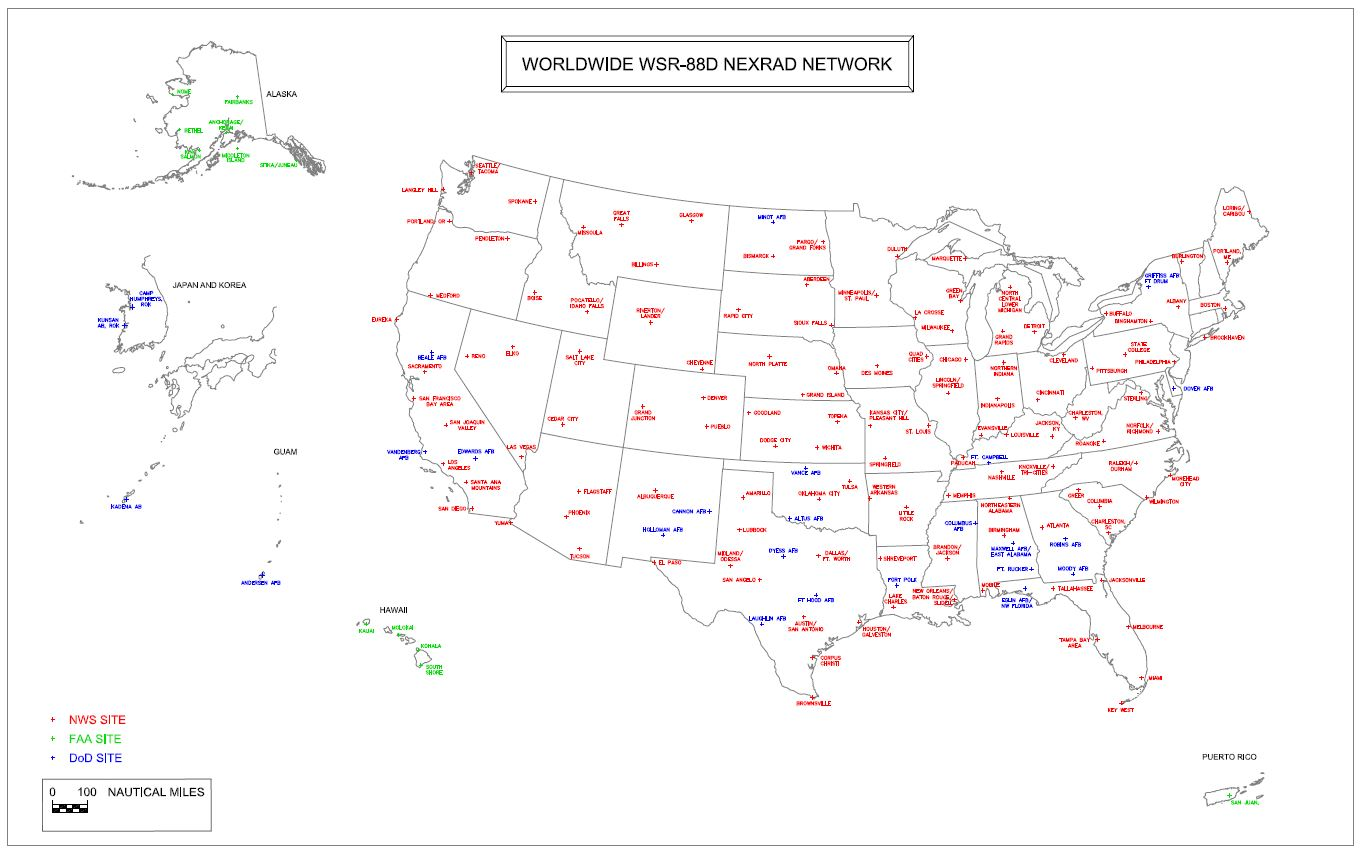
\includegraphics[width=\textwidth]{./thesis_code/plots/noaa_wsr88d_map.jpg}
	\caption{WSR-88D radar sites in the US and abroad. Image can be found at \url{https://www.roc.noaa.gov/WSR88D/Maps.aspx}}
	\label{fig:introduction_wsr88d-map}
\end{figure}

As such, it is urgent and appropriate to explore methods of analyzing the algorithms that have provided such insights in the natural image domain, and using techniques designed in the computer vision sub-field of transfer learning, attempt to extract information in weather radar image data.

\section{Research Objectives}
\label{sec:introduction_objectives}
% Rob: "This dissertation proposal aims to characterize wind turbine clutter with a focus on the dual-polarization signature of wind turbines in the presence of precipitation and ground clutter."
% First sentence is thesis statement after setting everything up

This dissertation proposal aims to develop an automated method for characterizing the spatial information available in weather radar scan data, utilizing information present in dual-polarimetric radar variables.
The long-term goal of this research proposal is to develop a set of automated methods to classify precipitation regimes and to illustrate the feasibility of deploying these models on voluminous weather radar datasets to extract insights and populate semantic tags to facilitate Data Discovery.
This proposal also aims to demonstrate that information available in natural image datasets and the models trained upon these datasets can transfer learning to the domain of weather radar data, allowing researchers to develop their own tools and locate specific atmospheric phenomena of interest by following the techniques presented herein.

Hand-labeling can and must be employed to generate an initial dataset for training the target task, image classification of precipitation regimes.
Once this is completed, techniques from the computer vision sub-field of Transfer Learning can be used to train models to learn functions to perform this classification.
The optimal models above can be determined via theoretical and empirical testing using readily available benchmarked datasets.
An iterative process can be then embarked upon to deploy the model on new data to perform classifications and increase dataset size.
Using a combination of automated classification and hand-labeling of the new generated data, a satisfactorily large dataset can be generated to train new models and finalize learning.

The key points to be addressed in this research are:
\begin{itemize}
	\item Hand-labeling weather radar data to produce a dataset for initially training models
	\item Determining optimal end-to-end deep learning architectures for learning and classifying similar images from benchmark datasets
	\item Using radar reflectivity image data from a research radar network to perform precipitation regime image classification
	\item Demonstrating the encoding of multiple radar variables into three-channel images to enhance classification ability
	\item Deployment of learned models on unseen data available in research radar network to automate data discovery and further enhance dataset, ultimately producing a hand- and machine-labeled dataset to supply to other researchers
	\item Employing the model on the national network of weather radars in the NEXRAD system, thus demonstrating effectiveness of the model at multiple spatial resolutions and radar frequencies
	\item Utilizing tools like CHORDS to perform semantic image classification in real-time
\end{itemize}

\section{Proposal Overview}
\label{sec:introduction_overview}
% Discuss what's in the following sections in the proposal

Chapter \ref{sec:background} presents a review of necessary and relevant literature for this research, with a focus on previously developed methods in weather radar image analysis, as well as transfer learning. 
Additionally, some background information on the calculation of various radar variables is presented, with specific focus on relevant radar moments in this work and how they are visualized both in real-time, and stored on disk.
Finally, the weather radar networks examined in this research are discussed.

Chapter \ref{sec:meteorology} discusses the meteorological phenomena that can be seen in weather radar data, and how they present in the images as functions of radar variables.
Precipitation regimes are examined, with some atmospheric precursors and products discussed to explore the relevance of these patterns and why they should be the foci of this classification work.
The spatial and temporal characteristics of the radar returns are discussed within the scope of how they are viewed in the radar data, so as to better understand the textures and patterns that the deep learning architectures will learn to classify.

Chapter \ref{sec:classifying} details the experiments performed to select and train the deep learning models.
Initially there is a treatment of relevant concepts and math used in machine learning, to develop the nomenclature and standards that follow.
Both shallow and deep networks are discussed in brief as necessary.
An experiment is performed to select a convolutional base and illustrate the utility of using large models in transfer learning tasks.
A set of experiments designed to illustrate the learning ability of the selected convolutional base and top model are detailed, utilizing a readily available benchmark dataset called MNIST-Fashion, chosen to mirror both natural images as well as weather radar images.
Next, the target task of weather radar images are classified according to their corresponding precipitation regimes, using hand-labeled data from a radar in the CASA DFW Urban Testbed of X-band weather radars.
Finally, relevant concerns are detailed regarding the proposed research of deploying models on data from the rest of the CASA DFW network, using multi-channel data with multiple radar variables to produce pseudo-images that encode greater amounts of information for training and testing, and deploying models on the S-band WSR-88D NEXRAD radars.

Chapter \ref{sec:bestmodel} describes the effect of using the model obtained in \ref{sec:classifying} to classify images from two months in 2018 to increase dataset size, as well as the effect of applying new layer technologies to the deep learning architecture.
A new optimal model is discovered, trained, and then deployed on unseen data from 2019, and a brief statistical and climatological examination is performed based on these classifications.

Chapter \ref{sec:realtime} discusses advances in real-time weather radar data, and details the research in implementing weather radar data as a core component of the Cloud-HOsted Real-Time data Services in the geosciences (CHORDS) portal.
This chapter details a survey of current methods in real-time weather radar data visualization, along with modern cyberinfrastructure concerns related to the storage and visualization of weather radar data.
The current CF/Radial standard is discussed, as well as the importance in using such standards to promote findability, accessibility, interoperability, and reusability (FAIR) principles in the domain of weather radar data.

Chapter \ref{sec:summary} summarizes the findings in this research project, and outlines a few potential new avenues that have been opened up as a result of this work.

The Appendix \ref{sec:appendix-a-tools} discusses certain practical considerations for deep learning research and their use in this work.


\chapter{Background}
\label{sec:background}

% Initially part of a rough draft of a paper I was writing. This section is mostly about automated weather radar image analysis
One area of computational research into the meteorological nature of weather radar scans is in the field of meteorological object tracking. 
The goal of this field is to identify “storm cells,” areas of localized convective activity, track their history in terms of evolution, merging, and splitting, and make short term forecasts about where they are going. 
The definition of the storm cells themselves is a matter of some debate, though some basic definitions exist from the perspective of remote sensing, such as that of \cite{lakshmanan2010objective}, who defines the cells as comprised of a 30 dbz horizontal reflectivity across a spatial area of 20 km$^2$. 
This area of research is not directly related to the object of this study, which is to correctly label scans as containing stratiform or convective activity, though it is related, and could be easily applied to this classification problem with minimal extra algorithmic overhead.

There are several approaches to this problem that have been explored in using algorithms to perform these objectives. 
Thunderstorm Identification, Tracking, Analysis, and Nowcasting (TITAN) \cite{dixon1993titan}, is an early algorithm designed to perform a similar task on NWS NEXRAD data. 
Another heuristic method, this system utilizes an empirically-determined horizontal reflectivity threshold, $T_z$, to locate spatially contiguous runs of high intensity returns within this single bin to designate as storm centroids. 
The Storm Cell Identification and Tracking (SCIT) algorithm \cite{johnson1998storm}, seeks to improve upon TITAN’s approach mainly by adding more reflectivity bins with which to organize storm decisions. 
The algorithm attempts to locate storm cell centroids in NWS NEXRAD radar data, and follow them in space and time. 
This method operates on a radial-by-radial basis, binning reflectivity values, and then checking for spatial proximity of the binned regions, assigning storm cell centroid status to those spatially proximate areas of high reflectivity. 
As \cite{lakshmanan2009efficient} points out, these two methods are limited by their requirement that spatially adjacent pixels must contain horizontal reflectivity values within certain thresholds to be considered by the algorithm as components for storm cell centroid candidates. 
That work describes a method that attempts to find storm cells via usage of the watershed transform, a technique pulled from the field of image processing, with a few tweaks to ensure that it performs well with weather radar imagery. 
Namely, they propose altering the “saliency” and “hysteresis” levels to allow the watershed to identify mature and growing storm cells while weeding out false positives. 
This approach negates the need for empirically-chosen global thresholds for bins, as it considers all possible thresholds when classifying the image. 
However, the method requires significant data preprocessing prior to its application, including filters to remove high frequency image content and quantization of values, which may remove useful local features from the image.

\section{Neural Networks}
\label{sec:background_neuralnetworks}
% This may be too much detail but I think it would be relevant to set up nomenclature and discuss neural network basics in this section
% I expect some of the people reading this will be unfamiliar with terminology, and it feels necessary for the sake of completeness.
% There are some papers worth citing that should be cited here, maybe an open source book?
% Neurons, Gradients, Forward Propagation, Backward Propagation, Linear Regression, Outputs (sigmoid and softmax)
% Cartoon of densely connected neurons in a small network
%
% My current plan is to start with a basic treatment of NNs in the Classifying chapter, with math there, to set the table for the reader in the sections that follow.
% This section should be more like a history lesson, bringing in some of the more major efforts. Discussing all kinds of examples of problems solved by machine learning, identifying gaps where this work hopes to fill.

\section{Image Classification with Machine Learning}
\label{sec:background_imageclassification}

% Discussion on Image classification in the broader field of image data machine learning, so that these terms can be used later in the document
Image Classification is a sub-field of a larger umbrella of image data machine learning that also includes image segmentation and semantic understanding. It is, however, the first step to achieving these latter two. Image Segmentation refers to...

% Discuss here some of the most well known papers and concepts around classifying image data. Things like Dropout, ReLU, Dense, BatchNormalization, Exploding and Vanishing Gradients,

\section{Transfer Learning}
\label{sec:background_transferlearning}

Transfer Learning is most often used to learn target tasks that differ from source tasks but reside in the same natural image domain. However, these architectures have been used to classify and segment image data
There have been a few efforts to apply deep learning algorithms in the area of climate science, applying models to weather data. 
For example, \cite{liu2016application} applied a deep learning architecture called AlexNet \cite{krizhevsky2012imagenet} to locate tropical cyclones, weather fronts, and atmospheric rivers, in colormapped continuous spatial variables, like precipitation, temperature, and other meteorological properties.
They briefly describe issues surrounding the usage machine learning models developed for natural image data in a non-natural-image data domain, and focus their analysis on a continental data scale.


\section{Dual-Polarized Doppler Weather Radar}
\label{sec:background_dualpol}
% This section is somewhat boilerplate in our group, but the basics of weather radar should be discussed here so that the instrument producing the data used in this research is understood. 
% Maybe a page or two, some images?

One of the key benefits \cite{doviak2000considerations} in dual-polarimetric Doppler weather radar over its predecessor, single-polarization, is that allows observing not only power return from a volume of scatterers, but also identifying parameters related to shape.
This is due to its usage of not only one antenna polarization in transmit and receive modes, but two orthogonally polarized antennas, which convey both power return in the horizontal as well as vertical.
For low elevation scans, as in those employed in plan-position indicator (PPI) scans, which are the focus of this research, these shape parameters can convey a great deal more information for the radar engineer to use in analysis.
This information is used directly by radar meteorologists to determine relevant atmospheric parameters with respect to various weather phenomena, as well as to inform several types of algorithms concerned with extracting additional information from these scans.
It is relevant to survey some of these techniques briefly here as many of the phenomena described tie directly into precipitation regime, and the methods utilized to extract key information as below directly inspires and influences the research presented in this work.
Some efforts of note along with brief descriptions:

\begin{itemize}
	\item Hydrometeor classification - determination of scatterer type in radar scans
	\begin{itemize}
		\item Using dual-polarizaton data to identify winter precipitation \cite{thompson2014dual}
		\begin{itemize}
			\item Using data from multiple radars and radar frequencies, this work uses scattering theory and T-matrix simulations to develop an algorithm based on fuzzy logic to classify scatterers in radar gates by their predominant hydrometeor type.
		\end{itemize}
		\item Semisupervised scheme for hydrometeor classification \cite{bechini2015semisupervised}
		\begin{itemize}
			\item Uses a fuzzy logic method as above, but adds a k-means clustering component to take advantage of localized spatial similarity of precipitation type to improve classification in range-height indicator (RHI) scans
		\end{itemize}
	\end{itemize}
	\item Nowcasting and short-term forecasting
	\begin{itemize} 
		\item LSTM model for precipitation nowcasting \cite{xingjian2015convolutional}
		\begin{itemize}
			\item Utilizes a memory-based neural network architecture called long short-term memory (LSTM) with a novel addition of convolutional input layers to utilize spatial and temporal information in short-term rainfall intensity prediction 
		\end{itemize}
		\item TITAN \cite{dixon1993titan}
		\begin{itemize}
			\item Early and well-known set of algorithms for identifying and tracking thunderstorms using NEXRAD WSR-88D data, using many image processing techniques with thresholded spatial and temporal information
		\end{itemize}
	\end{itemize}
	\item Quantitative precipitation estimation (QPE) - counting how much precipitation has already occurred 
	\begin{itemize}
		\item QPE in the CASA DFW Urban Testbed network \cite{chen2015quantitative}
		\begin{itemize}
			\item This paper computes the real-time rainfall rate in high spatio-temporal resolution by using information available from multiple radars scanning similar areas, on different time scales
		\end{itemize}
	\end{itemize}
\end{itemize}

This section intends to acquaint the reader with some of the major derived radar variables, with a focus on those that are used in this effort to classify stratiform and convective precipitation regimes both from one another and from cases that represent neither.
For a full treatment of weather radar theory, with specific focus on signal processing, consult \cite{bringi2001polarimetric} and \cite{doviak2006doppler}.


\subsection{Moments}
\label{ssec:background_moments}
% Moments refer to the different radar variables. 
% Talk about the big ones: reflectivity, differential reflectivity, copolar correlation, velocity, spectrum width, specific differential phase
% 

There are a few important radar variables, also called moments, that are necessary to detail here.
First is radar horizontal reflectivity factor $Z_h$, which is perhaps the most commonly used and well-known variable.
The formula to calculate this moment is given by \cite{bringi2001polarimetric}

\begin{equation}
Z_h (\mathrm{dBZ}) = 10\log_{10}\left( \frac{\lambda^4}{\pi^5 \left|K_w\right|^2}\int \sigma_h(D)N(D)dD \right)
\end{equation}

whereas vertical reflectivity factor $Z_v$ is given by

\begin{equation}
Z_v (\mathrm{dBZ})= 10\log_{10}\left( \frac{\lambda^4}{\pi^5 \left|K_w\right|^2}\int \sigma_v(D)N(D)dD \right)
\end{equation}

In the above equations, $\lambda$ is the radar wavelength in meters, $\left|K_w\right|^2$ is the dielectric factor for water (see below), $\sigma_h$ and $\sigma_v$ are the radar cross section (RCS) from horizontal and vertical polarization, respectively, $D$ is the equivalent particle diameter in mm, and $N(D)d(D)$ is the number of drops in a given spatial volume denoted of size $dD$.
The dielectric factor for water can be calculated by

\begin{equation}
\left|K_w\right|^2 = \left|\frac{\epsilon_r - 1}{\epsilon_r + 2}\right|^2
\end{equation}

where $\epsilon_r$ is the complex relative dielectric constant of water.

These equations map somewhat to the return power at each polarization, which translates roughly to a proportionality between reflectivity and rainfall rate.
This proportionality has been the subject of frequent empirical study, and can be calculated when there is an overlap in radar coverage and ground instrument (like rain gauge) positions.
The relationship between the two is typically modeled as 

\begin{equation}
R (mm/hr) = \alpha Z^\beta
\end{equation}

where $\alpha$ and $\beta$ are constants that can be solved empirically.
Rain rate can be calculated as a function of various radar variables as inputs to algorithms of various complexity, and is itself a radar variable in its own right, often available to researchers for study alongside the others.

Scatterers like raindrops are typically oriented with respect to the ground according to a probability distribution, which is a function of drop size, air resistance, and wind.
Raindrops are not perfectly spherical at larger sizes, however, and as such, exhibit different levels of power returns in the vertical and horizontal polarizations.
As such, it is often interesting to compare the reflectivities in these polarizations, and in conjuction with horizontal reflectivity, some hydrometeor classification between large raindrops (more oblate -> higher difference between $Z_h$ and $Z_v$) and hail (high $Z_h$, similar $Z_h$ and $Z_v$) can occur.
This is another radar variable, called differential reflectivity, given by

\begin{equation}
Z_{dr} (dB) = Z_h - Z_v
\end{equation}

Since $Z_{dr}$ relies information on axis ratio, scatterer canting angle, and scatterer size, it can be used to identify scatterers which may be present under only a stratiform or convective precipitation regime.

Another useful radar variable is \textit{specific differential phase}, which is the bulk phase shift due to scatterers in a range volume, and is formally defined as

\begin{equation}
K_{dp} (\deg / \mathrm{km})= \frac{180}{\pi}\lambda \mathrm{Re} \left[\int \left[f_h(D)-f_v(D)\right]N(D)dD\right]
\end{equation}

where $f_h$ and $f_v$ are complex forward scattering amplitudes at eahc polarization.
Because radar cannot directly measure $K_{dp}$, we can use the accumulated differential phase shift $\Phi_{dp}$along each radial and take its range derivative to provide the estimate

\begin{equation}
\hat{K_{dp}} = \frac{\Phi_{dp}(r_2)-\Phi_{dp}(r_1)}{2(r_2-r_1)}
\end{equation}

This parameter can be difficult to estimate and there are many methods, ranging from the simple estimate above to adaptive parametric aprroximations \cite{wang2009algorithm}.

The fourth major variable we can compute is called variously correlation coefficient, copolar correlation coefficient, and cross polar correlation coefficient, and seeks to provide an estimate of how similar scatterers within a range volume are to one another.
It can defined as

\begin{equation}
\rho_{hv} (0) (\mathrm{unitless}) = \frac{\left\langle S_{vv} S_{hh}^* \right\rangle}{\left\langle S^2_{hh}\right\rangle^{1/2} \left\langle S^2_{vv}\right\rangle^{1/2}}
\end{equation}

where $S_{hh}$ and $S_{vv}$ are the horizontal and vertical components of the backscattering matrix, $*$ is the complex conjugate operator, and $\left\langle\right\rangle$ are ensemble averages.

Velocity and corresponding spectrum width variables can be calculated via Fourier analysis of the complex IQ returns, and can be useful in informing meteorological analysis, but will not be covered here as they're not used in this research work.
Additionally, there are many potential radar variables.
For more information, refer to \cite{bringi2001polarimetric} or the CF/Radial specification \footnote{\url{https://ral.ucar.edu/projects/titan/docs/radial_formats/CfRadialDoc.pdf}}.

Examples of the four radar variables can be seen in Figure \ref{fig:background_radarvar_examples}.
The plots were produced using python, matplotlib, and Py-ART, with colormaps from the colorcet library and Py-ART.

\begin{figure}[h]
	\centering
	\includegraphics[width=\textwidth]{./thesis_code/plots/20160511_radar_variable_examples.png}
	\caption{Examples of radar variables, left to right, top to bottom: $Z_h$, $\rho_{hv}$, $Z_{dr}$, and $K_{dp}$. Case from 2016-05-11, XMDL Radar, CASA DFW network. This particular scan is from the stratiform precipitation regime, as evidenced by relatively low $Z_h$, high $\rho_{hv}$, and middling $Z_{dr}$.}
	\label{fig:background_radarvar_examples}
\end{figure}

\subsection{Colormapping}
\label{ssec:background_colormap}

The term “colormapping” refers to the process of converting numerical data, usually held in arrays of more than one dimension, and mapping the values to a set of colors for representation on an image. 
This is most often done in the sciences as a way for humans to be able to more readily understand trends in the data, or identify features of interest. 

In the domain of weather radar data, the most obvious way to represent the variables associated with returns from precipitation is by producing a plot where the image is centered on a radar (or radars) of interest, and mapping the values in specific moments to colors via a colormap. 
The choice of colormap is important, and the optimal choice may not be obvious.

Typically, radar reflectivity factor ${Z_h}$ is represented via a “rainbow” style colormap, with high values of dBZ in the ‘warm’ region of the color space, such as oranges, reds, pinks, and yellow, while lower values correspond to ‘cool’ colors, i.e, greens, blues, and purples. 
This is intended to assist the viewer in quickly identifying regions of high returns that could correspond to intense rain or hail, while visually separating these from areas of medium returns or lower return values that would indicate more sedate forms of precipitation, and thus, less dangerous. 
The intuition behind the initial studies that motivated this work were based on these simple assumptions: specifically, that if humans could use the colormapped data in the images to make inferences regarding the content of said images, then perhaps this process could be automated using techniques developed by the computer vision community.
As such, it becomes important to assess the choice of colormaps themselves. 
Even within the weather radar community, there is disagreement as to which specific colormap should be used when displaying data from any variable. 
Continuing with the examination of ${Z_h}$, there are a few major colormaps that are used by different groups that are worth discussing here, such as NWS Reflectivity and CSU-CHILL. 
Additionally, when prototyping code or doing basic exploration of the data, many groups have resorted to using the ‘jet’ colormap to display the data.
See Figure \ref{fig:background_colormap_examples} for examples of some of the above colormaps, along with perceptually uniform colormaps provided in the colorcet library.

\begin{figure}[h]
	\centering
	\includegraphics[width=\textwidth]{./thesis_code/plots/20160511_colormap_examples.png}
	\caption{Examples of colormaps. Case from 2016-05-11, XMDL Radar, CASA DFW network. Variable plotted is Corrected Reflectivity $Z_h$. Notice how in the perceptually uniform colormaps 'rainbow' and 'bmy' that it is easier to quickly detect textures within the precipitation regions of the image. The NWS colormap draws the eye to the red regions, which correspond to higher reflectivities, and 'jet' fails to do either.}
	\label{fig:background_colormap_examples}
\end{figure}

While it is clear that it is disadvantageous to use the colormap, ‘jet’ has its advantages, but many visualization guides advise moving away from its widespread usage in science data. 
This discussion is more relevant below in section \ref{sec:CHORDS_colormap}, where selection of colormaps is aimed at allowing human eyes and human brains the highest advantages possible in the display of nominal weather radar image data, but there are questions that need answering here, too, with respect to how a machine can best learn from image data. 
Such questions include: Does a convolutional neural network make more robust classifications if different regimes of colormaps are employed on the same data? 
As a colormap can be thought of as a quantization of data, do the bin intervals matter with respect to classification? 
Do the intervals need to be uniformly spaced, as is often done for human inference? 
Does the quantization help, or is it better to focus on the raw data? 
Experiments will follow to test these questions and outline the results.

It is pertinent here however to discuss the types of colormaps that are generally used to display image data in science. 
Specifically there are a few major categories, which I will refer to as ‘rainbow,’ ‘diverging,’ and ‘linear.’
Rainbow colormaps tend to be employed where data in different intervals may correspond to different phenomena or regimes, and can be used to display categorical or “categorical-adjacent” datasets. 
In radar data, rainbow colormaps are used to represent horizontal and vertical reflectivity factors. 
Diverging colormaps are used to demarcate a point in the data, and highlight values increasing or decreasing from that point. 
A common example in weather radar data is velocity of scatterers, where warmer colors may indicate increasing radial velocity away from the radar, while cooler colors would correspond to increasing radial velocity towards the radar, with 0 meters per second being the point of demarcation. 
This colormap is also appropriate to log differential reflectivity, where 0 dB describes a volume where scatterers are equivalent in shape in both horizontal and vertical directions. Finally, linear colormaps tend to be used to describe intensity data. 
This would apply to specific differential phase, cross polar correlation coefficient, and normalized coherent power data.

\section{Weather Radar Networks}
\label{sec:background_networks}

Weather radar, like any instrument, is most valuable when considering the context of observed phenomena in the greater geospatial region. 
As such networks of weather radars are maintained and operated globally. 
This dissertation focuses on two such networks: namely, the Collaborative Adaptive Sensing in the Atmosphere (CASA) Dallas-Fort Worth network, and the WSR-88D NEXRAD network. 
There are further examples that may warrant attention in future work, such as systems operated by the Department of Energy in the United States, though it is expected that the techniques and results achieved here would be applicable to other systems as well.

\subsection{CASA DFW}
\label{ssec:background_casadfw}

The CASA DFW radar network is a network of 9 X-band weather radars in the greater Dallas-Fort Worth (DFW) urban metroplex, as demonstrated in Figure \ref{fig:background_casamap}. 
It represents efforts by the U.S. National Science Foundation Engineering Center (NSF-ERC) for Collaborative Adaptive Sensing of the Atmosphere (CASA) made over the past 15 years to design a system to address problems regarding the curvature of the Earth and gaps in NEXRAD radar coverage due to ground clutter \cite{chen2015quantitative}. 
The Dallas-Fort Worth urban metroplex is a large-scale, high population, complex cityscape, and prone to damage and loss of life with respect to natural disasters like flash floods, tornadoes, and hail. 
The network utilizes X-band radars operating in concert to assist nowcasting and disaster preparedness by providing relevant safety officers and stakeholders with composite radar data in high-resolution in both time and space. 
X-band systems were chosen in part due to their high-resolution spatial querying, and their lower footprint and operation cost as compared to S-band radar systems.

\begin{figure}[h]
	\centering
	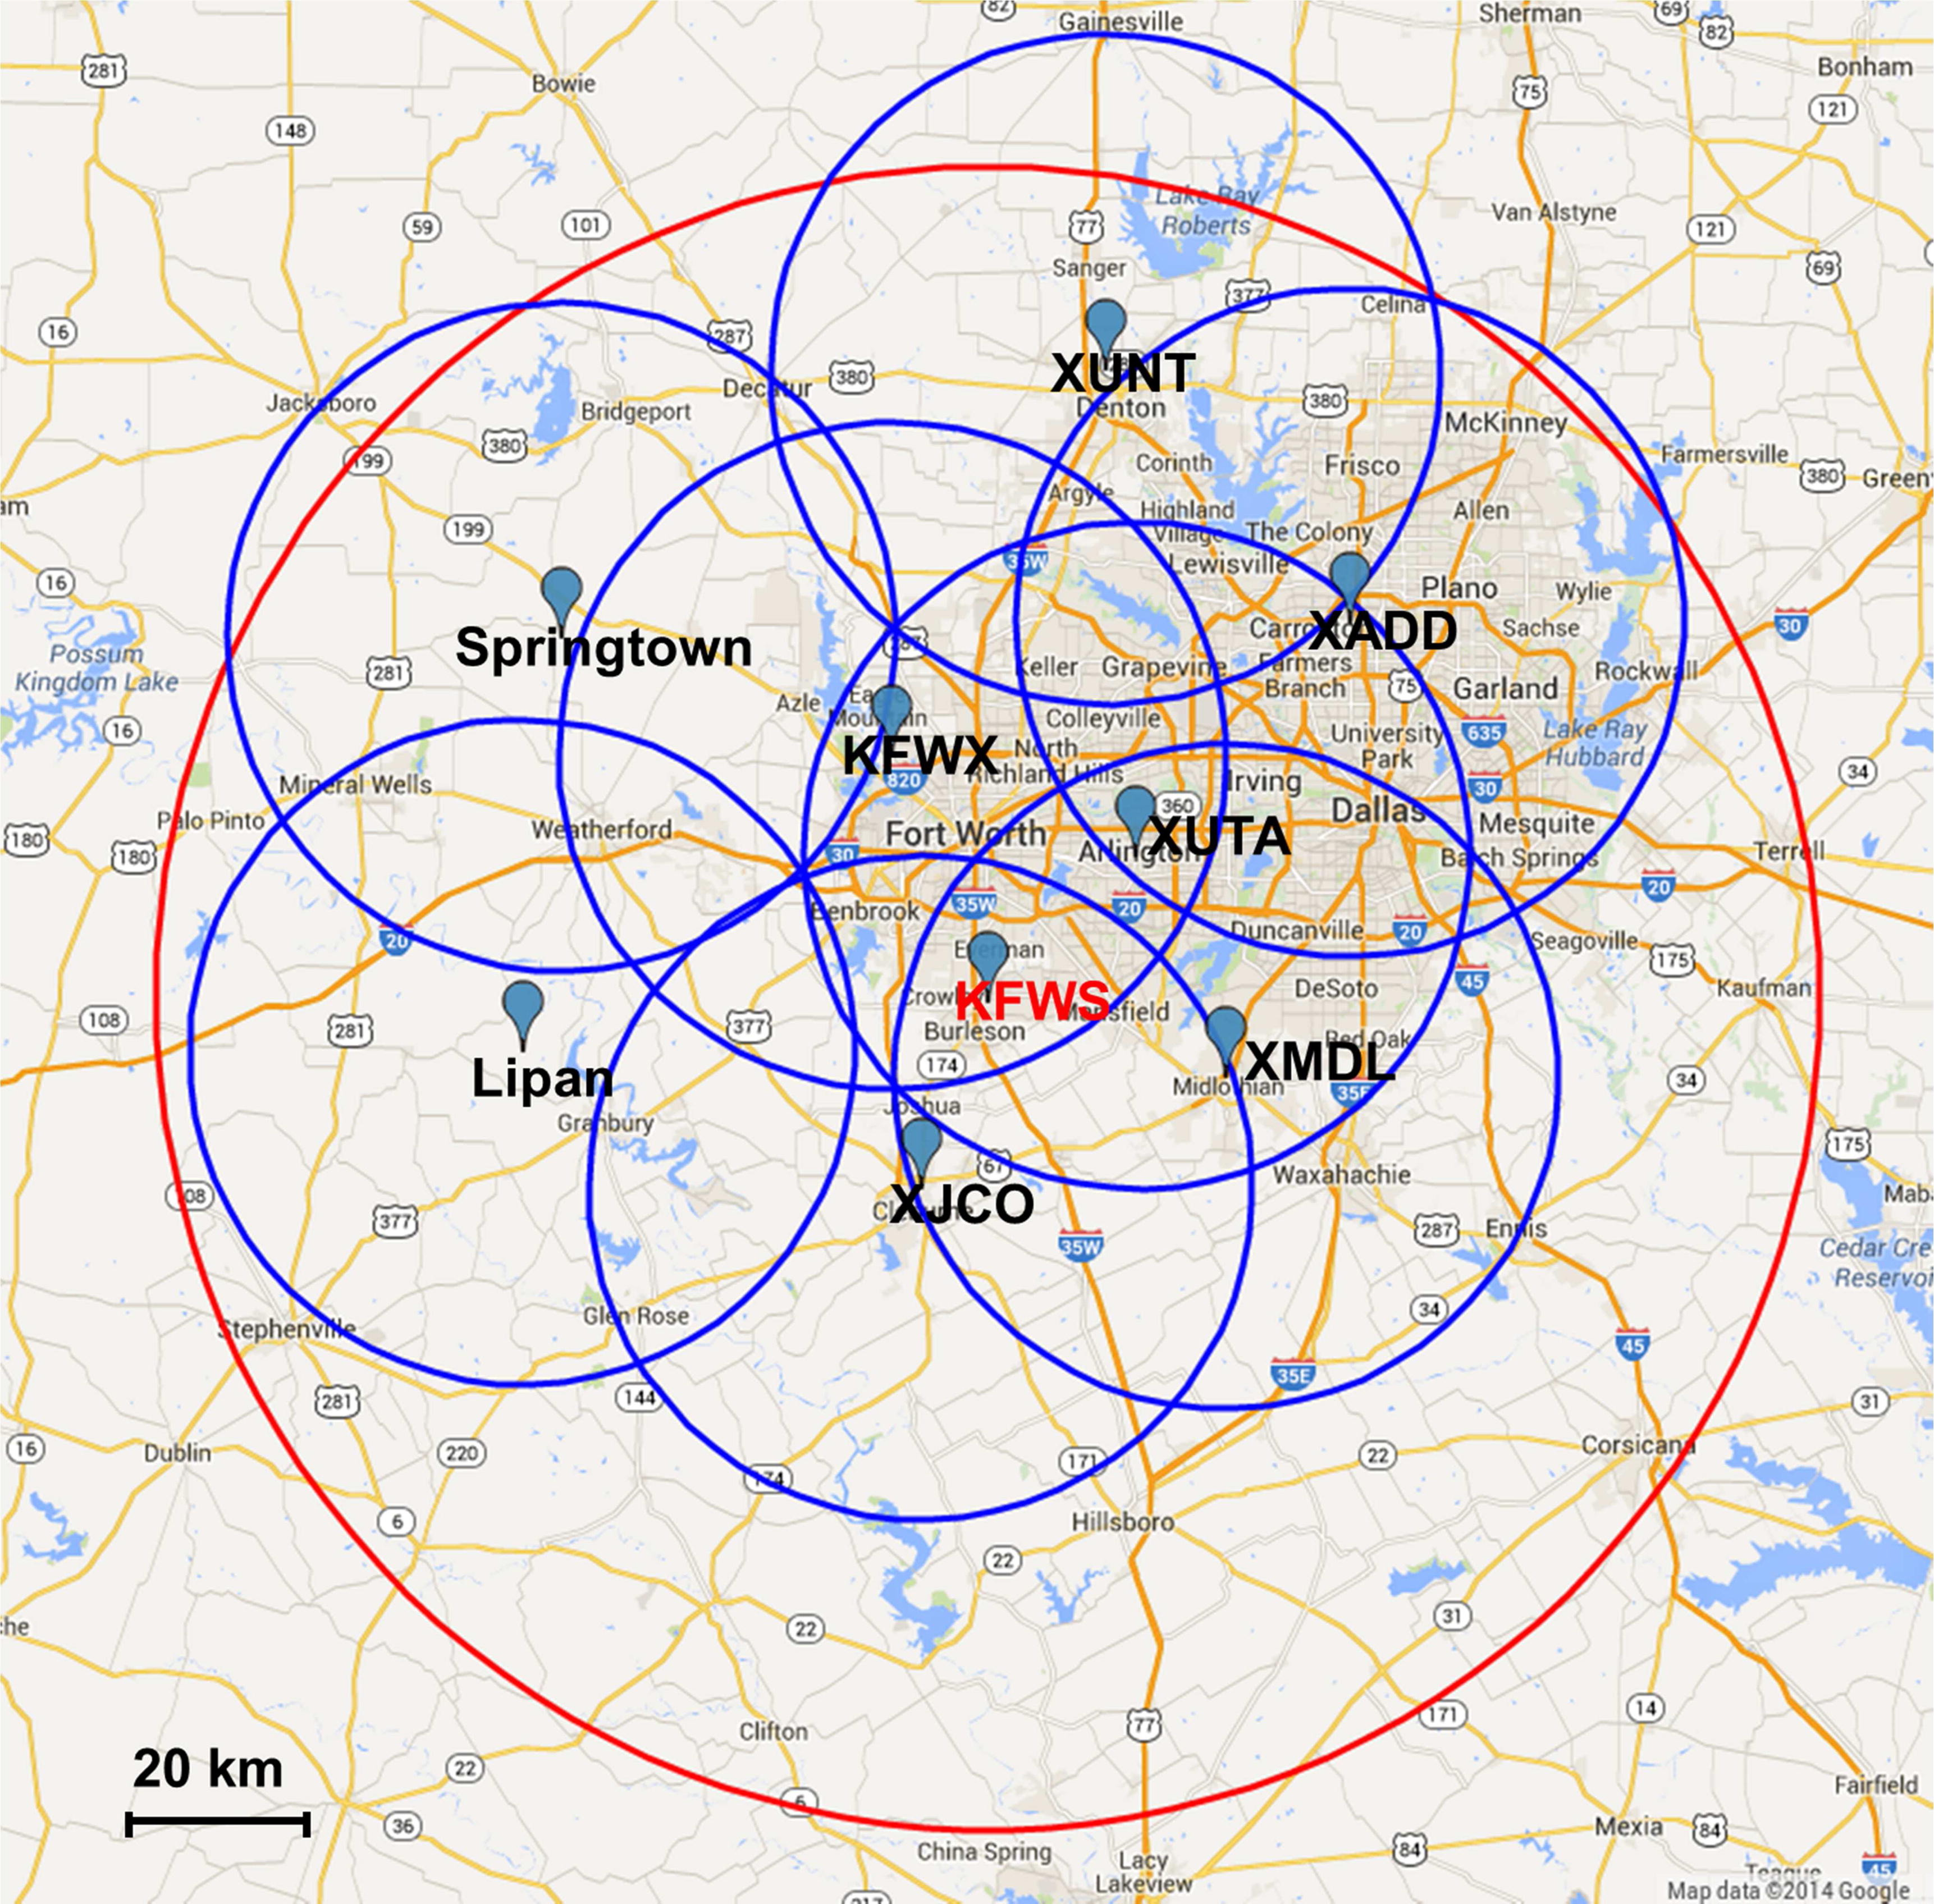
\includegraphics[width=\textwidth]{./thesis_code/plots/casa_dfw_map.jpg}
	\caption{The CASA DFW Urban Testbed network of dual polarimetric X-band Doppler weather radars \cite{chen2015quantitative}, plotted on Google Maps.}
	\label{fig:background_casamap}
\end{figure}

Many of the features and products provided by the CASA DFW system are irrelevant in the present work, including the three-dimensional wind fields and high-resolution rain rate products.
Instead, this research focuses on classifying images produced from single weather radars, and as such can use dual-polarimetric radar variables from each of the radars in the network individually.
Data from each radar in the network are analyzed by signal processing servers at each radar, and the radar variables are stored at the DFW Radar Operations Center (DROC) in two ways: first, all moment data from each completed PPI scan is stored in NetCDF-format files on DROC servers; and second, Portable Network Graphics (PNG) files are generated at each of three elevation scan angles, for each of four radar moments, including horizontal reflectivity, copolar correlation coefficient, differential reflectivity, and radial velocity.

\subsection{NEXRAD}
\label{ssec:background_nexrad}

NEXRAD is a network of WSR-88D S-band radars that are intended to provide weather radar data throughout the United States with minimal gaps in coverage. 
The above concerns regarding Earth curvature, ground clutter, and coverage gaps notwithstanding, the network represented a massive undertaking by the National Weather Service, and serves to this day as a major data provider in the geosciences. 
Recently, the data was moved to be stored in Amazon Web Services cloud storage, further increasing ease of access for recent and historical weather data. 
The data produced from this network is used in weather prediction, as comparison with other sensors, and as inputs to high resolution models for short-, medium-, and long-term forecasting.

When testing these models, atmospheric data scientists are presented with many challenges, including identifying phenomena of interest in the prohibitively voluminous datasets. 
As such, it is of critical importance to develop automated methods for discovering insights and phenomena that are present in the available data, as a way to build datasets and improve forecast model fidelity.

\chapter{Radar and Meteorology}
\label{sec:meteorology}

For most of the 20th and early 21st century, weather radar has provided the highest resolution and most complete snapshot of meteorological phenomena. 
Some recent work has illuminated methods for developing even higher resolution weather data solutions by analyzing cellular communications data, but for most in the academic realm of geosciences, weather radar remains the most trusted and most available instrument for observing the atmosphere and meteorological phenomena.

Since this work focuses on identifying and classifying meteorological phenomena in weather radar scans, some discussion is warranted on what features can be observed in this data format, how humans analyze weather radar data, and solidifying the terminology used throughout this document.

\section{Precipitation Regimes}
\label{sec:meteorology_precip}

Essentially, we examine two major precipitation regimes: stratiform, and convection.
Examples drawn from the hand-labeled dataset of scans observed by the XMDL radar in the CASA DFW network are shown in Figure \ref{fig:meteorology_examples}.

\begin{figure}[h]
	\centering
	\begin{subfigure}[b]{0.45\textwidth}
		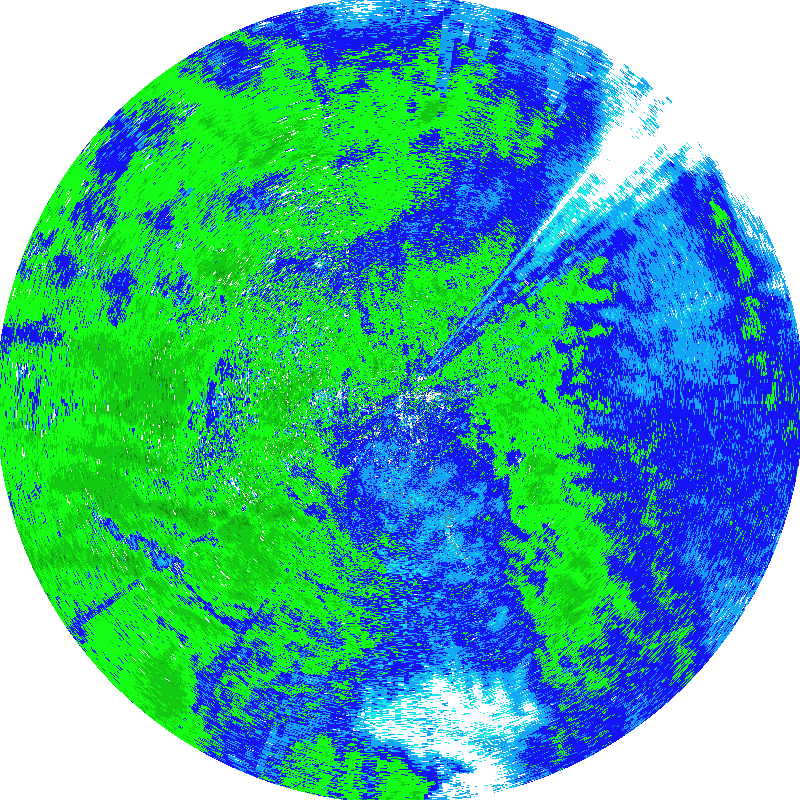
\includegraphics[width=\textwidth]{./thesis_code/plots/midlothian-tx-20170807-052557-ref-STRATIFORM.png}
		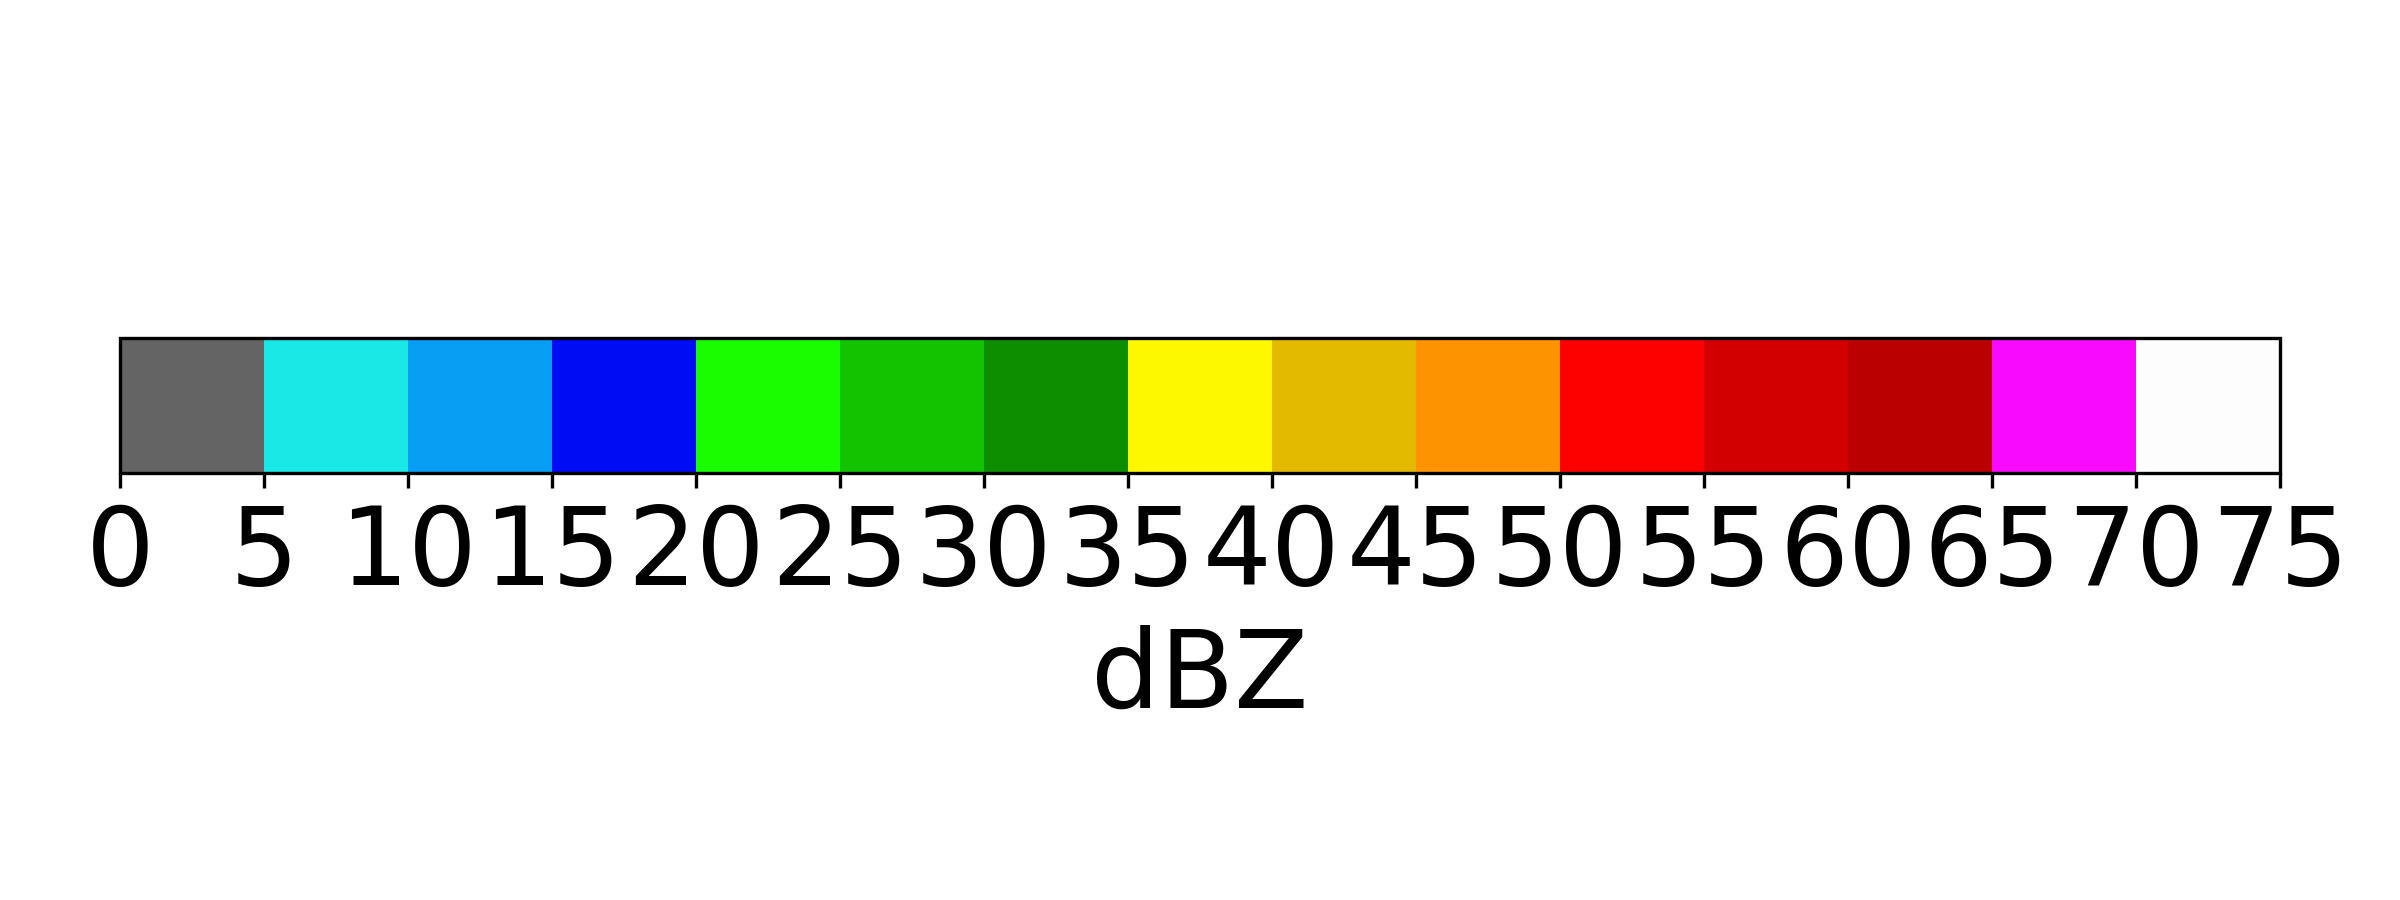
\includegraphics[width=\textwidth]{./thesis_code/plots/dfw_colormap.png}
		\caption{Stratiform - 2017-08-07 06:30:34 UTC}
		\label{fig:meteorology_stratiformexample}
	\end{subfigure}
	\begin{subfigure}[b]{0.45\textwidth}
		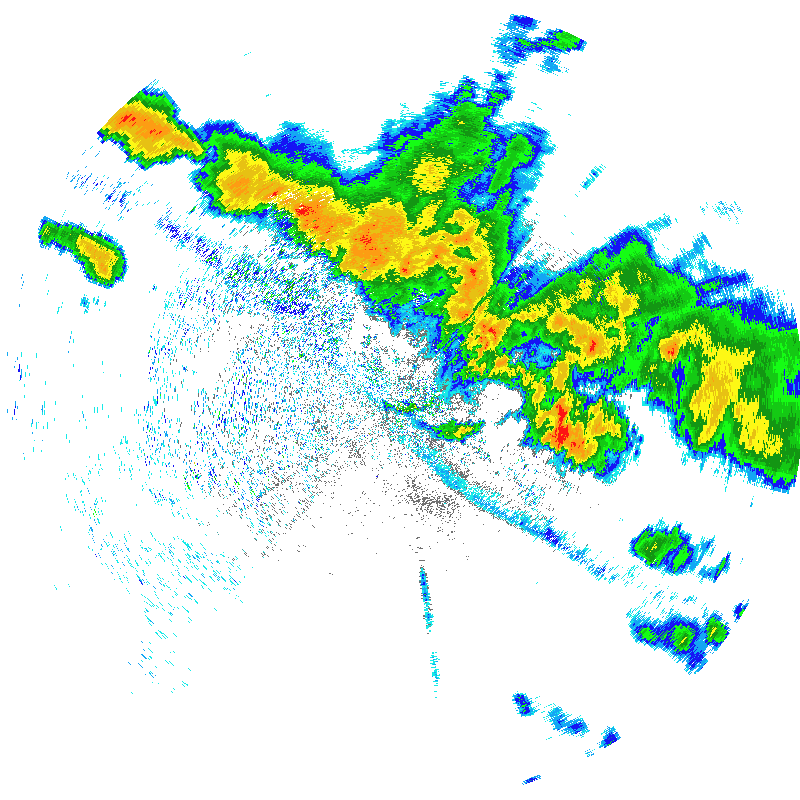
\includegraphics[width=\textwidth]{./thesis_code/plots/midlothian-tx-20170624-063034-ref-CONVECTION.png}
		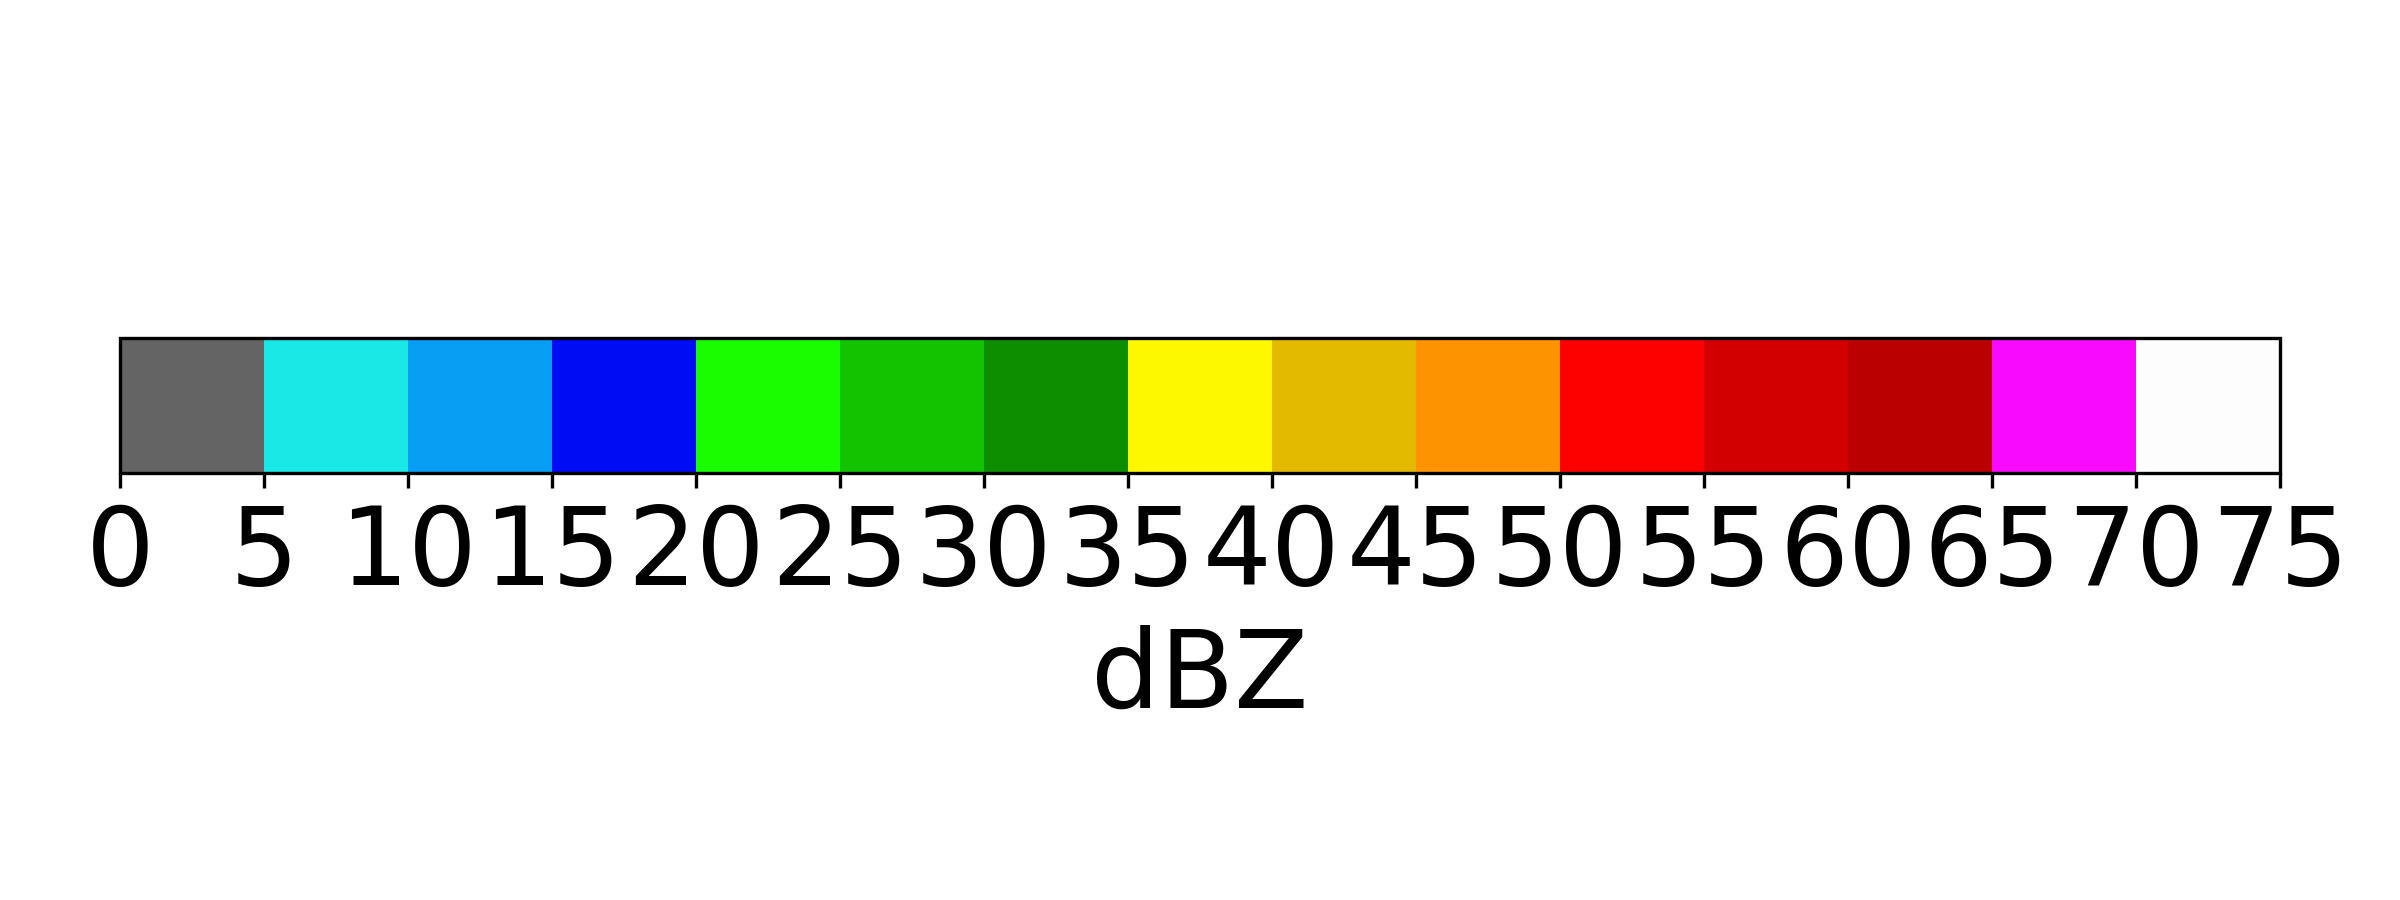
\includegraphics[width=\textwidth]{./thesis_code/plots/dfw_colormap.png}
		\caption{Convection - 2017-08-07 05:25:57 UTC}
		\label{fig:meteorology_convectionexample}
	\end{subfigure}
	\caption{Examples of radar reflectivity $Z_h$ from the two major precipitation regimes, observed by the XMDL radar in the CASA DFW network}
	\label{fig:meteorology_examples}
\end{figure}

Unfortunately, there is no hard and fast definition for what either of these particular regimes are.
It would be satisfying to be able to point out a few membership functions for radar parameters, as well as some specific atmospheric generating processes, as a way to conveniently put every precipitation radar scan into one of the two bins.
In fact, the former must be done to produce a training dataset, but it is worth noting here that this is something of a fiction.

\section{Radar Observations of Meteorological Echoes}
\label{sec:meteorology_echoes}

% combine the two sections above? I think so. Or just delete section{weather phenomena}

The highly cited ($>$ 650) "Stratiform Precipitation in Regions of Convection: A Meteorological Paradox?"\cite{houze1997stratiform} published in 1997 in the Bulletin of the American Meteorological Society attempts to provide a definition for stratiform precipitation, that we will use as a basis for the analysis in this work.
To wit: 
"Stratiform precipitation is fairly homogeneous in the horizontal, giving it a layered structure in vertical cross sections of radar reflectivity. In particular, it often exhibits a pronounced layer of high reflectivity called the "bright band," marking the layer in which the downward settling ice particles are melting."
Additionally, the authors contrast this with convection, which they aver can be detected on radar scans via pronounced cells of high reflectivity, corresponding to \textit{storm cells}, another term with loose definition.
The paper points out that storm cells typically feature spatially localized intense returns, that when viewed vertically in a range-height indicator (RHI) scan, appear to have a much taller core, and less pronounced bright band, than do the more spatially uniform stratiform precipitation scans.

It is with this knowledge that we turn our attention to plan-position indicator (PPI) scans, where elevation is fixed, and the radar scans in azimuth. 
In these scans, especially at lower elevation angles, there is far less of a chance to see a bright band, or melting layer.
However, stratiform regimes tend to produce more spatially uniform reflectivity returns over a large coverage area, whereas convection regimes produce cells of intense precipitation or hail, and correspondingly intense reflectivity returns, over smaller areas.
One final possibility is that convection can occur within a largely stratiform region, so there is overlap, from the perspective of the bulk image classification.

Other research efforts have attempted to use horizontal reflectivity data from PPI scans in classifying the two regimes. 
Along with pointing out the meteorological interest in discerning data of this type, \cite{biggerstaff2000improved} presents an algorithm that itself improved upon a prior work \cite{steiner1995climatological} via the Tropical Rainfall Measuring Mission (TRMM) to partition stratiform and convective regions within individual volumetric scans. 
This latter work points out the difficulty in using the melting layer identification as a method for performing stratiform vs convection classification: namely,

\begin{enumerate}
	\item Vertical resolution of weather radar scans (in PPI mode) are inadequate to resolve the melting layer except near the radar, limiting the sampling area
	\item The melting layer is not always well-developed even in stratiform regimes, especially in early-stage or late-stage stratiform, or in scans where both types of precipitation are present
\end{enumerate}

The authors describe a condition for the determination of stratiform precipitation in terms of a vertical updraft wind speed $w$:

\begin{equation}
|w| << |V_t|
\end{equation}

where $V_t$ is the snow particle terminal velocity, for particles above the melting layer.
In convection, this updraft speed is higher with respect to the fall speed, leading to particles growing in a different manner, and generating much larger rain drops or hail by the time they reach the ground.

By inference, and as stated above, in stratiform rain cases, precipitation is more spatially uniform than in convection, and this fact is utilized by \cite{steiner1995climatological} to perform classifications using the horizontal structure of the precipitation field. 
They convert the polar weather radar volume scan to a three-dimensional Cartesian grid, then look for peaks in the rain rate, which is directly proportional to reflectivity.
By defining and combining criteria regarding the intensity of reflectivity values, the number of peaks outside a convective center, and statistics from the surrounding area of the convective center, they make classifications regarding precipitation types in scans for specific regions.

This method utilizes information about the atmospheric processes and how they present in the highest resolution data available to perform classifications. 
However, its reliance on well-calibrated rain rate returns, available only via empirical determination and variable not only between locations but also in time limits the utility of this method in producing high fidelity classifications for other radars.
Furthermore, its statistics regarding reflectivity field values may not correspond to optimal discriminating functions for the two regimes, a drawback in any method that relies on heuristics, design choices, and other hyperparameters to determine a suitable function.

As we will discuss in Chapter \ref{sec:classifying}, one advantage in utilizing machine learning algorithms as tools for functional approximation is that many of the above design choices, parameters, and nonlinear mappings can be learned by models well-suited to the task.
This is not a new concept, of course, and early attempts using neural networks have been tried by other groups for performing these classifications. 
In one example \cite{anagnostou2004convective}, a shallow, three layer neural network consisting of two hidden layers of 8 neurons each was developed and trained on a set of features chosen by the authors.
The features included storm height, reflectivity values at specific elevations above ground level, height of maximum reflectivity level, vertical gradient of reflectivity, and horizontal reflectivity standard deviation.
This last feature ties in directly to the discussion above, whereby variable spatial returns may be less likely to be considered stratiform precipitation regimes.

As above, the classification was performed on WSR-88 reflectivity data, but this study utilized radars throughout the southeastern United States, as compared to only one platform in the previous regime.
Compared to the aforementioned methods, the false alarm rate in classifying stratiform was comparable, but was far superior to classifying convective precipitation than the others.
And false alarm rate (FAR) is perhaps the most important metric when considering data discovery, where the results of any algorithm are expected to represent the class that the algorithm labels them.
This study also demonstrated the value in utilizing neural networks as a functional approximation technique, and their strength in finding feature spaces where decisions can be more readily made.

The neural network in \cite{anagnostou2004convective} was impressive but only could learn a linear function, given its structure.
Additionally, the features in the network were drawn from a low-resolution 2 km x 2 km grid, which may have smoothed over local variability of interest.
Finally, the feature engineering provided valuable predictors, yet overlooked the raw two-dimensional textures inherent in radar reflectivity data, that form a large component of how humans perform precipitation regime classification.

Other methods have been shown to perform this classification and include instruments other than weather radar, such as disdrometers \cite{caracciolo2006analysis} and satellites \cite{feidas2012classifying}.
These systems are vaulable tools and can provide information to those with access to the data, but require either specialized instruments to implement, or correspond to smaleler-than-desireable coverage areas than weather radar, and as such will be ignored in this analysis.

\chapter{Classifying Meteorological Observations in Radar Image Data}
\label{sec:classifying}

%Might need to have more information on general data handling. 
%One idea: Do some in-class similarity statistics on various classes in meteorology data as well as some toy dataset. 
%Might need to have entire section on toy dataset even.

A question of particular interest is that since most available convolutional bases are trained on photographic images, can the knowledge from the structures, textures, and features they extract be applied to data outside the natural image domain?
These models are trained for 3 input channels, which are usually red (R), green (G), and blue (B), to form the 3-tuple denoted RGB.
In the \textit{reflectivity alone} case, there is a single channel of image data, which is simply the $Z_h$ intensity value.
There is usually, however, color information that is applied to this data via a colormap, which both quantizes the data and assigns color to this data bins. 
This is usually intended as a method to enable ease of visualization for humans, both in real-time analysis as well as when examining prior data.
A common practice to facilitate the human-data-discovery pipeline is to store generated images as \textsc{png} files, or some other image specification.

As such, this method sets up a convenience in data processing, if it can be incorporated into a machine learning pipeline as a direct input, thus saving costly steps involving file I/O, reading specific variables data, and processing into a suitable format. 

This leaves a few specific questions for this work:

\begin{itemize}
	\item Can a deep learning (DL) model learn from and properly classify single channel data?
	\item Can it do so from a colormapped version of the data?
	\item Is there a specific colormapping technique that would yield a more suitable or even optimal mapping ot use as input to a DL model?
\end{itemize}

We designed and present a few experiments, designed to answer these questions.
The first question is one that is key in this dissertation.
Put another way, can low- and mid-level image features be used in weather radar image data to identify and classify precipitation regimes?
This question will be answered over the course of this manuscript.
However, the following two questions need to be addressed as part of this, and will be examined first.

One way that Deep Learning architectures can be thought of working is via extracting image features and analyzing the spatial and pixel-based content, then using these features to discriminate between classes.
RGB tuples are usually the input, which gives 3 independent channels of data for the DL models to analyze.
As such, it seems unlikely that the specific colors used would matter, so long as the space was appropriately trained and modeled, and test images remain consistent with training images.

In order to test this hypothesis, we examine a few colormapped versions of the input MNIST Fashion dataset, which contains $N=60000$ training samples encompassing 10 classes relating to categories of clothing.
The usage of this dataset is to provide a point of comparison for the model accuracy and loss curves generated in this research with benchmark values produced by others in the field.
We will illustrate the design choices regarding constructing and training the end-to-end deep learning model architecture using this dataset prior to implementing it on the desired target dataset of precipitation regimes.
Specifically, we perform the following experiments to answer the following questions:

\begin{itemize}
	\item With many available choices of carefully trained convolutional base models available in the field, which to choose?
		\item Experiment: Compare classification curves of two such models, VGG16 and MobileNetV2, using MNIST-Fashion dataset
	\item Does colormap matter?
		\item Since many available processed weather radar scans involve colormapped data designed for human evaluation, it is important to discover if colormapping intensity values has a deleterious effect on model learning
		\item Experiment: Encode the MNIST-Fashion images in three colormaps, and compare validation accuracy of chosen model on each dataset, which are detailed here:
		\begin{enumerate}
			\item Black \& White: Raw data duplicated in three channels
			\item Viridis: Perceptually uniform, to faithfully match colormap design to data characteristics
			\item NWS Reflectivity: Mapping data to rainbow colormap preferred by the National Weather Service to represent horizontal reflectivity data
		\end{enumerate}
	\item How much can we learn?
		\item Train model on each dataset until maximum learning is achieved in top classifier, then fine tune model to maximize learning on target dataset
\end{itemize}

This chapter first introduces image classification and develops a brief but necessary background in techniques and advances that lead to solving problems of the kind in this work.
There are several conventions regarding nomenclature and formal description of this sets of problems and solutions.
As such, it is critical to establish a convention to be used throughout this document.
Additionally, the open source movement in the research fields has led to an increase in open access publications.
Following along in this spirit, this document will attempt to follow conventions set by respected, oft-cited, open access materials, such as \cite{goodfellow2016}.

\section{Image Classification}
\label{sec:classifying_image}

In order to understand image classification, transfer learning, and the application of these to weather radar images, we must first examine the basics of machine learning, and carry this examination through deep neural networks (DNNs), how these models are developed, and how features can be extracted from images and used to generate predictions, classifications, and ultimately, to generalize to unseen data. 
It is expected that the readers will have had some prior experience in studying machine learning techniques, and as such, the examination here will not be exhaustive. 

It is perhaps important here to specify that image classification is one sub-type of classification problem that is discussed in image-based deep learning literature.
Image classification is to make an inference about the class to which an image belongs in its entirety. 
Contrary to this is object detection, which seeks to find localized objects in a given image.
In object detection, there can be multiple instances of a given object in any image, and it is expected that there are many types of objects that may or may not be present in any image given to the system.


\subsection{Machine Learning Concepts}
\label{ssec:classifying_concepts}

% Training/Testing, Classification/Regression, Supervised
We can define machine learning as a methodology for allowing a program "to learn from an experince $E$ with respect to some class of tasks $T$ and performance measure $P$, if its performance at tasks in $T$, as measured by $P$, improves with experience $E$," as described in an early book \cite{mitchell1997} on the topic. 
This verbalizes and formalizes the experiment space in which machine learning algorithms live.
In this terminology, the task $T$ is what we seek to achieve; in this work, this is always a classification of input data into categories, such as classifying weather radar. 
The experience $E$ is the data that the model learns from, and consists of two types of datasets, referred to as \textit{training} and \textit{validation} data. 
In \textit{supervised learning} problems, the umbrella under which the problems in this work exist, the training and validation datasets have labels corresponding to the correct classification.
These labels are used to teach the model how to classify the data samples presented during the training phase.
Additionally, the validation set is a group of data samples representing a stratified random sample of all samples available in training, and is used to evaluate the model during training to provide information to both the model itself and the researcher.
The performance measure, $P$, is how the predictions of the model are evaluated, which usually takes the form of an \textit{accuracy}, which is computed as the fraction of correctly predicted values to the total number of values.
This is evaluated on a held-out \textit{test} set of data, which is a simulation of unseen data, and is useful as a measure of the model's ability to generalize to heretofore unseen, or potentially new, data.

Many problems in machine learning relate to an experience $E$, or a dataset, where individual samples can be drawn from generating distributions as vectors of some set of features of interest.
In the most classic example of this type of dataset, \cite{fisher1936use} describes a dataset consisting of 3 different types of Iris flowers (i.e, classes), where each individual flower (sample) is described in terms of a set of quantitative characteristics (features).
Many textbooks use this as a well-defined problem- and data-space to introduce these concepts.
We could define a \textit{design matrix} $\textbf{X}$ composed of all data samples in the Iris dataset as $\textbf{X} \in \Re^{150x4}$, as there are 150 samples corresponding to individual flowers, each represented by 4 real-valued quantitative features.

\subsection{Shallow Networks}
\label{ssec:classifying_shallow}

Shallow networks, also referred to as multilayer perceptrons, describe the most basic formulation of neural networks. 
There is a set of inputs, $\mathbf{x}_1$, a set of layers $l$, outputs for each layer $\mathbf{y}_l$, which are functions themselves of weights matrix $\mathbf{W}_l$, the inputs, and biases $\mathbf{b}_l$. 

Neural networks borrow nomenclature from the field of neurology, and as such, the smallest "cell" in a neural network is called a "neuron." 
In computing, these neurons are made up of connections to the outputs from the previous layer, compute a linear combination on these inputs with a set of individual weights and biases, and the output generates the values for the next set of layers.

The idea behind neural networks is essentially to set up a function that has the ability to "learn" a dataset's inherent class distributions by looking at the data, passing it through this model architecture, computing the combinations of input variable values, propagating through the layers, and making some prediction at the output layer. 
In classification problems, this output prediction is of class membership, hence the term "classification." 
Neural networks can also be used in regression problems, but that usage is out of scope for this work.

In the simplest example of a multilayer perceptron, there is a layer of inputs, an output, and one neuron.
This case is identical to \textit{linear regression}, and can be represented as

\begin{equation}
y = \textbf{w}^T\textbf{x} + b
\end{equation}

where $\textbf{w}$ is a vector of weights, $\textbf{x}$ is the vector of inputs, and $b$ is a bias term.

In order for this model to learn, there must be a way to evaluate its predictions. 
There may be many ways to evaluate predictions, some optimal given a particular data set or end goal, but one common method is to the \textit{mean squared error}. 
The mean squared error in this case is given by

\begin{equation}
\textrm{MSE}_{test} = \frac{1}{m}\sum_{i=1}^{m}\left(\hat{\textbf{y}}^{test}-\textbf{y}^{test}\right)^2
\end{equation}

where $m$ is the number of data samples in the test set, $\hat{\textbf{y}}^{test}$ is the labels predicted for the test set, and $\textbf{y}^{test}$ is the true labels.
The error above will be minimized when all predicted labels match the true labels.
The goal in training any machine learning model is in altering the weights vector $\textbf{w}$ (or matrix $\textbf{W}$) and bias $b$ such that the amount of correctly predicted labels increases.
This is generally achieved by employing a \textit{loss} function to compute the error, or loss, between predicted values and true labels.
The loss function is another way to evaluate model performance $P$, and choice of loss function is important, determined by both the data space, the type of machine learning algorithm, and the desired output.

Since the objective in training is to minimize the loss, we can compute the \textit{gradient}, the partial derivative of the objective function at every layer with respect to outputs, and minimize that. 
More formally, we allow our model to experience the training data set and its labels, ($\textbf{X}^{(train)}$, $\textbf{y}^{train}$). 
In the simple case of linear regression, we seek to minimize the gradient on the training set, 

\begin{equation}
\nabla_\textbf{w}\mathrm{MSE}_{(train)} = 0
\end{equation}

Substituting,

\begin{equation}
\nabla_\textbf{w} \left| \left| \hat{\textbf{y}}^{(train)} - \textbf{y}^{(train)} \right| \right|_2^2 = 0
\end{equation}

from which the optimal set of weights can be computed following \cite{goodfellow2016} as

\begin{equation}
\textbf{w} = \left( \textbf{X}^{(train)^T} \textbf{X}^{(train)} \right)^{-1} \textbf{X}^{(train)^T} \textbf{y}^{(train)}
\end{equation}

While this function has an optimal set of weights that can be determined analytically, it is unfortunately too limited to be of much use in more complicated problems, such as those involving modeling non-linear class distributions, as well as "deeper" models, or those with image inputs. 
To search for solutions in these problem spaces, we must employ deep feedforward network models, a class of models in the field of deep learning.

\subsection{Deep Feedforward Networks}
% This is where to discuss nonlinear learning, depth of networks, and gradient-based learning via backpropagation

Deep learning implies \textit{depth}, a concept that is suitable and relevant in deep feedforward networks, a class to which the deep convolutional neural networks utilized in this work belong. 
In this context, depth corresponds to many layers of many neurons each, generating many, many more connections than in shallow network architectures.

The goal of a deep learning model is to satisfactorily approximate some function $f(\cdot)$, that maps inputs $\textbf{x}$ to output categories $\textbf{y}$, with some set of parameters $\bm{\theta}$.
The general function can then be written as

\begin{equation}
\textbf{y} = f(\textbf{x};\bm{\theta})
\end{equation}

As above, we follow the standards and nomenclature presented in \cite{goodfellow2016}, etc, in this work.

The name 'feedforward' comes from two aspects: first, that information flows from inputs to outputs \textit{forward} through the model; and, values propagate from input to output without any \textit{feedback} connections to previous layers, as is sometimes used in memory-based models like recurrent neural networks\cite{graves2009novel}, or models that take inspiration from such connections, such as ResNet\cite{he2016deep}.

There can be many intermediate functions, or \textit{layers}, between input and output, connected via a chain of functions, such as

\begin{equation}
f(\textbf{x}) = f^{(1)}(f^{(2)}(f^{(3)}(\textbf{x})))
\end{equation}

where the superscript $^{(l)}$ denotes the function at layer $l$. The term "deep" learning in part comes from the usage of many of these such layers, or more generally,

\begin{equation}
f(\textbf{x}) = f^{(1)}(f^{(2)}(\cdots f^{(l)}( \cdots f^{(d)}(\textbf{x}))))
\end{equation}

for $d$ layers.

There is one more limitation in shallow models to overcome prior to designing a deep architecture capable of modeling general functions: nonlinearity.
One way to account for this is to apply a nonlinear mapping on the inputs at each layer $\phi$ such as $\phi(\textbf{x})$
This can be managed in multiple ways: specifying a general nonlinear function for the inputs, leading to a class of problems including support vector machines \cite{cortes1995support}; manually designing the function, analogous to many empirical and theoretical strategies in many fields involving decades of work; and learning the mapping, as is done in deep learning.

Formally, we can express this as

\begin{equation}
y=F(\textbf{x}; \bm{\theta},\textbf{w}) = \phi(\textbf{x};\bm{\theta})^T\textbf{w}
\end{equation}

with parameters $\bm{\theta}$ to be drawn from a class of nonlinear functions, and weights $\textbf{w}$ to be learned to map the inputs to the output type of interest.

Generally, the weights vector $w$ is initialized to random small values, training samples are input to the system, and the loss is calculated between predicted and true labels for the output.

This phase is often referred to as \textit{forward propagation}.
It is worth noting that recent works have shown \cite{glorot2010understanding} \cite{he2015delving} that more carefully initialized weights can lead to more stable properties in deep learning models, discussed later in this work.

In the next phase of training, \textit{backpropagation}, the gradient of the loss function is calculated.
The loss function, or \textit{cost} function, needs to be minimized, which in turn improves the understanding by the model of the dataset.
Computing an analytical solution of a single neuron, feedforward neural network, as above, is not infeasible.
Doing so for shallow neural networks, featuring a relatively small number of parameters to optimize may be reasonable in some cases, but doing so in a deep neural network, where the number of parameters may extend into the tens of millions is not only intractable but likely impossible.
However, if the specified loss function is differentiable, we can use its gradient calculated with respect to the parameters as a way to seek local minima in these high-dimensional spaces.
Doing this allows the network to learn by adjusting its weights, backpropagating changes informed by moving in the opposite direction of the gradient, which seeks to minimize the loss and increase learning.

% more considerations to include: need lots of data, stochastic gradient descent, fine tuning.
% this last will be referred to in the benchmarking section below
\subsection{Layers and Activations}
\label{ssec:classifying_layers}

Training a neural network is a nontrivial task, even when the details of stochastic gradient descent and basic connection types have been worked out.
Specifically, we examine a subset of the available layers and activation functions, focusing those that will be used in this research in the top classifier.

There are two layers called \textit{batch normalization} layers, and these are used to shorten training times and make it less likely that either vanishing or exploding gradients are encountered.
These two issues form one of the core challenges in training a deep neural network, and are often the result of poorly initialized weight vectors $\textbf{w}$ or as a consequence of the many layers present in a deep neural network.
One way to counter this is to include normalization steps, where weights in each batch normalize inputs to these specific layers.
This was introduced in \cite{ioffe2015batch} to reduce this internal covariate shift, and uses batch statistics in the following algorithm from their paper:

\begin{itemize}
	\item Input: values of $x$ in a particular batch, given by $B={x_{1\dots m}}$ with parameters to be learned, $\gamma, \beta$
	\item Output: ${y_i=BN_{\gamma,\beta}(x_i)}$
	\begin{enumerate}
		\item Compute mini-batch mean: $\mu_\beta = \frac{1}{m}\sum_{i=1}^{m}x_i$
		\item Compute mini-batch variance: $\sigma_\beta^2 = \frac{1}{m}\sum_{i=1}^{m}(x_i-\mu_beta)^2$
		\item Normalize inputs: $\hat{x}_i = \frac{x_i-\mu_\beta}{\sqrt{\sigma_\beta^2+\epsilon}}$
		\item Scale and shift: $y_i = \gamma\hat{x}_i + \beta \equiv BN_{\gamma,\beta}(x_i)$
	\end{enumerate}
\end{itemize} 

where $x_i$ is and input, $B$ is the set of inputs in the training batch, and $\epsilon$ is a small non-zero weight that ensures no division by zero is possible.

This is ultimately a relatively straightforward calculation, but by normalizing inputs at late stages, we saw a marked increase in the network's ability to learn.
At the stage this is employed, the inputs themselves are the many feature tensors produced by the convolutional base, which are in turn the resulting feature maps from the image data, which itself could be drastically different from image to image.
It is believed that the batch normalization defuses some of the issues with these disparate inputs.

In order to generalize to nonlinear functions, we must introduce a nonlinear mapping $\sigma(\cdot)$ somewhere in the network.
It is most often applied to each neuron, such that $\hat{y}_i = \sigma\left(\textbf{x}\textbf{w} + b\right)$. 
There are many choices for this function, though the most common is the rectified linear unit, or ReLU.
This was designed in part as an analogy to activations in the brain, though the ReLU can take on more potential values.
It is given by

\begin{equation}
\sigma(\cdot) = \mathrm{max}(0,x)
\end{equation}

There are many variations on this, including noisy ReLUs, leaky ReLUs, and Parametric ReLUs, though these are not employed in this research and will not be discussed.

Finally, in training it can be good to randomly zero out neurons in order to mitigate effects of overfitting.
This is based on the assumption that if a network is unable to "count on" any neuron or set of neurons during training, redundancy will be built into the network, and also generalizability, since no set of neurons can learn specific features in specific images.

The rate of dropout varies, and studies point out that more or less may be useful given the application and other layers. 
The authors of the batch normalization paper suggested that dropout could itself be dropped out of networks in many cases when batch normalization was employed, though it was found through experimentation that a dropout rate of 0.33, or 33\%, worked well in this research.

\section{Benchmarking Deep Learning Methods with MNIST-Fashion}
\label{sec:classifying_benchmark}
% Talk about the effort to standardize this on a dataset well-studied and well-understood
% specifically, the MNIST-Fashion

Given the complexity of the task at hand and the need for an experiment framework that can be compared to other efforts in the field, it may be relevant and useful to use a known dataset to benchmark the algorithms we develop in this work.
As such, this section details the effort to standardize the experiments on a well-studied and well-understood dataset.

\subsection{Dataset}
\label{ssec:classifying_dataset}
Historically, the MNIST dataset\cite{lecun1998gradient} has been employed as a method for ensuring that results from research in various computer vision tasks are valid and comparable to a well-understood baseline.
Unfortunately, the MNIST dataset has recently been considered to be overused\cite{xiao2017fashion}, leading to many models that are excellent at classifying the handwritten digits dataset, but not optimally generalizable to more complex tasks arising from images that include more features and more overlap.
It has also been pointed out that MNIST-trained algorithms do not find general representations in computing feature maps, leading some researchers to believe that models often simply memorize the training data to generate the high levels of accuracy often observed in state-of-the-art architectures.

As a result, we have chosen to forego usage of the MNIST dataset in favor of a more complicated dataset called MNIST-Fashion \cite{xiao2017online}.
This dataset consists of 70,000 images representing 10 classes of items of clothing.
The images are square and equally sized ${28 x 28}$, single-channel intensities on black backgrounds.
These design choices mirror those in the original MNIST dataset, which is based on the desire for a drop-in improved replacement for the oft-used digit recognition database.
Some example images in each class are shown in Figure \ref{fig:classifying_fashion-mnist}.

This research draws upon insights provided in the field of transfer learning, and as such, uses a trained model as its \textit{convolutional base} layer.
The goal of this layer is to utilize general low- and mid-level image features present in many images, and train a \textit{top model} classifier initialized from random weights to learn to classify the \textit{target} task.
It is specified that as a rule of thumb, the target task should not be very different from the source task that the model was trained upon\cite{yosinski2014transferable}.
Throughout this work, however, the goal is to classify weather radar images, which are quite different from the natural images that most available models were trained upon.
Another benefit of benchmarking on the MNIST-Fashion dataset, though, is that it too represents a set of images that differs from the ImageNet dataset \cite{imagenet_cvpr09}, which is what the convolutional base models were trained upon, a dataset containing more than 14 million natural images representing 20,000 classes.
The MNIST-Fashion images are natural images, but they also are similar to the single-variable weather radar data as well, in that they contain information in only one channel.
It is expected that this dataset is thus similar to both source and target tasks, whereas the two are themselves quite different.

\begin{figure}[h]
	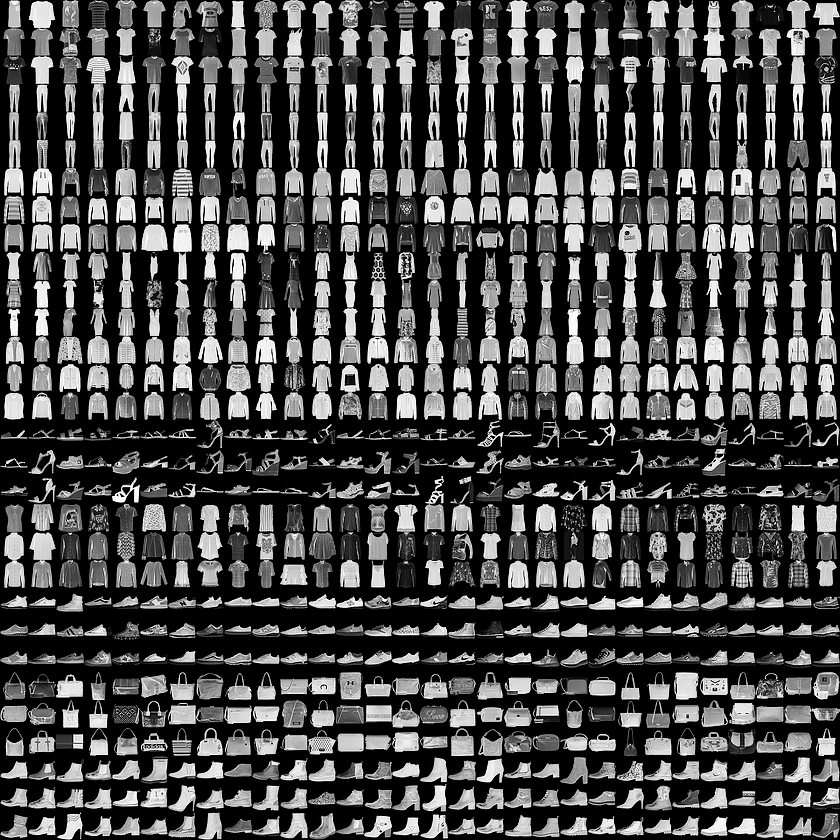
\includegraphics[width=\textwidth]{thesis_code/fashion-mnist-sprite.png}
	\caption{Examples from each class in the MNIST-Fashion Dataset. Each class is represented by three rows in the figure.}
	\label{fig:classifying_fashion-mnist}
\end{figure}

\subsection{Selecting a Convolutional Base}
\label{ssec:classifying_selectingbase}
Before turning to single-channel weather radar data in Section \ref{sec:classifying_zhcasa}, we must design an end-to-end model capable of matching or exceeding MNIST-Fashion benchmark error rates using a convolutional base trained initially on the ImageNet dataset.
There are several readily available models from which to choose \cite{chollet2015keras}.
It is assumed that in the well-trained case, a larger model corresponds to better generalization to unseen data, as there is more room within the architecture to model more features relevant to classification.
Meanwhile, smaller models may be have shorter training time necessitating less compute power, at the cost of generalization power.

To test this, we designed an experiment involving one well-known deep learning architecture from each category.
The VGG16 \cite{simonyan2014very} architecture represents a large model, at 528 MB, while MobileNet version 2 (MobileNetV2) \cite{sandler2018mobilenetv2} is much smaller, using 14 MB memory.
See Table \ref{table:classifying_conv_bases} for technical specifications of each model.

\begin{table}
\begin{tabular}{l r r}
	Model & Size & Parameters \\
	\hline
	VGG16 & 528 MB & 138,357,544 \\
	MobileNetV2 & 14 MB & 3,538,984 \\
\end{tabular}
\caption{Some relevant technical characteristics of two deep learning architectures}
\label{table:classifying_conv_bases}
\end{table}

Each convolutional base requires data to be formatted in a specific manner: input images must be normalized on the interval $[0,1]$; they must be a specific size, $[96 x 96]$; and they must contain three channels, since the convolutional bases were trained on three-channel RGB natural images.
In order to conform to these requirements, all training and testing images were generated from the dataset by a combination of upscaling the resolution and duplicating the single channel data to three channels, effectively retaining the black \& white input nature of the raw images.
At training and validation time, images were scaled from $[0,255]$ to $[0,1]$.
During training, data augmentation was utilized in an effort to "fake out" more data, as well as to attempt to make the network more generalizable to translations and scaling in the images.
Specifically, input images were centered and normalized, as well as randomly horizontally flipped.

We demonstrate the usage of each convolutional base using the same top model.
The top model uses as input the features extracted in each convolutional base, and learns to classify the target dataset using those features while training its own set of parameters.
Through theoretical and empirical processes, a relatively small top model consisting of 6 layers was chosen.
This set of layers includes batch normalization, global average pooling, dropout, dense connections, and its final output layer is a softmax classification layer.
An example diagram illustrating a top-down view of the end-to-end classifier is shown in Figure \ref{fig:classifying_architecture}.
During training, the weights in the convolutional base model are held constant, to preserve the findings from training on the ImageNet dataset and to provide the top model consistent inputs while it learns.
No fine-tuning was employed in this test.
Results of training can be found in Figure \ref{fig:classifying_conv_bases}.

\begin{figure}[ht]
	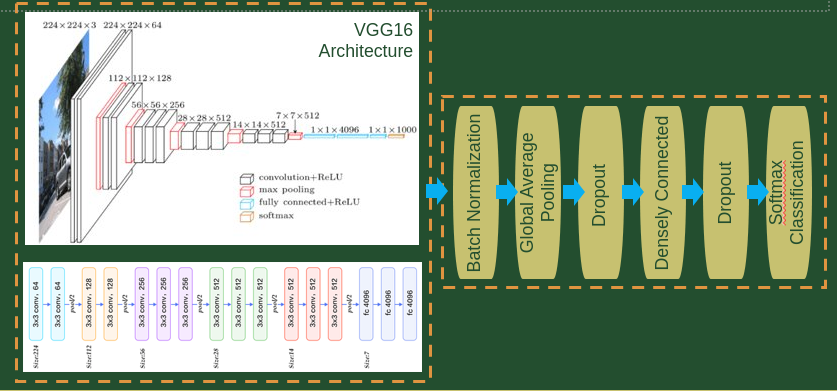
\includegraphics[width=\textwidth]{./thesis_code/vgg16_top_model.png}
	\caption{End-to-end deep learning architecture, with VGG16 convolutional base and bespoke top model.}
	\label{fig:classifying_architecture}
\end{figure}

\begin{figure}[ht]
	\centering
	\begin{subfigure}[b]{\textwidth}
		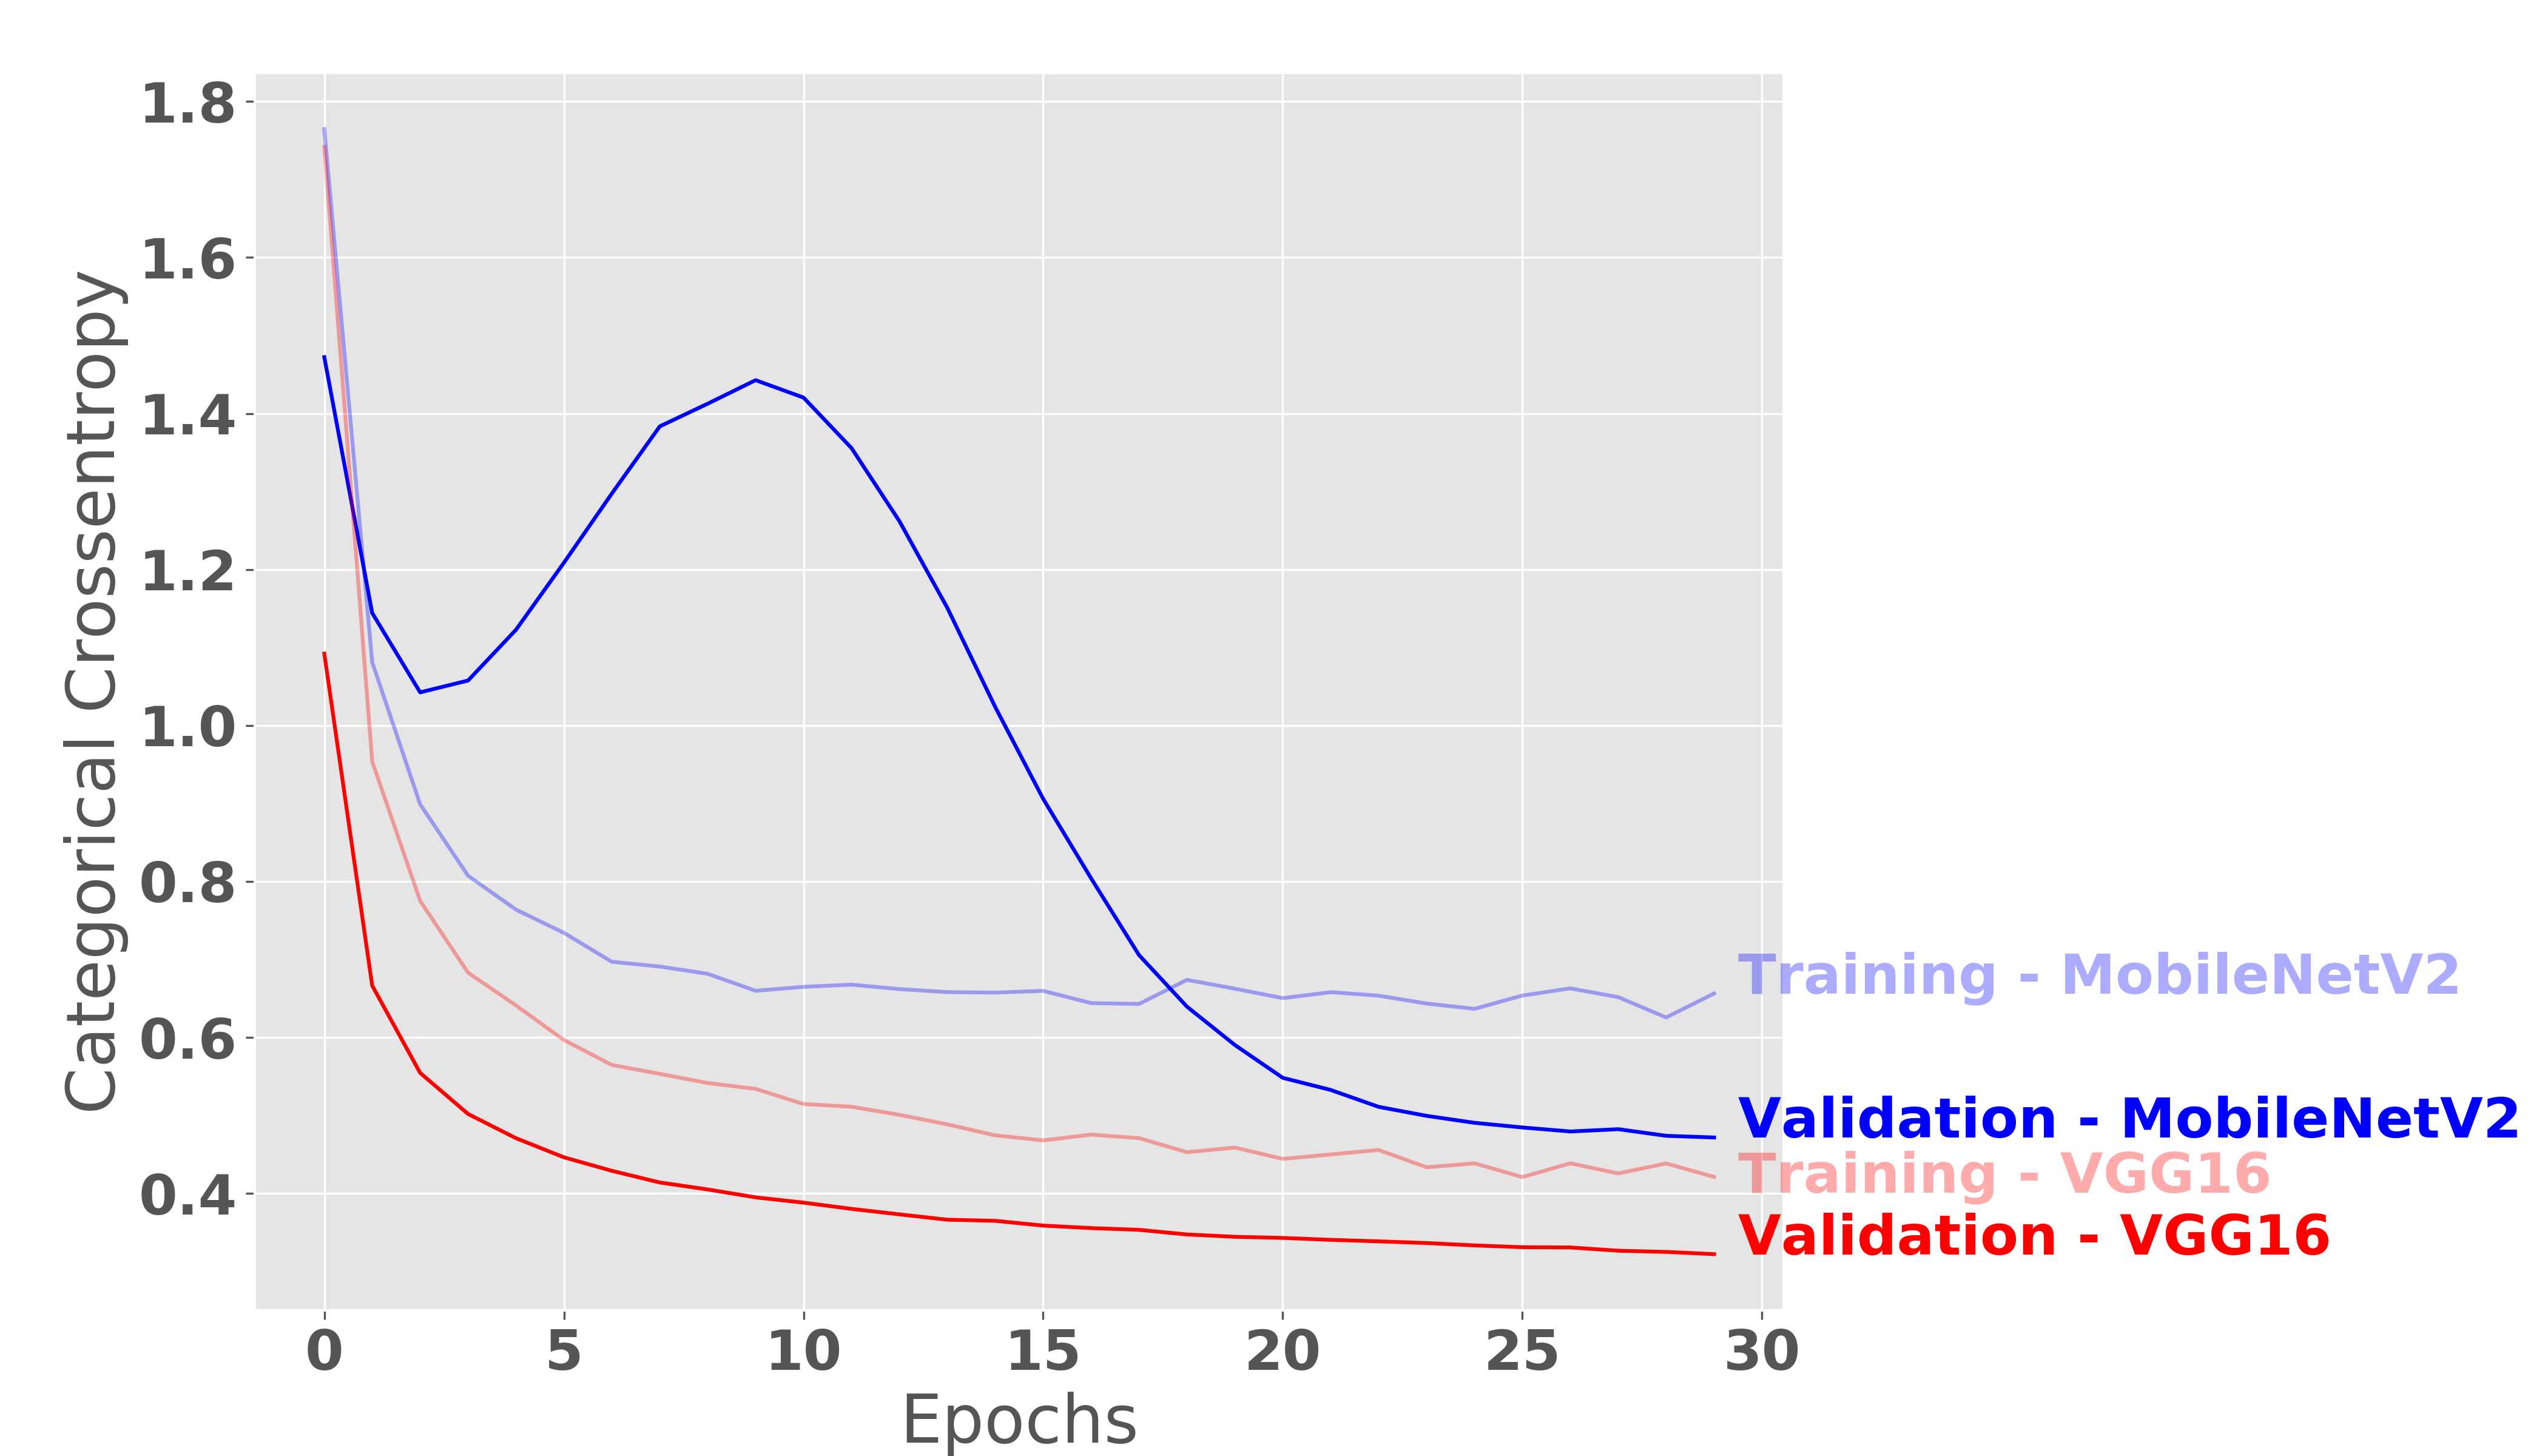
\includegraphics[width=\textwidth]{./thesis_code/plots/train-val-loss_two-nets_three-channels-duplicated.png}
		\caption{Loss}
		\label{fig:classifying_conv_bases_loss}
	\end{subfigure}
	\begin{subfigure}[b]{\textwidth}
		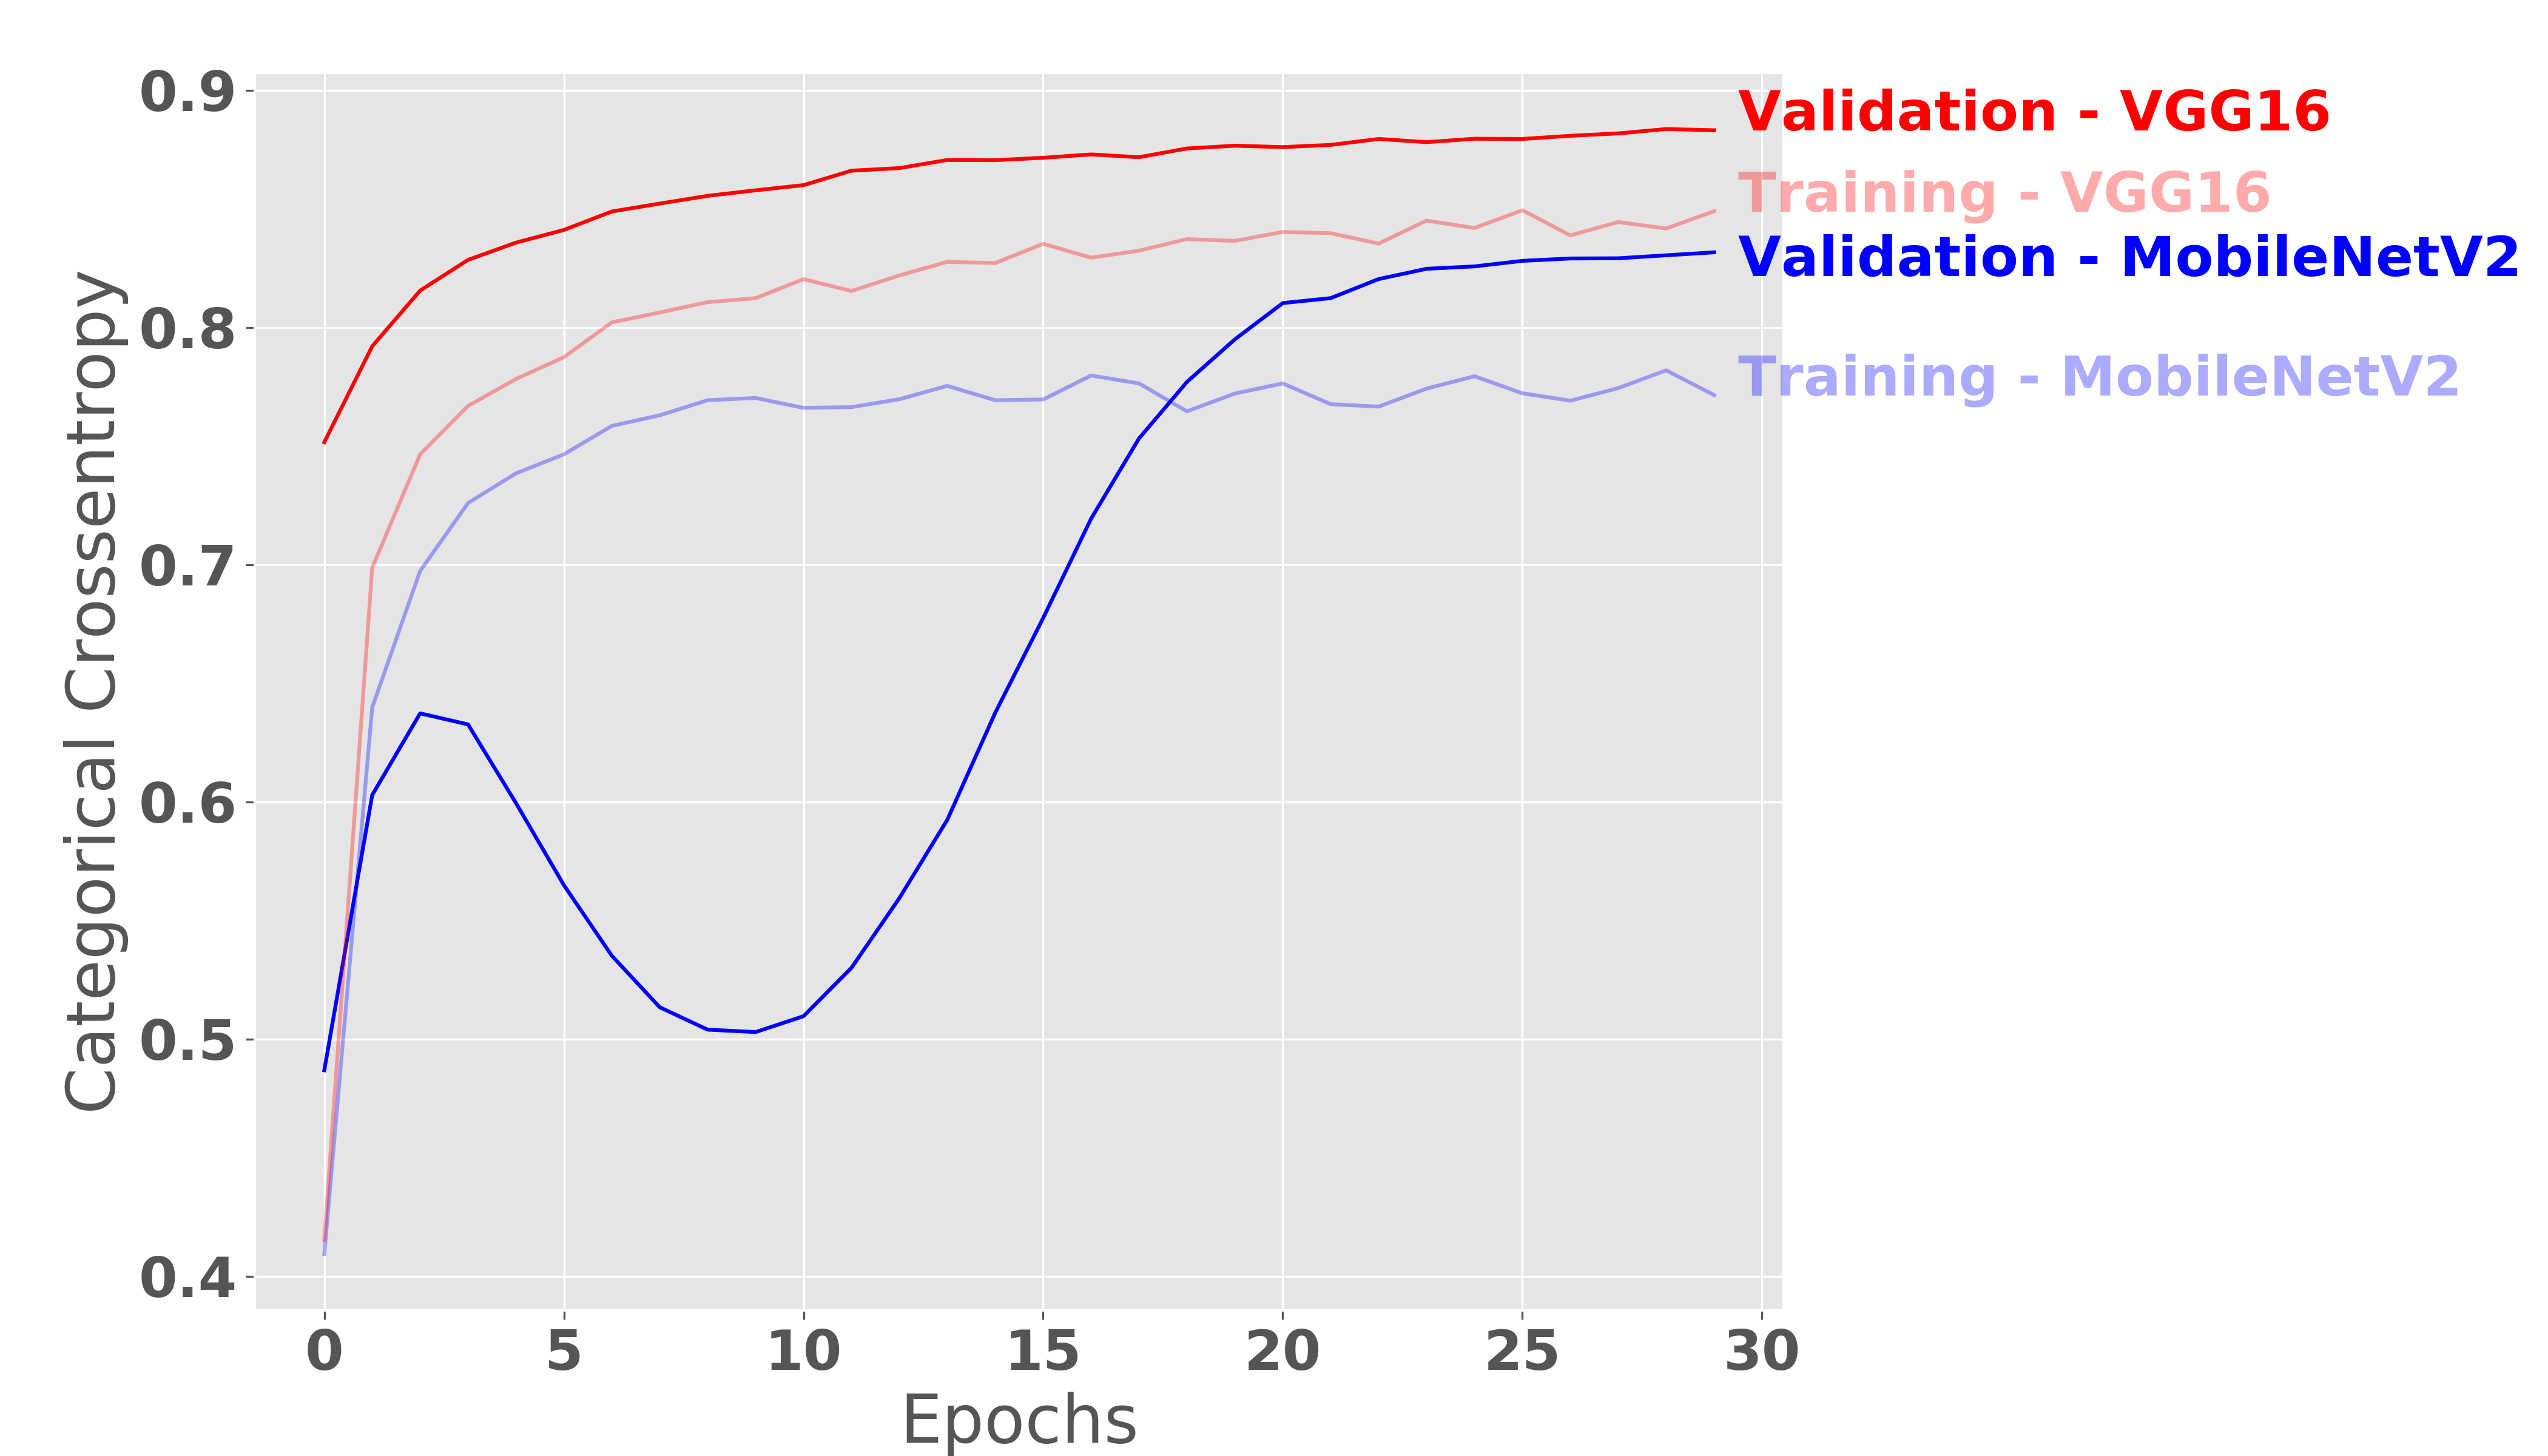
\includegraphics[width=\textwidth]{./thesis_code/plots/train-val-acc_two-nets_three-channels-duplicated.png}
		\caption{Accuracy}
		\label{fig:classifying_conv_bases_accuracy}
	\end{subfigure}
	\caption{VGG16 and MobileNetV2 training and validation characteristics during training on MNIST-Fashion dataset.}
	\label{fig:classifying_conv_bases}
\end{figure}

The results are interesting. Training was limited to 30 epochs, and while the loss had not completely leveled off at epoch 30, the results indicate that on the validation set, the VGG16-based model had a lower loss than the MobileNetV2 version.
This is in line with expectation, as the MobileNetV2 is intended as a valuable tool in performing classification on systems of limited compute power, but such limitations inhibit its ability to approach the accuracy found in larger models.
As such, the analysis in this work will focus on utilizing VGG16 as the convolutional base in classifying weather radar data.

Additionally, there is a region of interest with respect to the training characteristics of the MobileNetV2 model, where validation loss increases while training loss decreases.
It is unclear why this occurs in early epochs, though it is likely due to early overfitting when the smaller model perhaps memorizes the dataset.
Interestingly, this phase ends around epoch 10, where validation loss begins to decrease again and ultimately crosses the training loss.

That validation loss is lower than training loss at the end of training may seem to be counterintuitive, since the validation data is unseen when training batches.
However, this is not an uncommon result when using data augmentation in training.
The validation images are drawn from a held-out portion of the training dataset, but during validation, no data augmentation techniques are applied.
Thus, the model can perform better on validation data than the augmented training data, even while said augmentation assists in learning more generalized filters for the images.

Finally, we will see that validation accuracy, when using VGG16 as the convolutional base, can be increased.
Meanwhile, test set accuracy will match current available benchmarks, but in order to achieve this result, the entirety of the convolutional base will need to be made trainable, and many more epochs of training must occur.

\subsection{Does Colormap Matter?}
\label{ssec:classifying_colormap}
% Discussing importance of colormap in informing classifications, if there is any.
% Three tested: Black & White (3 channels duplicated), Viridis (perceptually uniform), NWS Reflectivity (segmented colormap to match weather radar)

Many weather radar variables, such as horizontal reflectivity $Z_h$, are intensity values.
In other words, there is some range of acceptable values from a minimum to a maximum value, and higher values indicate more intense or higher returns than lower values.
This is somewhat analogous to the type of data in the images in the raw MNIST-Fashion dataset, and as such, similar processing can be applied to the latter dataset to model the former.

Specifically of interest is the type of colormap used to visualize the data.
Weather radar data variables, when plotted as images, usually are represented by a mapping from their raw data space to a color space.
This mapping usually has some forethough behind it as well: radial velocity data, which ranges from a negative to positive Nyquist velocity of scatterers, centered about zero, is typically plotted using a diverging colormap; meanwhile, horizontal reflectivity, where higher values indicate larger and more intense precipitation, is plotted with a segmented colormap where "warmer" colors (i.e, red, orange, purple, white) identify higher returns than color colors (i.e, blue, green, etc).
When such a colormap is applied to data, the values are essentially quantized according to pre-determined bins.
Since $Z_h$ is in dB and since each increase in dB corresponds to an order of magnitude increase in power return of scatterers, these bins are usually kept to a small width; often, 4 dB width to a color, or perhaps "category," of reflectivity returns.
This is designed to inform human viewers as to the contents of the data and the type of scan, but encodes a large amount of potential values and cases in each bin.
Furthermore, such quantization represents a downsampling, so that images of weather radar data have less information than is present in the raw data.
Finally, textures present from this colormapping process in the processed images may represent artificial bounds, relatively arbitrary distinctions leveed upon continuous data.

The above factors raise concern in using pre-generated weather radar data as inputs to a classification model.
As data discovery is a fundamental goal of this research, and as many radar data servers continue to produce colormapped data of this type, it is imperative to discover if such operations impact the classification ability of a deep learning model.
We designed an experiment where the MNIST-Fashion data was colormapped according to three categories to test this:

\begin{enumerate}
	\item Pure Intensity (No colormapping): This is equivalent to the data that was used as input for the above experiment in determining the convolutional base to use
	\item Perceptually Uniform Intensity (Viridis): There has been growing interest\cite{kovesi2015good} in utilizing colormaps designed to appear continuous for human viewers in faithfully representing continuous data, as changes in color appearance can more accurately represent the changes in numerical data. 
	The viridis colormap can be found in many analysis packages in many languages (python\footnote{\url{https://matplotlib.org/gallery/color/colormap_reference.html}}, 
	MATLAB\footnote{\url{https://www.mathworks.com/help/matlab/ref/colormap.html}, listed as 'parula'}, 
	R\footnote{\url{https://cran.r-project.org/web/packages/viridis/index.html}}) and is chosen to represent this class of colormaps.
	\item Segmented Colormap (NWS Reflectivity): The National Weather Service uses a consistent colormap for reflectivity data, similar to the above, where warmer colors indicate higher returns, and cooler colors represent lower return values. 
	This is available in many analysis packages, but this research utilized the Py-ART package\cite{helmus2016python} 'NWSRef'\footnote{\url{http://arm-doe.github.io/pyart/dev/dev_reference/graph.html?highlight=nwsref}} colormap for this experiment.
\end{enumerate}

Refer to Figure \ref{fig:classifying_mnist-fashion_colormaps} for example images from three image classes, represented by each of the colormaps in this experiment.

\begin{figure}[ht]
	\centering
	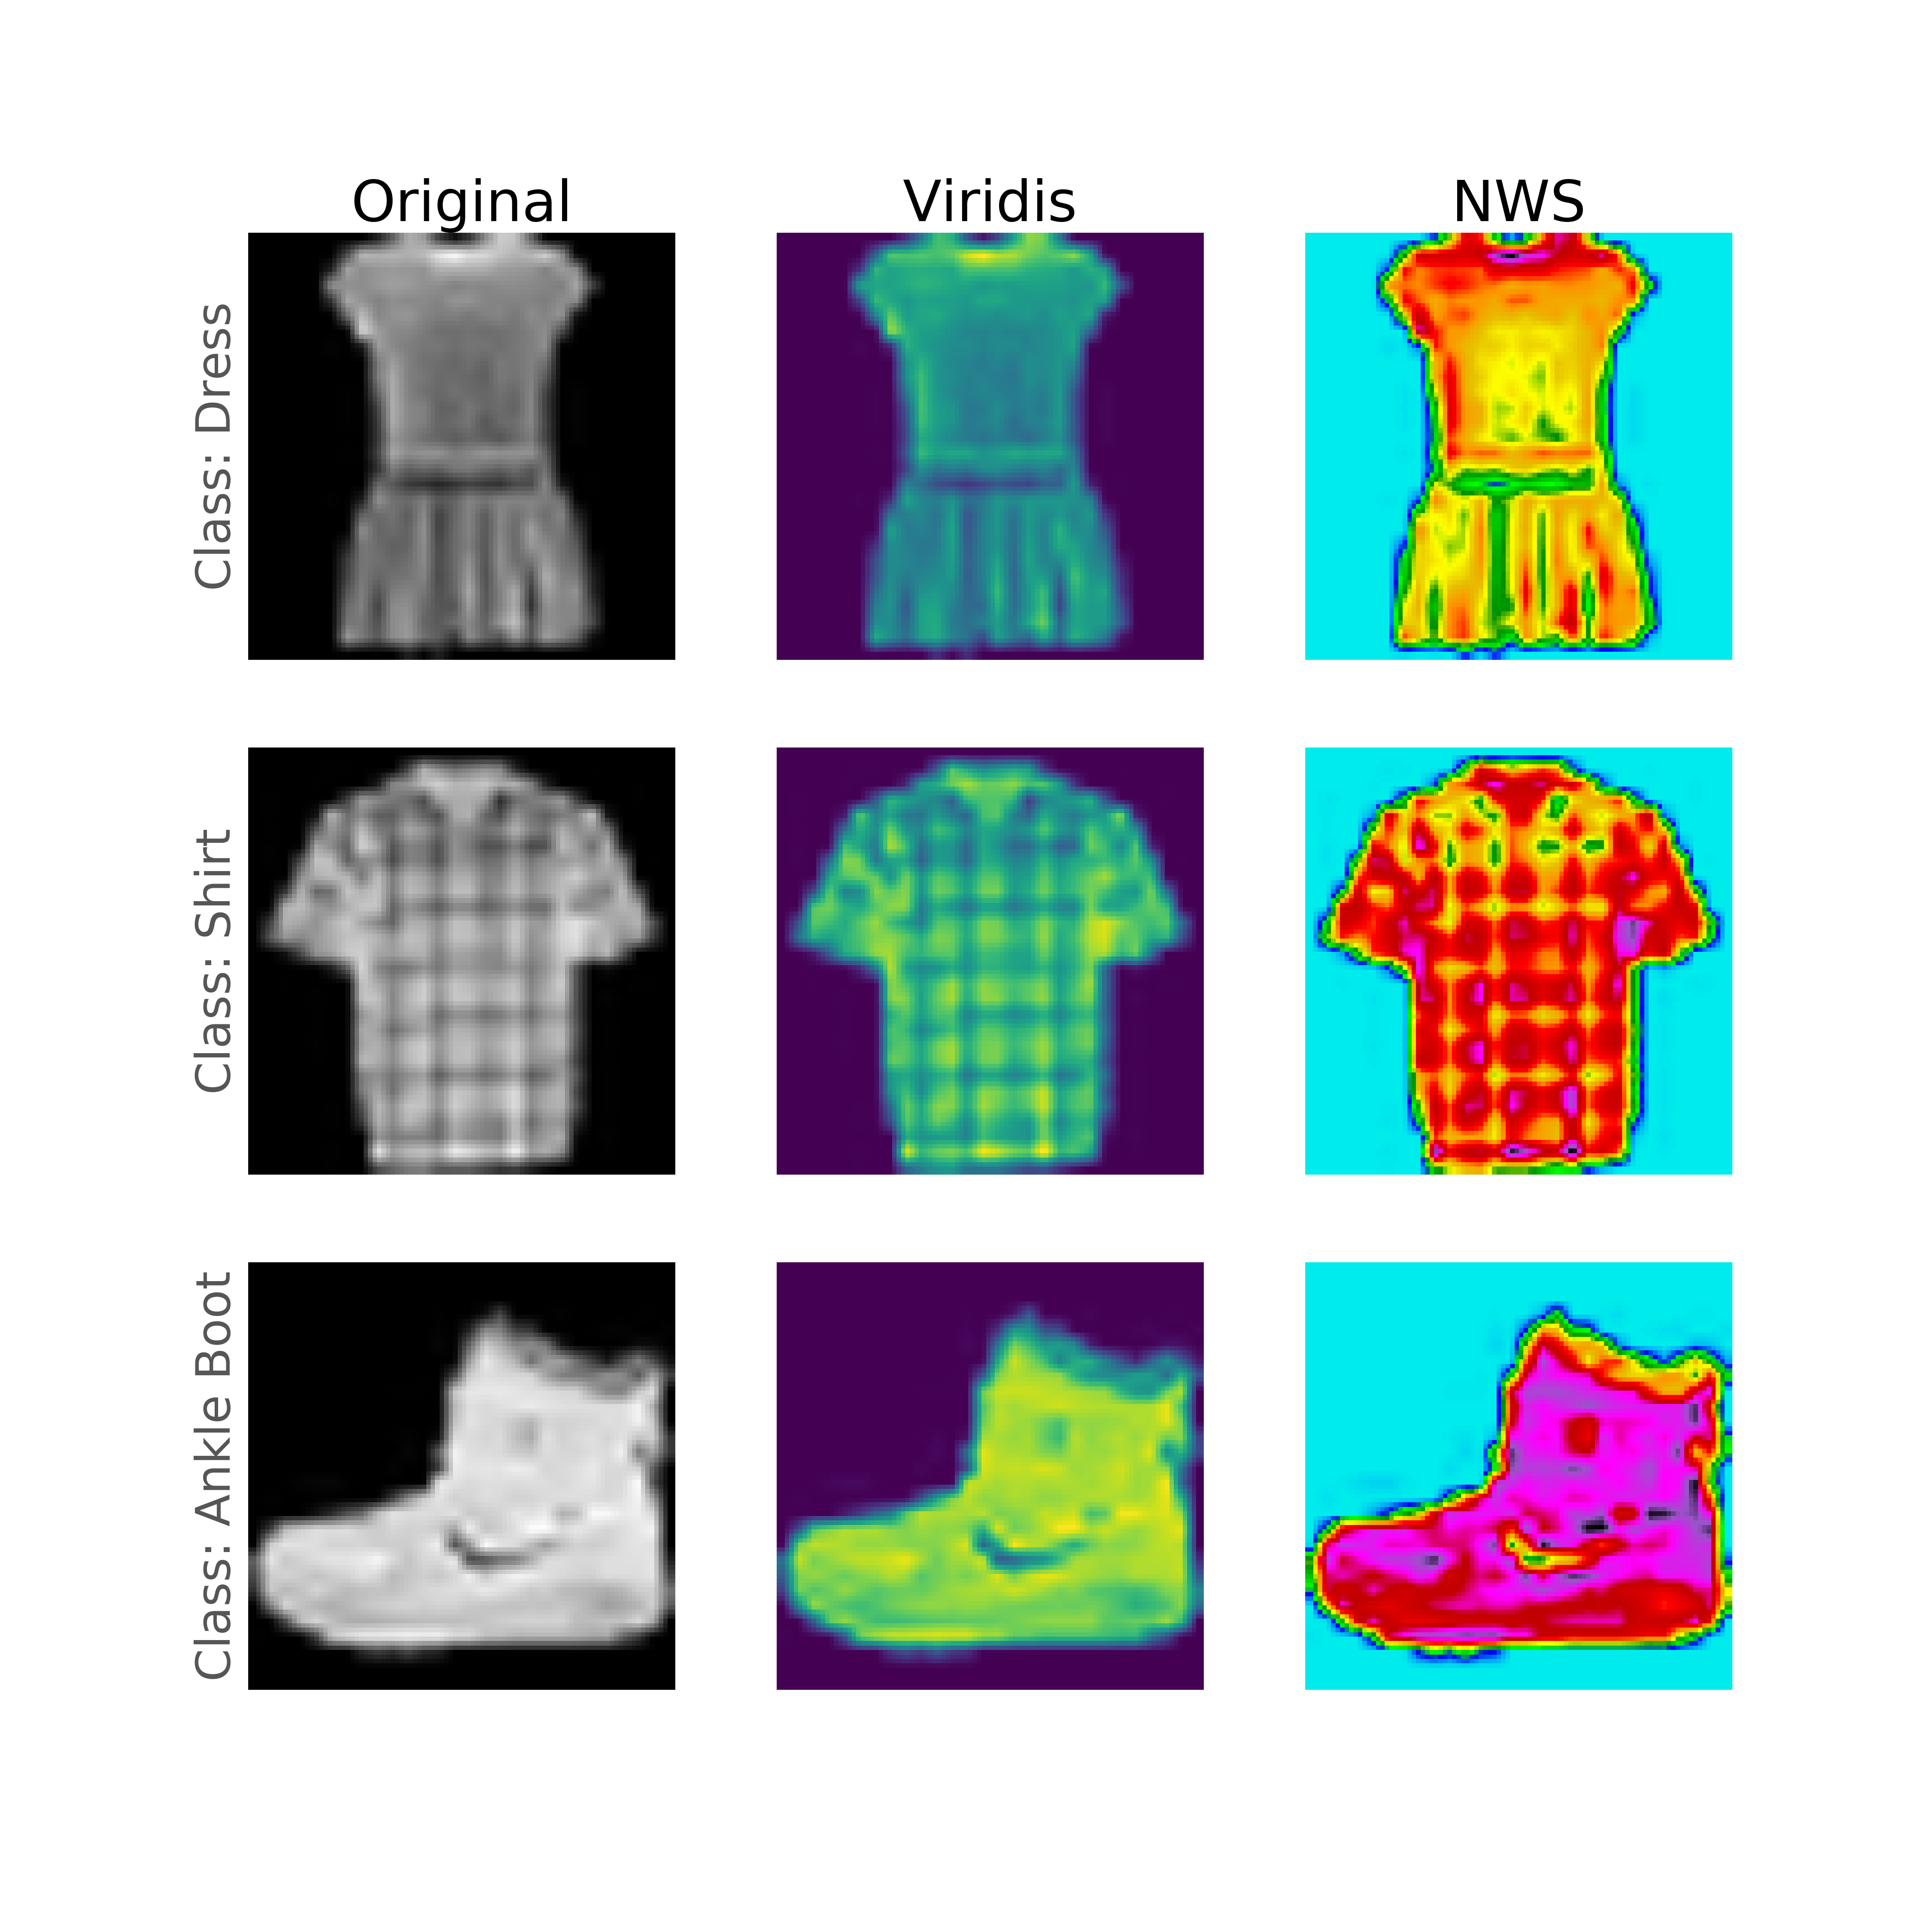
\includegraphics[width=\textwidth]{./thesis_code/plots/mnist_fashion_examples_colormapped.png}
	\caption{Various images from MNIST-Fashion dataset, visualized using different colormaps. Images appear blurry as they are resampled versions low-resolution ($[28 x 28]$) inputs.}
	\label{fig:classifying_mnist-fashion_colormaps}
\end{figure}

The deep learning model described above was trained and validated separately using each colormap for 30 epochs of training. 
As above, training data was augmented by random transformations chosen from pre-determined parameters.
The training and validation characteristics are shown below in Figure \ref{fig:classifying_colormaps-short-training}.

\begin{figure}[ht]
	\centering
	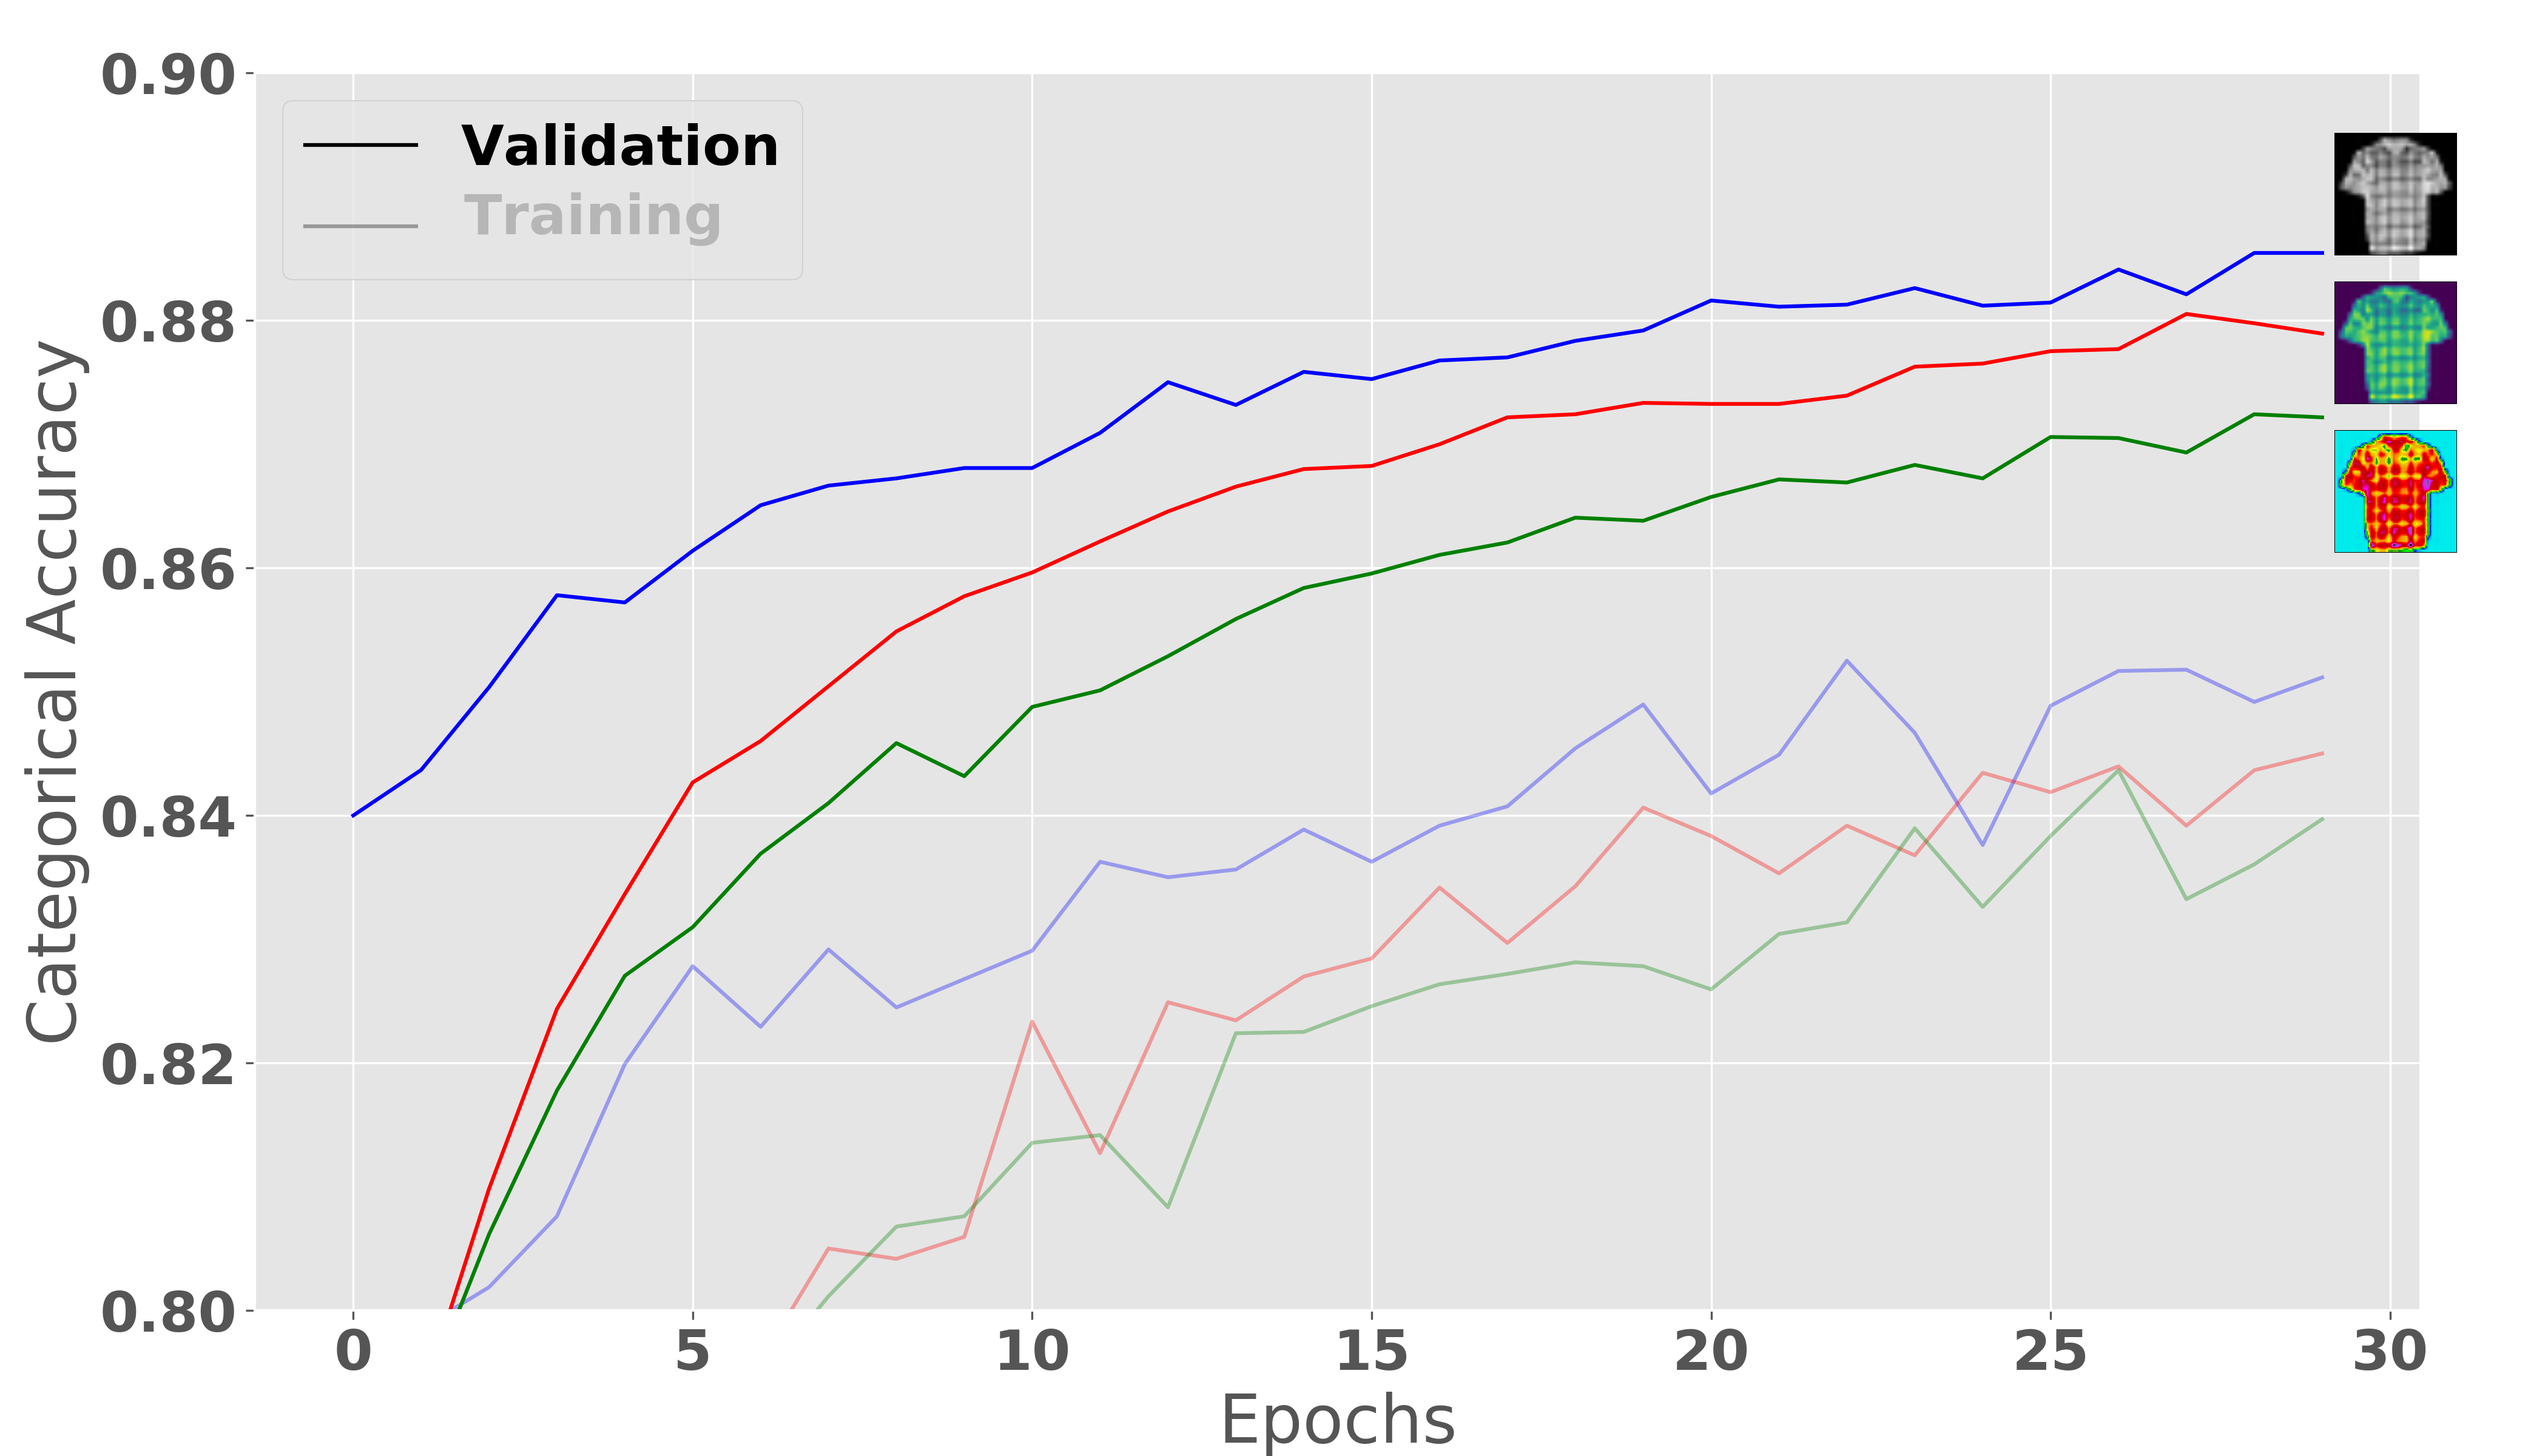
\includegraphics[width=\textwidth]{./thesis_code/plots/train-val-acc_colormaps.png}
	\caption{First 30 epochs in training deep learning model, with input image representations derived from three colormaps, black \& white, viridis, and NWS Reflectivity}
	\label{fig:classifying_colormaps-short-training}
\end{figure}

As before, we see that validation accuracy is higher than training accuracy, while validation loss is lower than training loss, as can be seen when data augmentation is used in training.
This plot shows better results for the data in its original format, with each input channel corresponding to the same intensity values, which renders as a black \& white image.
The viridis colormapped data shows the next best results, followed by the NWS Reflectivity data.
However, it is important to note that at this point in training, each validation accuracy continues to rise.
As such, we should examine the results following a longer period of training, to find where each network learns as much as it can, with respect to classifying new data.

\subsection{Fine Tuning}
\label{ssec:classifying_finetuning}
% Fine tuning experiment to examine validity of this method in classifying data

As demonstrated in Figure \ref{fig:classifying_colormaps-short-training}, the network is able to learn data from each colormap and produce satisfactory validation accuracy results even after 30 epochs of training.
However, it is also apparent that longer training time will continue to increase the learning in the model, as none of the validation accuracy plots have reached a horizontal asymptote.
As such, we can continue training in the model for more epochs to see if the loss and accuracy continues to improve.
To assist in training, we monitor the validation loss, and if 10 epochs of training have passed without an improvement, the learning rate is reduced by a factor of 5.
The motivation for this is that each gradient step after each batch loss is computer is unable to further approach the local minima in the convex region of the multi-dimensional loss function, but that if the learning rate is lowered, gradient steps will be decreased, allowing further training.

Additionally, we employ a technique called \textit{fine tuning}, whereby after a set number of training epochs has reached, all layers in the convolutional base are unfrozen and the entire model is trained for a further number of set epochs.
The idea is that the features extracted in the convolutional base, as trained upon the natural images in ImageNet, are not as accurate on the target task as they could be, and so we must allow the weights in the base model to adapt to this target dataset through more training.
In order to not lose the insights learned when training the top model, however, we set the learning rate to a lower value, so that each gradient step does not drastically change the makeup of a framework that is already working well.

Other authors have attempted to find not only working methods for training such architectures, but to also find optimized versions.
In fact, this process is at the core of \textit{transfer learning}, which again, is the process by which a model is trained deeply and carefully on a source dataset, but is then adapted to a new target task.
Two works stand out from early in the development in this field: \cite{yosinski2014transferable}, which trained AlexNet \cite{krizhevsky2012imagenet} on a few different source tasks and tested on different target tasks; and \cite{oquab2014learning}, which was also based on AlexNet but replaced the final layer with two custom designed layers, making a top classifier to perform object detection on a different (but still natural image) dataset.
The latter stresses the importance of adding layers to assist the network learning to generalize to the new task, while the former illustrates that fine tuning as described above actually led to better results on a target dataset trained from source data, than a network simply trained on the target task in the first place.

The result of this is that we can implement these same concepts using larger networks, and expect to see good results.
To test this hypothesis, we employ the following strategy for each of the three datasets:

\begin{enumerate}
	\item Initialize weights in top classifier, freeze weights in convolutional base (VGG16)
	\item Compile model with adaptive learning rate technique Adam, initial learning rate = $1 x 10^{-4}$
	\item Begin training, 300 batches of size 32 original and augmented images per epoch, for 100 epochs
		\item If a validation set loss plateau is reached, reduce learning rate by factor of 5 and continue training
	\item After 100 epochs: 
		\item Unfreeze all layers in convolutional base
		\item Reset Adam learning rate to $1 x 10^{-5}$ 
		\item Continue training as above
	\item Stop training after a further 100 epochs (total 200)
\end{enumerate}

The goal of this experiment is in part to fundamentally understand that maximum learning capabilities of the end-to-end convolutional neural network model with respect to the various colormapped input datasets.
The results are shown in Figure \ref{fig:classifying_longtraining_finetuning} below.

\begin{figure}[ht]
	\centering
	\begin{subfigure}[b]{\textwidth}
		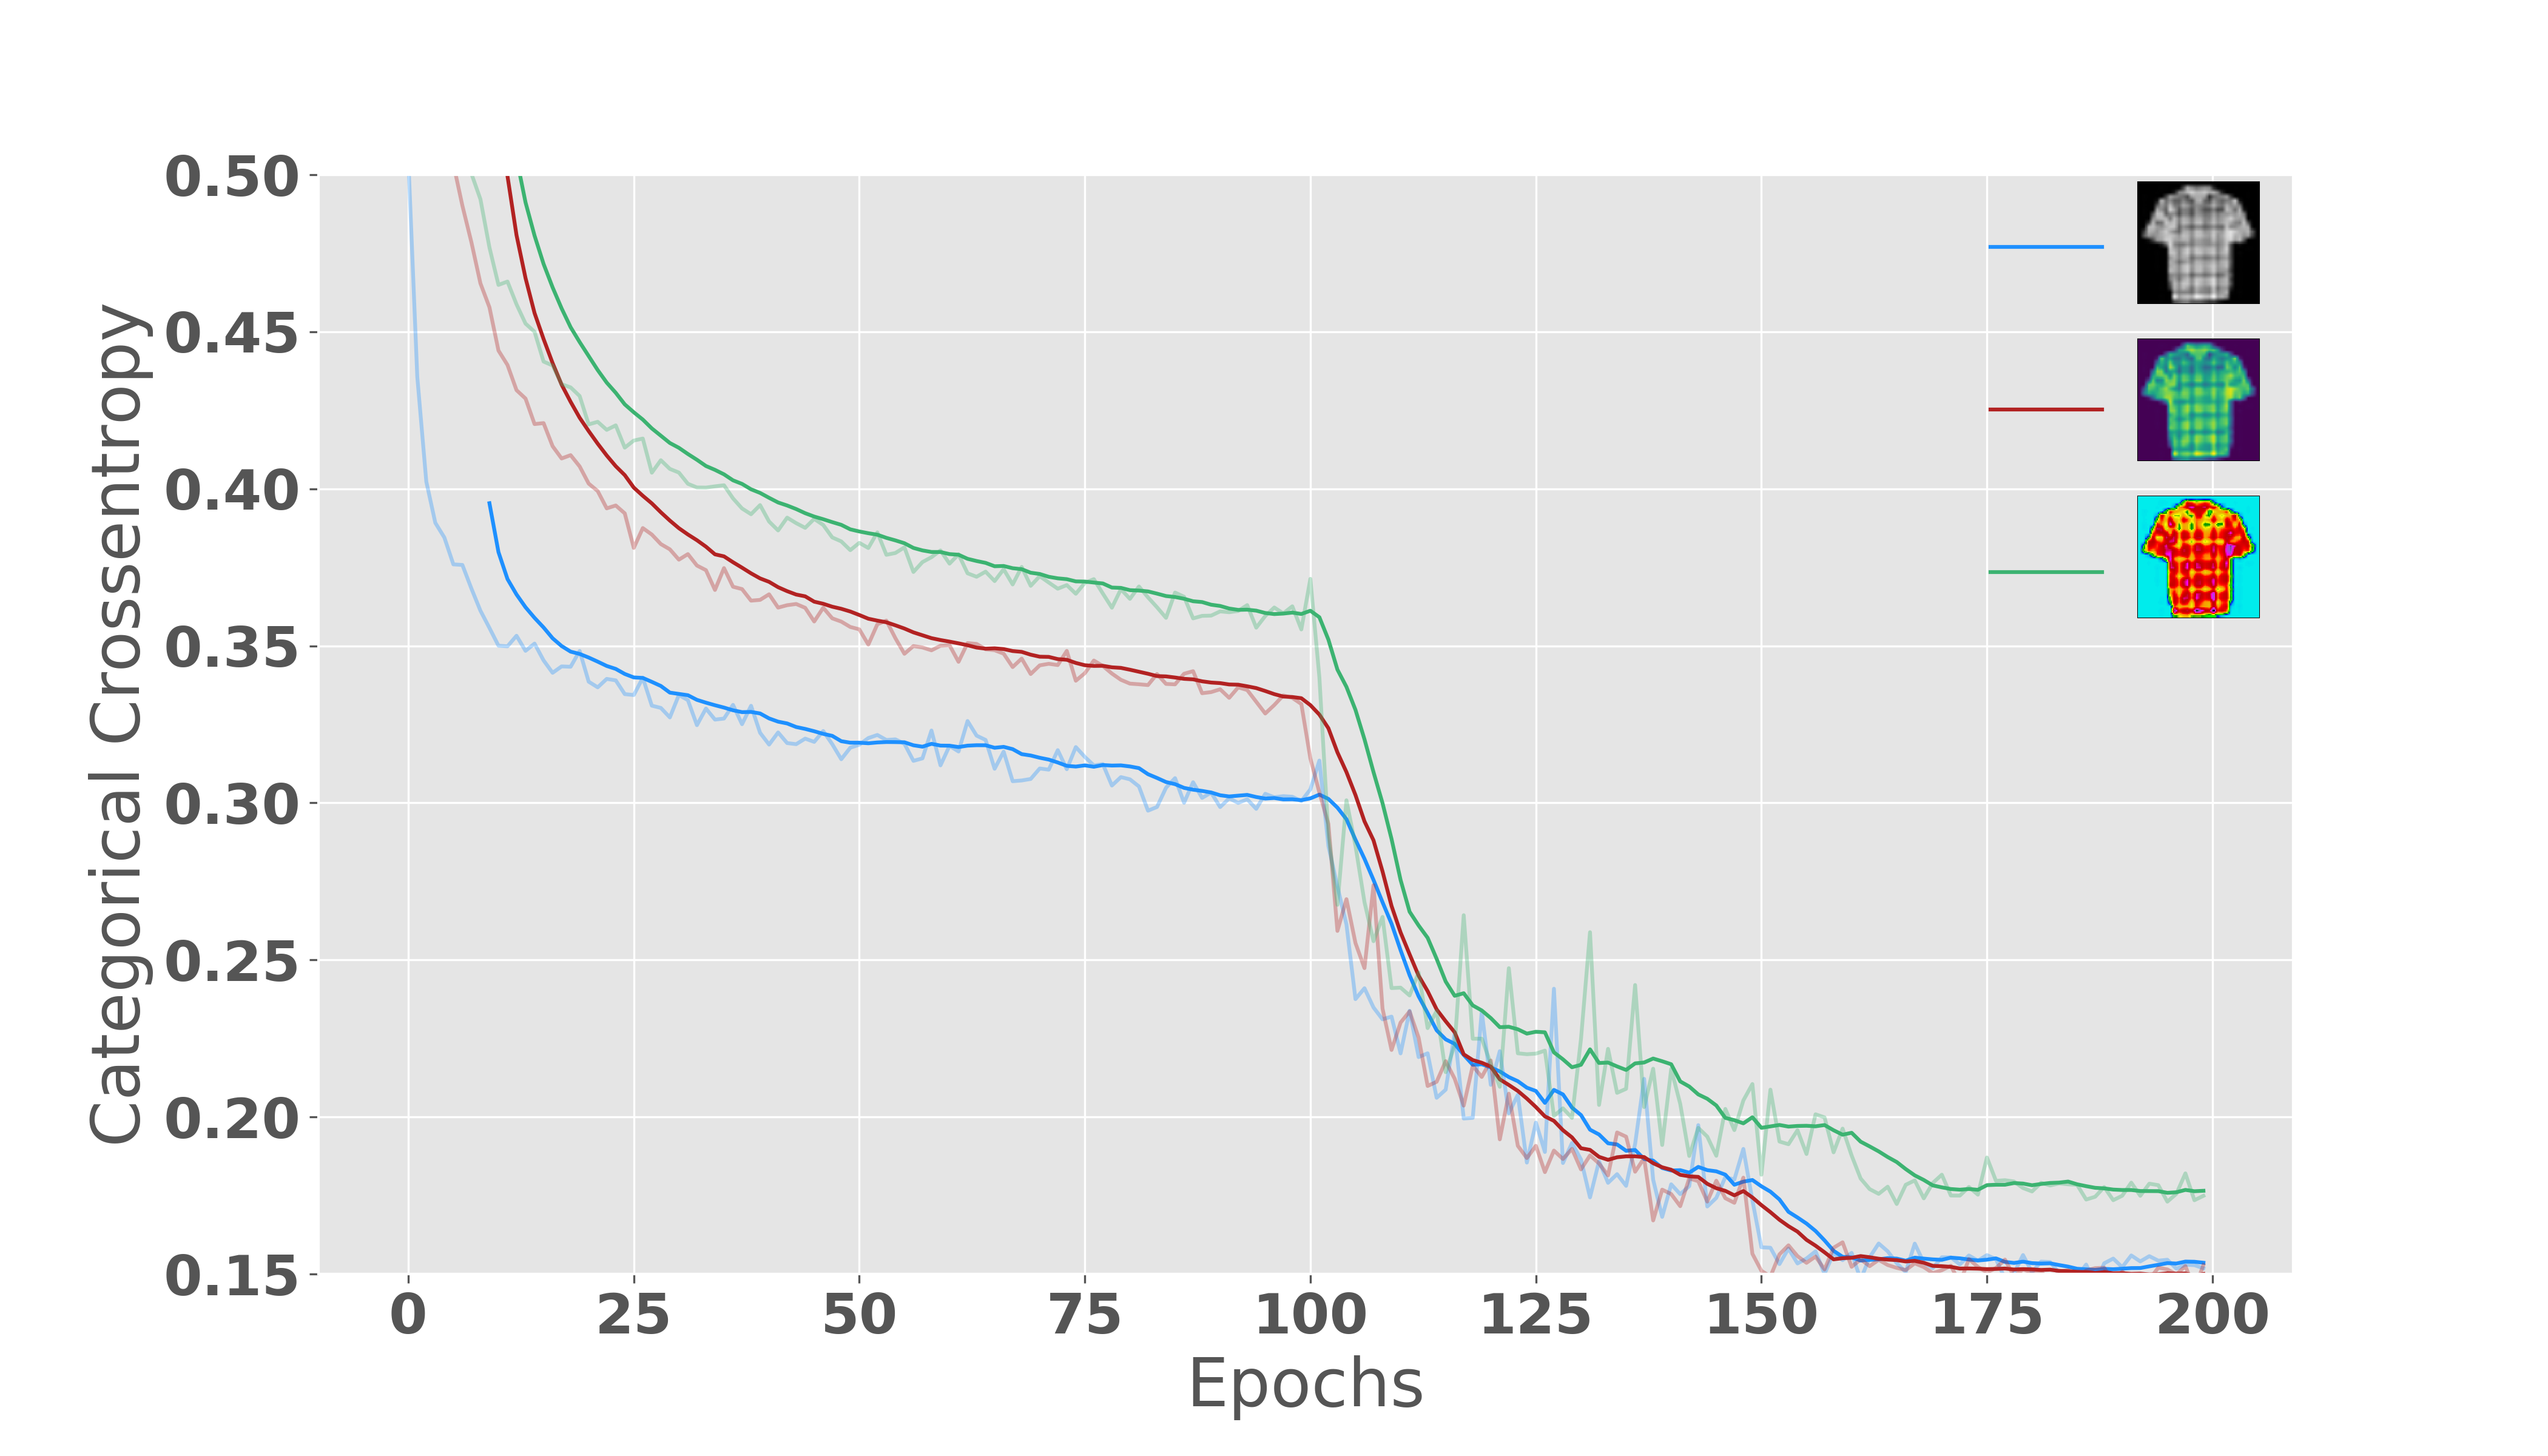
\includegraphics[width=\textwidth]{./thesis_code/plots/20190425_200epoch_finetuning_mnistfashion_loss.png}
		\caption{Loss}
		\label{fig:classifying_longtraining_finetuning_loss}
	\end{subfigure}
	\begin{subfigure}[b]{\textwidth}
		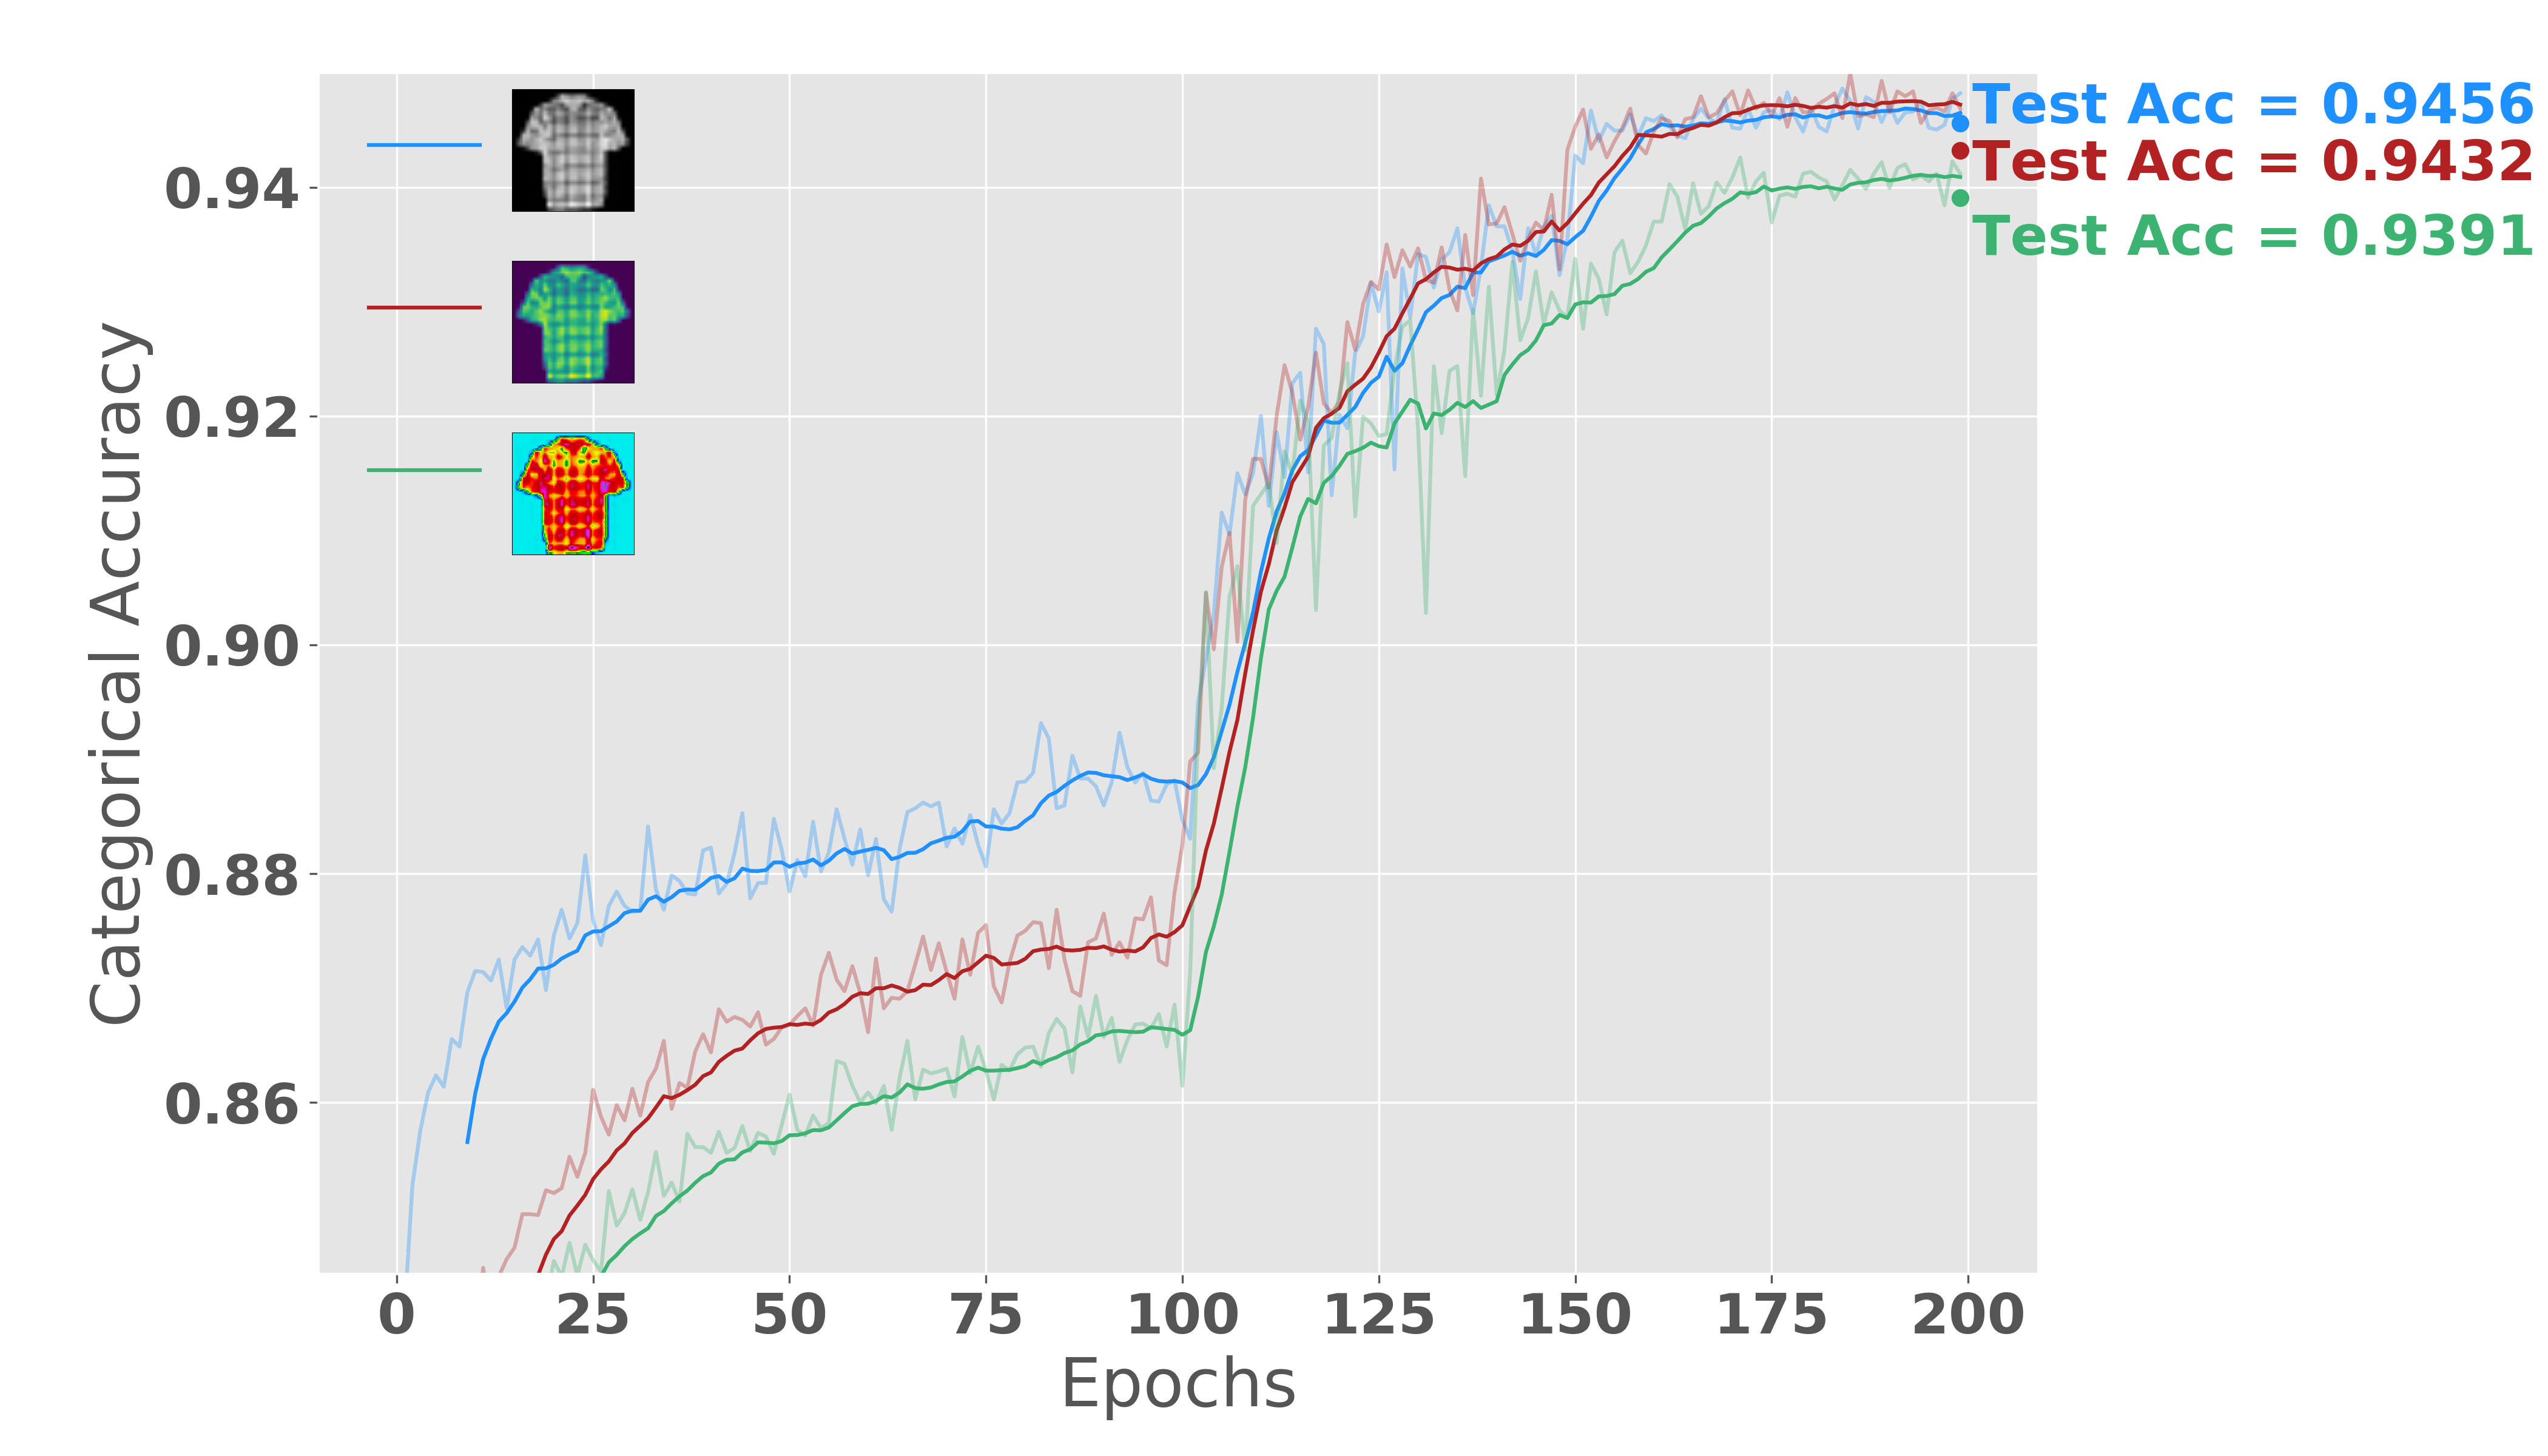
\includegraphics[width=\textwidth]{./thesis_code/plots/20190425_200epoch_finetuning_mnistfashion.png}
		\caption{Accuracy, with final test set accuracy as well}
		\label{fig:classifying_longtraining_finetuning_acc}
	\end{subfigure}
	\caption{Fully training \& fine tuning the VGG16 + top model classifier network on each dataset respectively, and computing learning characteristics. Interestingly, the NWS Reflectivity colormapped data works well, but not as well as both the original dataset, and the viridis colormapped data.}
	\label{fig:classifying_longtraining_finetuning}
\end{figure}

We would expect that the original data has the best results, followed by the colormapped sets, which artificially introduce color mappings to aid human viewing.
Additionally, we expect the NWS Reflectivity to suffer further deleterious effects due to its lower resolution binned color scale, which introduces artificial textures not present in the raw intensity data.
In fact, this is the case, though there are some interesting results to examine.
First, the perceptually uniform colormap, viridis, has nearly the same loss and accuracy curves in the fine tuning phase of training, as well as a similar test set accuracy.
This perhaps may indicate a utility in using perceptually uniform colormaps for not only human visualization but in machine learning settings as well.
Second, while the training characterization suffers when using the NWS Reflectivity colormap, the validation and test set accuracies are still quite good.
For the record, the best test set accuracy on the MNIST-Fashion dataset, using VGG16 as
convolutional base, is 0.935\footnote{\url{https://github.com/zalandoresearch/fashion-mnist}} as of this writing, which all three datasets surpass in this experiment.

The major takeaway here is that colormapped intensity data can provide a useful and satisfactory dataset for transfer learning.
We can have some confidence now, that the model will be able to learn and classify when considering radar data, many variables of which represent intensity values and which are often visualized in colormapped form.
This is particularly useful in the case of the CASA DFW data, which is stored not only in NetCDF form for the raw data, but also has pregenerated radar moments for each scan to assist in human viewing of historical data.
The experiments regarding this data, as well as its usage in classifying precipitation regimes, will be detailed in the next section.

\section{Classifying Reflectivity - CASA DFW}
\label{sec:classifying_zhcasa}

% Hand labeling data from Midlothian, separated into two classes, one for each precipitation regime, 
Data was hand-labeled by the author into one of three classes:

\begin{itemize}
	\item Stratiform Precipitation
	\item Convective Precipitation
	\item Unclassified
\end{itemize}

The first two were labeled when the conditions in Chapter \ref{sec:meteorology} were met for each case.
The third category is considered to be "everything else," for now.
Once these categories were populated, the model described above was trained using the reflectivity pre-generated images as inputs.
The data was split into a training and testing set, where each were about 3 same size, and the testing set was populated with data from completely different days than in training.
When training, the data was further split into two sets, where 90\% of the training set was actually input to the model, and the remaining 10\% was used for computing validation characteristics during training.
It was by monitoring the validation loss and categorical accuracy that we were able to employ an early stopping condition in training, in order to avoid overfitting.
Due to the small size of the dataset, this occurred after only 15 epochs of training.

We must detail a few success metrics here in order to compare the results of this experiment to similar ones described in Chapter \ref{sec:meteorology}.
There are five metrics listed in \cite{anagnostou2004convective}, which we formulate here and compare to the results observed in the present experiment.

Probability of detection (POD) is given by:

\begin{equation}
\mathrm{POD} = \frac{n_{true positive}}{n_{true positive} + n_{false negative}}
\end{equation}

False alarm rate (FAR) is given by:

\begin{equation}
\mathrm{FAR} = \frac{n_{false positive}}{n_{true positive} + n_{false positive}}
\end{equation}

Cumulative success index (CSI) is given by:

\begin{equation}
\mathrm{CSI} = \left[\left(\mathrm{POD}\right)^{-1}+(1-\mathrm{FAR})^(-1)-1\right]^{-1}
\end{equation}

The results from this experiment are detailed in Table \ref{table:classifying_zh_comparison} below. 
The two final parameters from the original paper\cite{anagnostou2004convective} are omitted as they relate to pixels, not only precipitation regime.
Furthermore, the deep neural network presented here (DNN) was trained on a third class to be able to ignore images that were unrelated to stratiform or convective precipitation, which was not performed by the other methods.
As such, we add a third entry to the table below.

\begin{table}
	\begin{tabular}{l l r r r }
		Algorithm & Rain Type & POD & FAR & CSI \\
		\hline
		NN\cite{anagnostou2004convective} & Stratiform & 0.97 & 0.07 & 0.90  \\
		   & Convective & 0.52 & 0.29 & 0.43  \\
		SHY95\cite{steiner1995climatological} & Stratiform & 0.85 & 0.05 & 0.81  \\
		      & Convective & 0.72 & 0.59 & 0.36  \\
		BL00\cite{biggerstaff2000improved} & Stratiform & 0.84 & 0.04 & 0.80  \\
		     & Convective & 0.74 & 0.58 & 0.36 \\
		SHYM\cite{anagnostou2004convective} & Stratiform & 0.89 & 0.05 & 0.85  \\
		     & Convective & 0.69 & 0.51 & 0.40 \\
		\hline
		DNN & Stratiform & 1.00 & 0.00 & 1.00 \\
		    & Convective & 0.99 & 0.04 & 0.96 \\
		DNN & \textbf{Overall} & \textbf{0.976} & \textbf{0.012} & \textbf{0.965} \\
	\end{tabular}
	\caption{Statistics for various algorithms in the literature in calculating stratiform and convective precipitation regimes. The algorithm presented in this research is denoted by DNN, and includes a third class to model all other cases. As such, a row is reported illustrating the overall classification rates, and is bolded to emphasize this.}
	\label{table:classifying_zh_comparison}
\end{table}

\subsection{Data Discovery}
\label{ssec:classifying_discovery}

Deploying the model on CASA DFW servers as a way to identify candidate scans for enlarging precipitation regime dataset, and using iterative, semi-human-supervised process to expand dataset.
Given the complicated nature and lack of conviction regarding directory structural conventions, the CASA DFW servers are particularly challenging to parse.
However, this is a data engineering problem.

As a substitute, several directories were backed up locally to allow deployment of the model and general testing to occur.
The trained model was deployed on two months of data: June 2018 and September 2018. 
For June, convective precipitation was identified, while no stratiform scans were selected.
This is perhaps to be expected, given the warmth in the Dallas-Fort Worth area in the peak summer months, and a higher likelihood of convective activity.
Some sample scans identified are shown below.

\begin{figure}[ht]
	\centering
	\begin{subfigure}[b]{0.45\textwidth}
		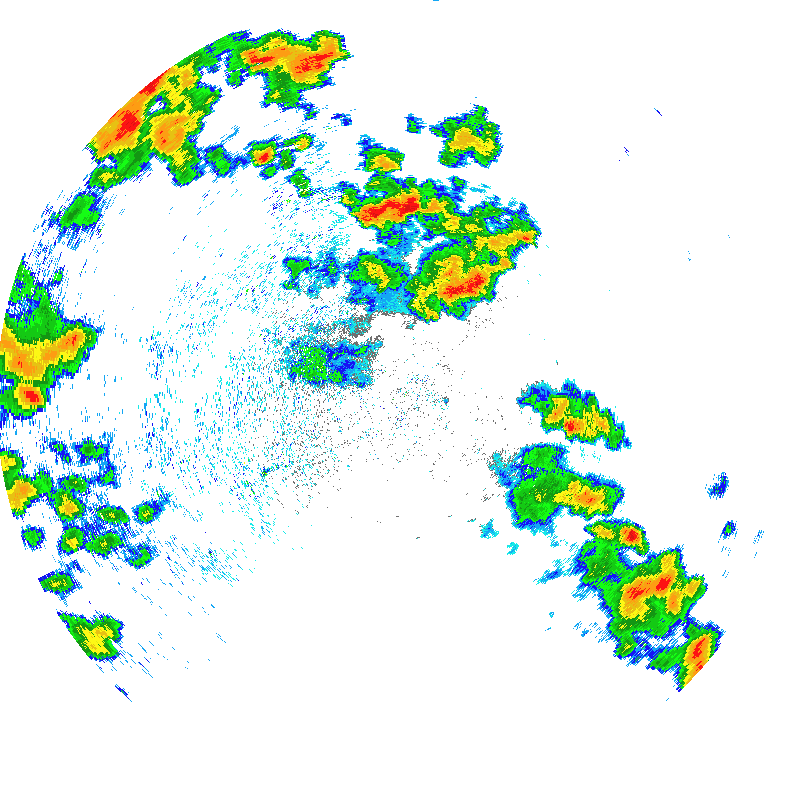
\includegraphics[width=\textwidth]{./thesis_code/plots/midlothian-tx-20180604-115830-ref.png}
		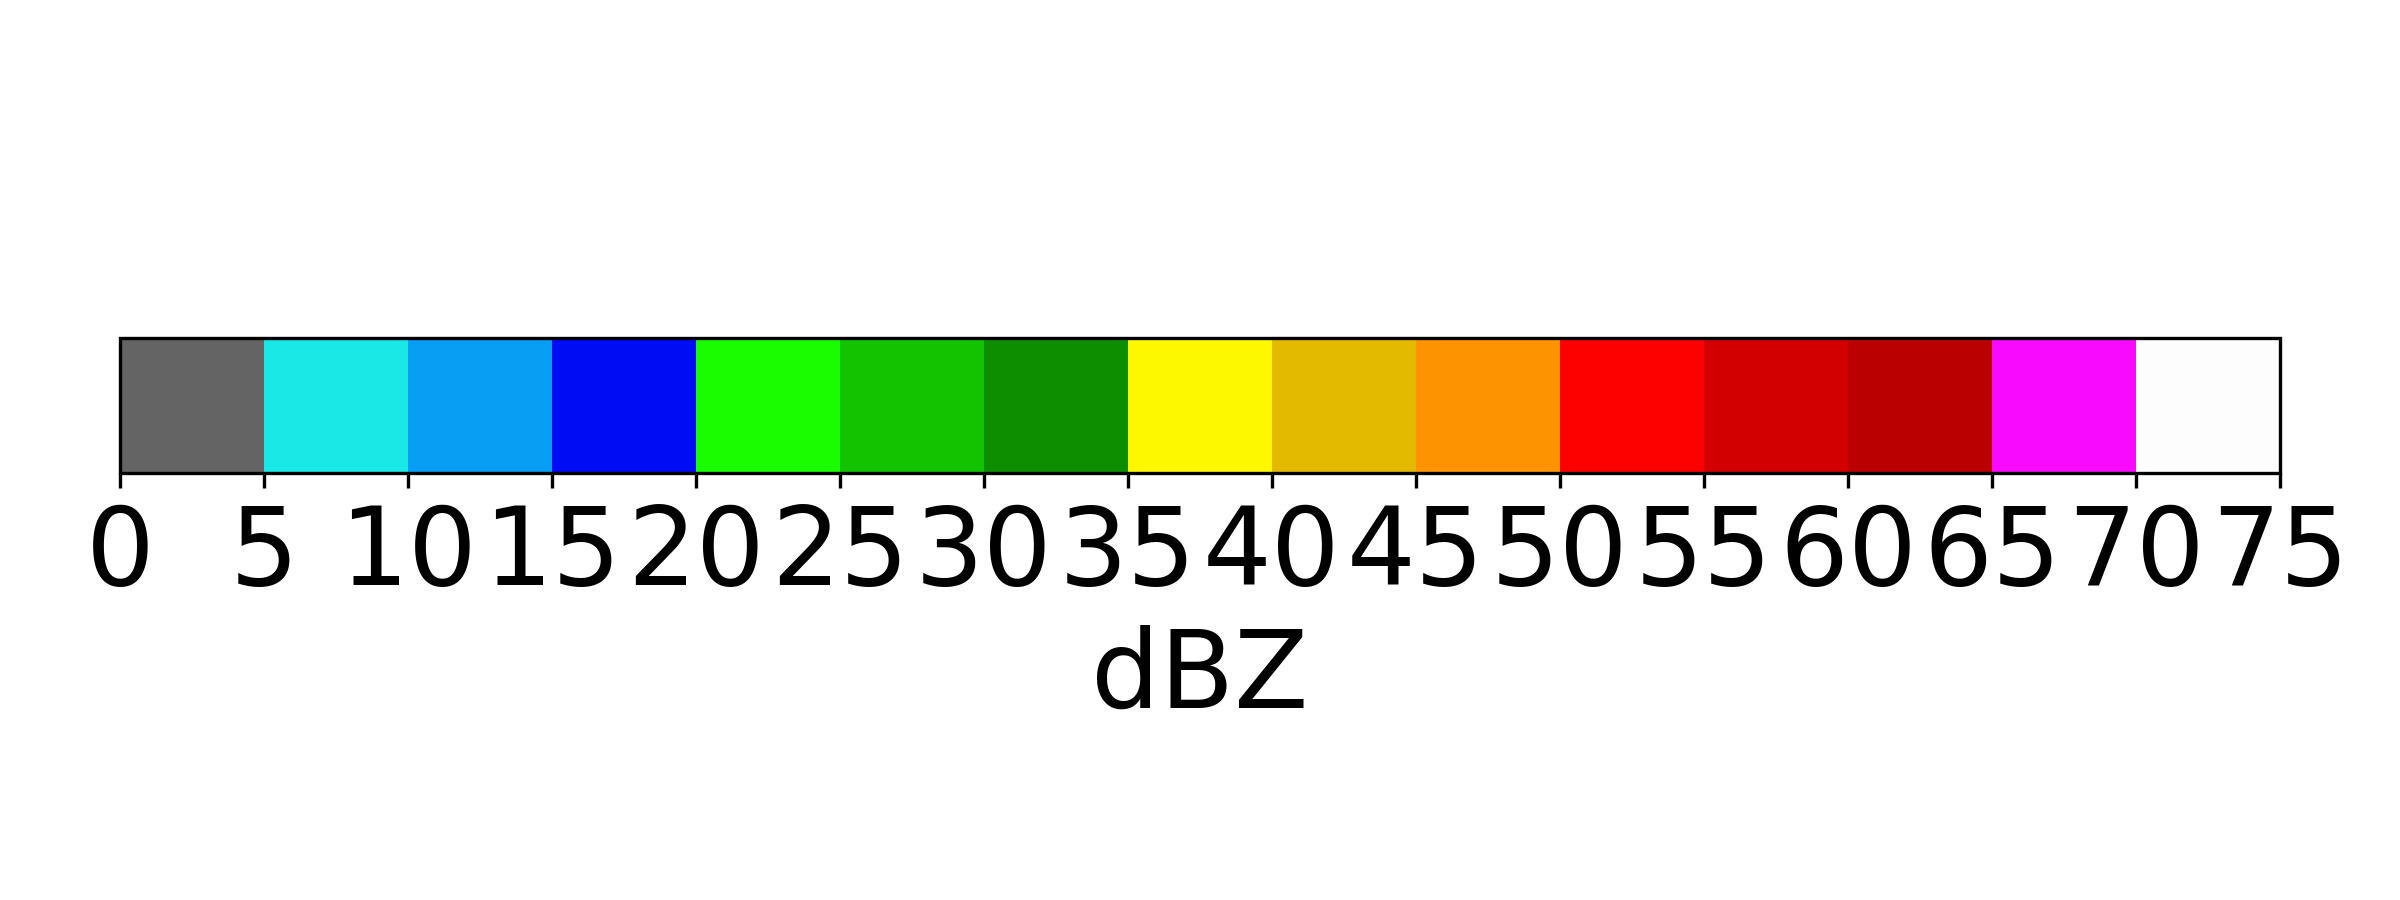
\includegraphics[width=\textwidth]{./thesis_code/plots/dfw_colormap.png}
		\caption{20180604}
		\label{fig:classifying_datadiscovery_ex1}
	\end{subfigure}
	\begin{subfigure}[b]{0.45\textwidth}
		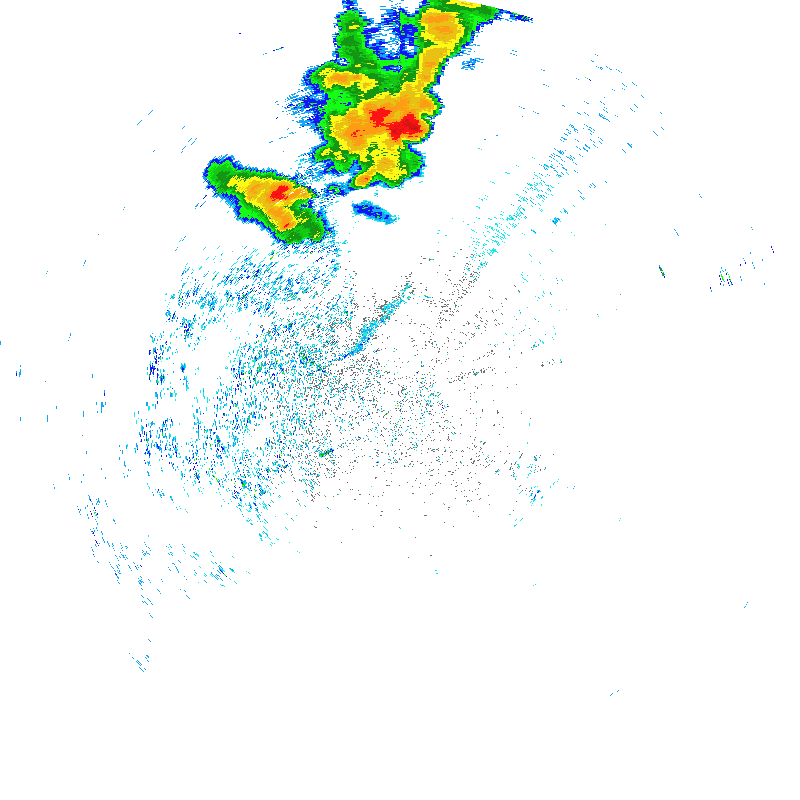
\includegraphics[width=\textwidth]{./thesis_code/plots/midlothian-tx-20180607-233029-ref.png}
		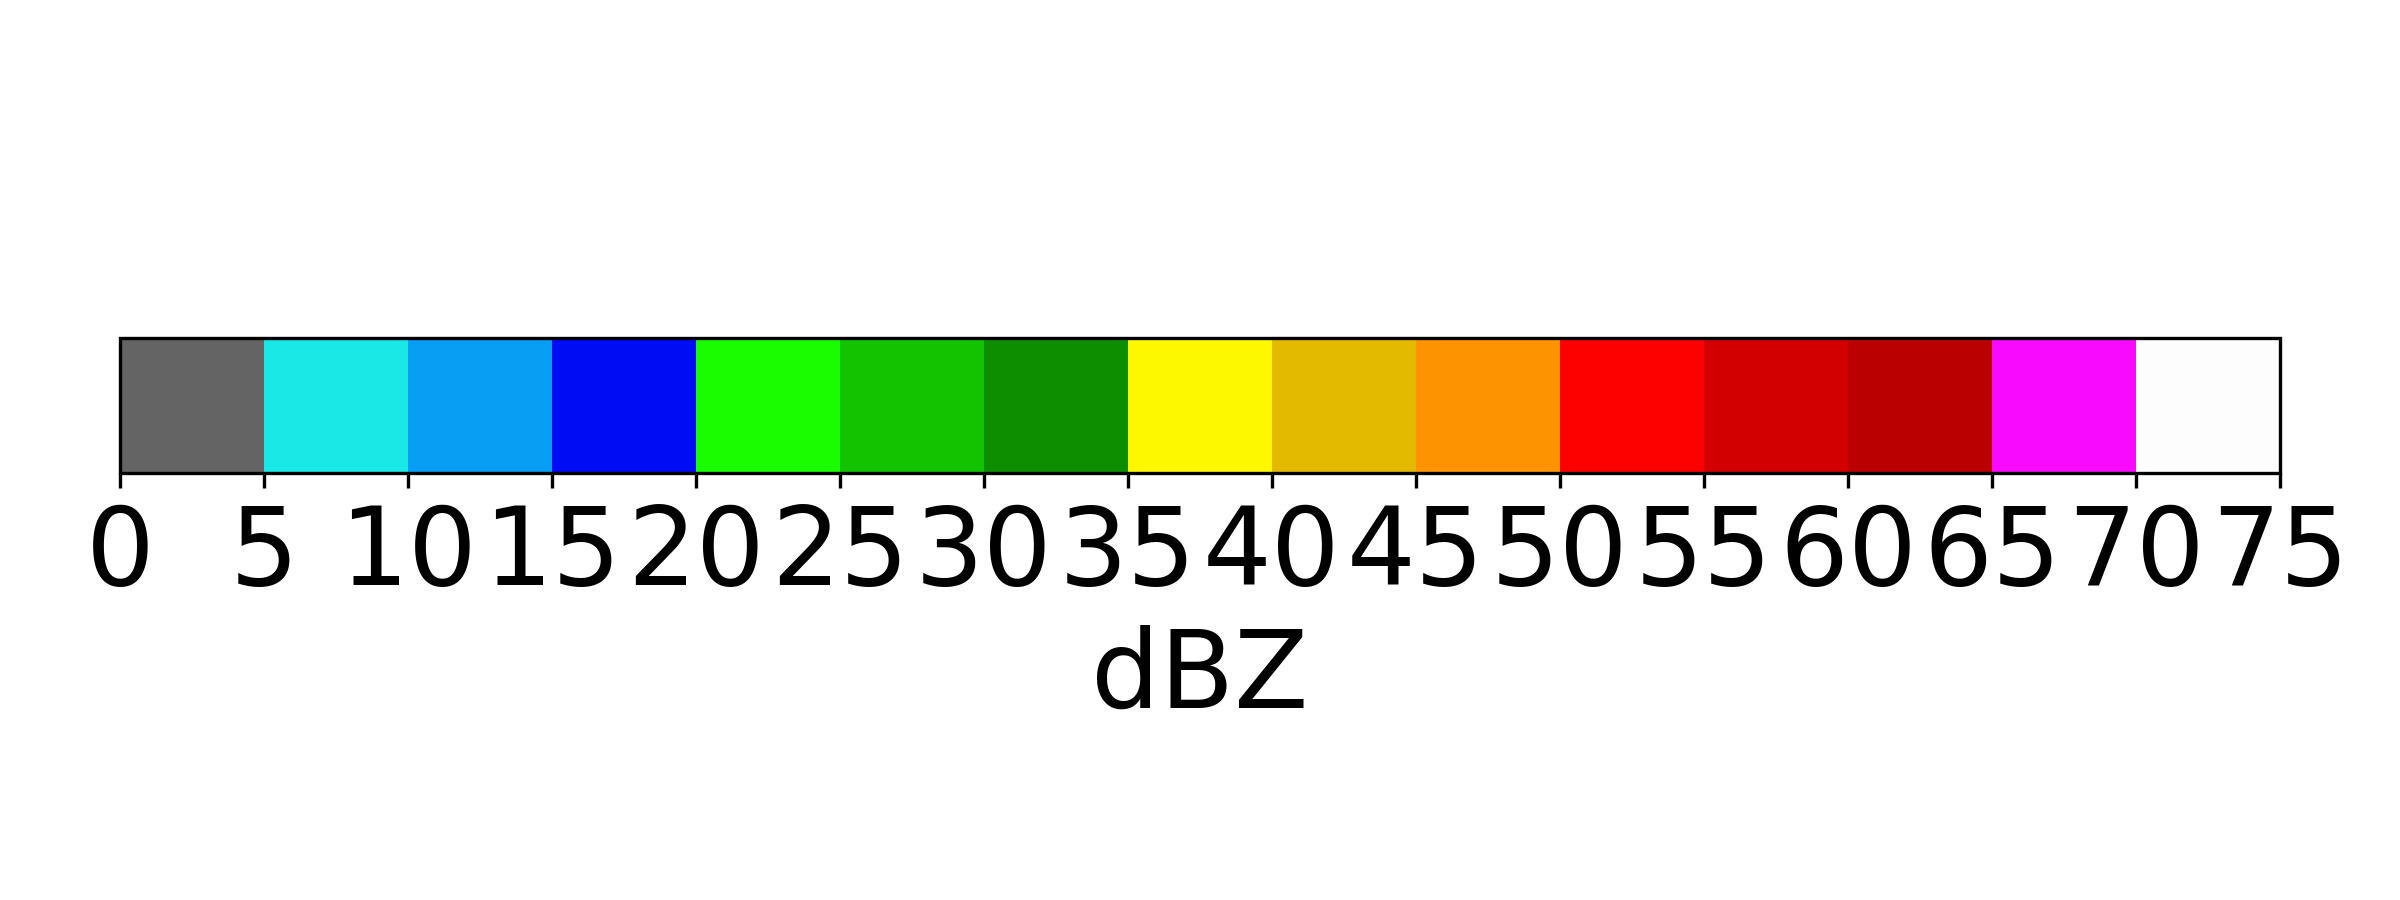
\includegraphics[width=\textwidth]{./thesis_code/plots/dfw_colormap.png}
		\caption{20180607}
		\label{fig:classifying_datadiscovery_ex2}
	\end{subfigure}
	\begin{subfigure}[b]{0.45\textwidth}
		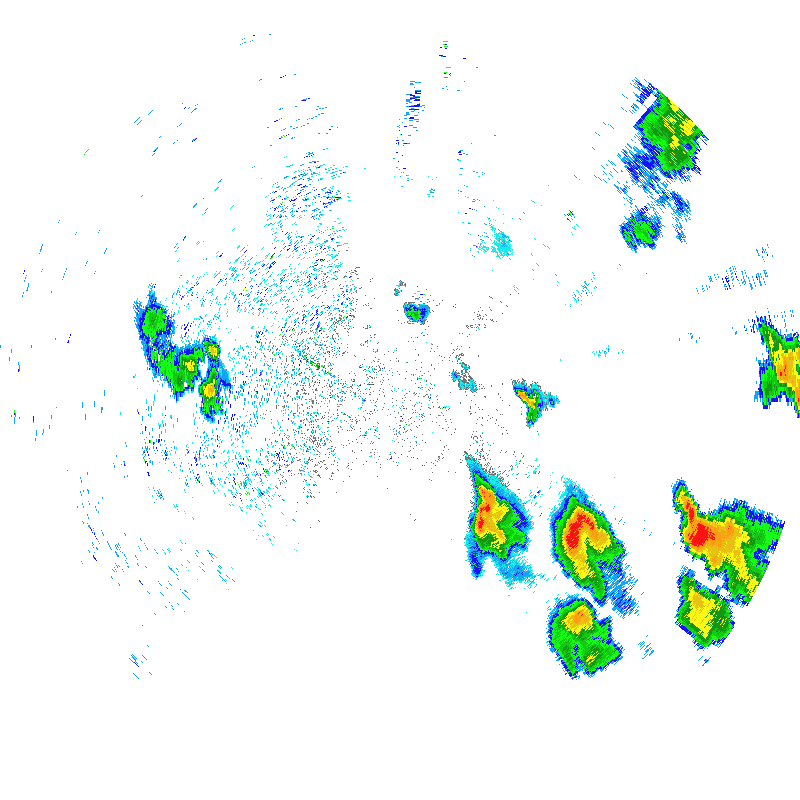
\includegraphics[width=\textwidth]{./thesis_code/plots/midlothian-tx-20180605-104436-ref.png}
		\caption{20180605}
		\label{fig:classifying_datadiscovery_ex3}
	\end{subfigure}
	\begin{subfigure}[b]{0.45\textwidth}
		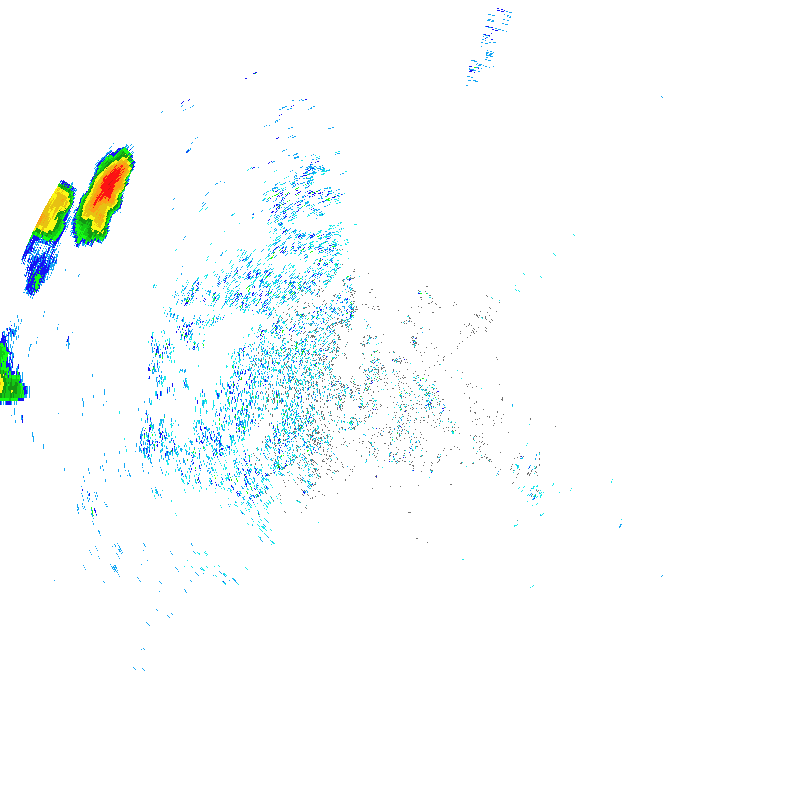
\includegraphics[width=\textwidth]{./thesis_code/plots/midlothian-tx-20180624-063650-ref.png}
		\caption{20180624}
		\label{fig:classifying_datadiscovery_ex4}
	\end{subfigure}
	\caption{Example data that was discovered by model and labeled as convective precipitation. These scans were selected randomly from a large dataset from the month of June 2018, at the XMDL radar. Expert human curation is needed, though these four samples certainly represent the expected precipitation regime.}
	\label{fig:classifying_datadiscovery}
\end{figure}

\begin{figure}[ht]
	\centering
	\begin{subfigure}[b]{0.45\textwidth}
		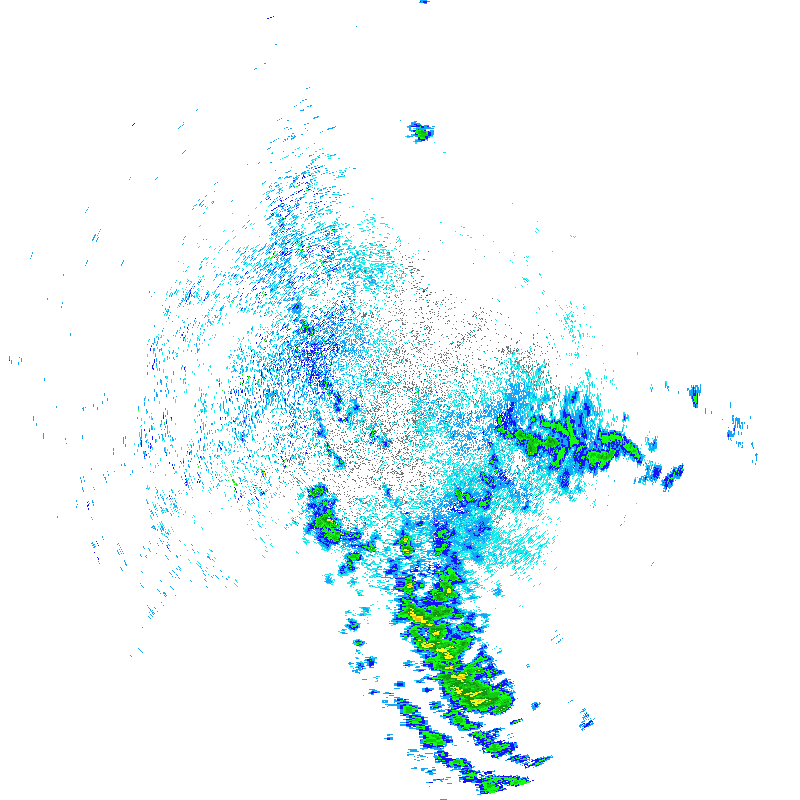
\includegraphics[width=\textwidth]{./thesis_code/plots/midlothian-tx-20180903-063419-ref.png}
		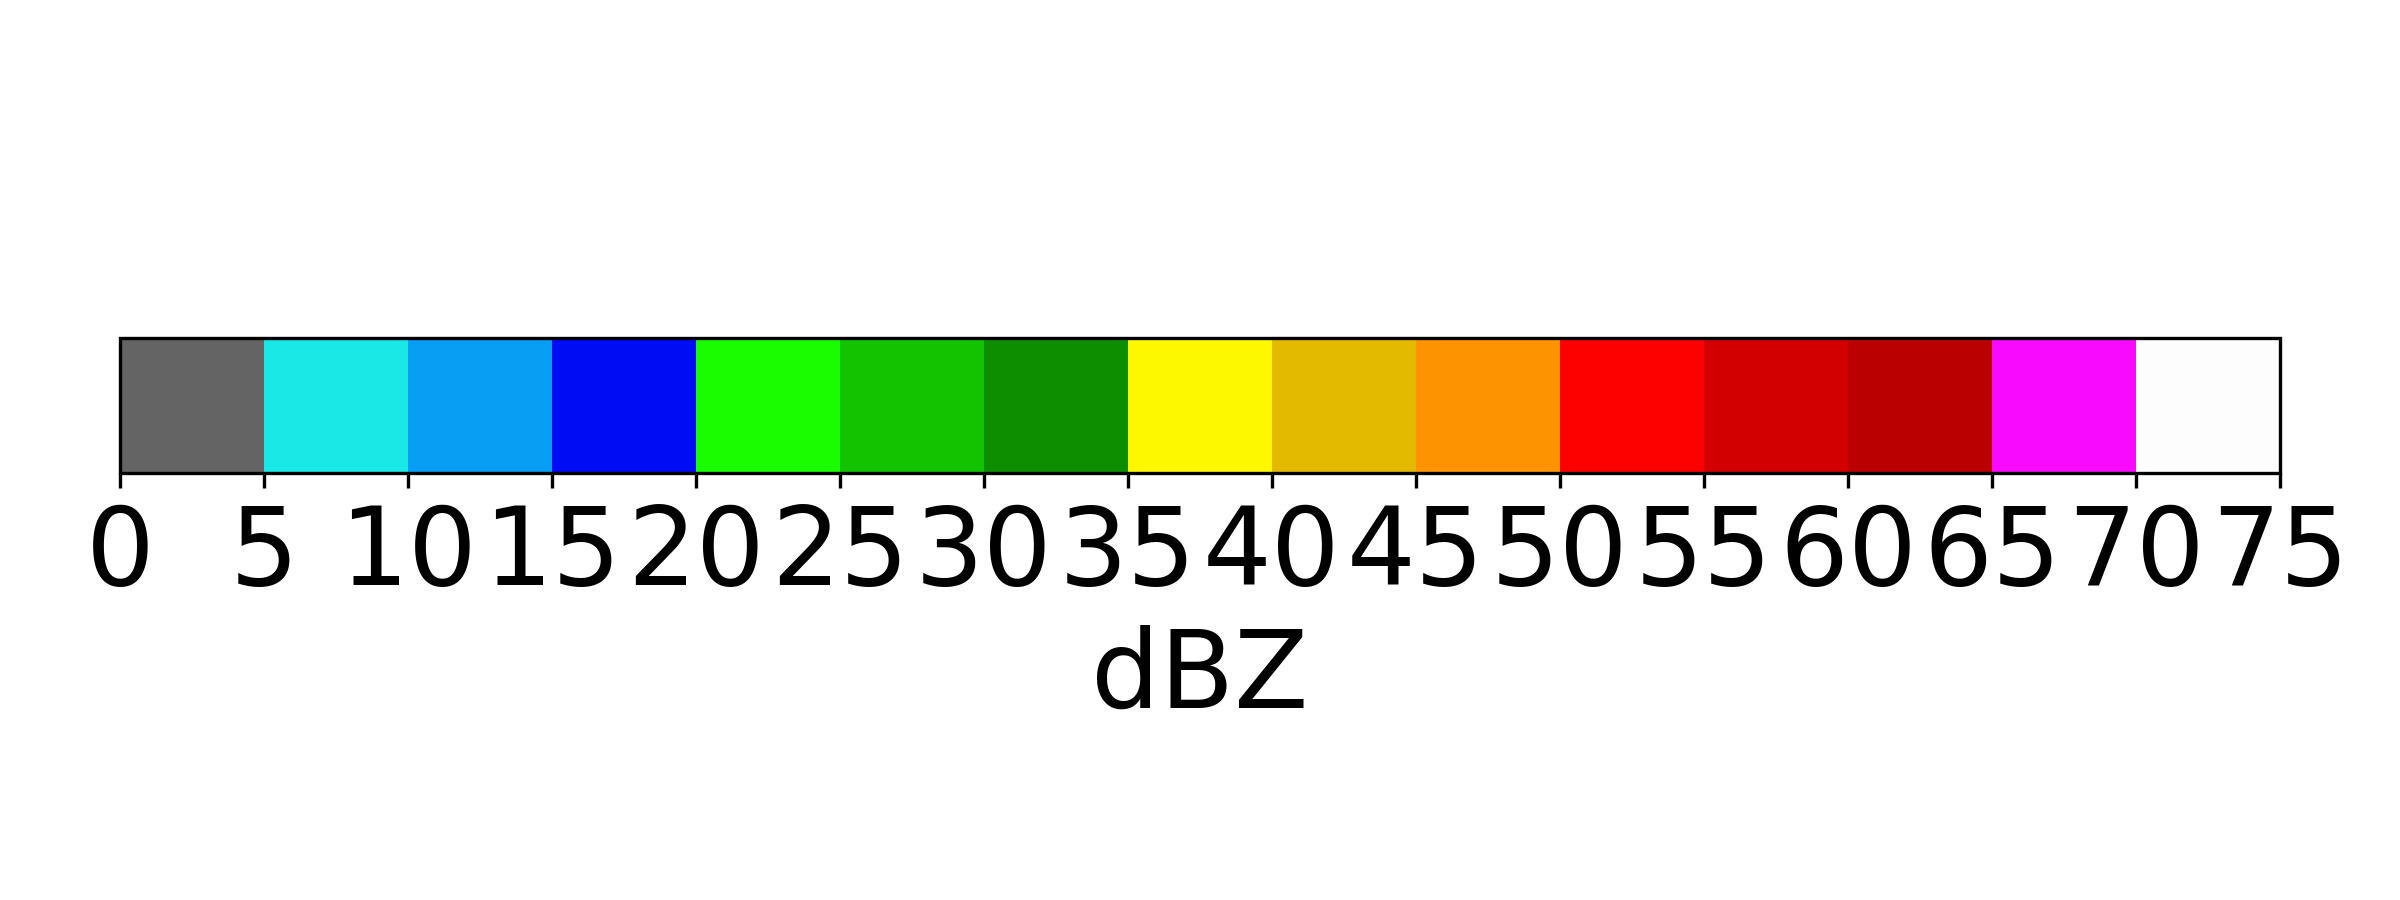
\includegraphics[width=\textwidth]{./thesis_code/plots/dfw_colormap.png}
		\caption{20180903 - Predicted Convective}
		\label{fig:classifying_datadiscovery_ex5}
	\end{subfigure}
	\begin{subfigure}[b]{0.45\textwidth}
		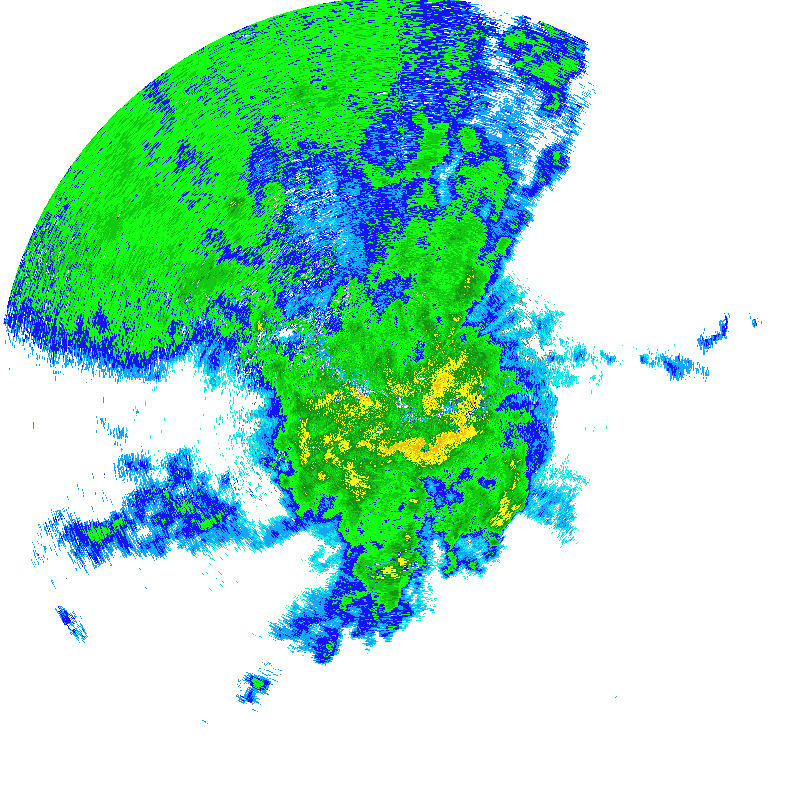
\includegraphics[width=\textwidth]{./thesis_code/plots/midlothian-tx-20180908-173505-ref.png}
		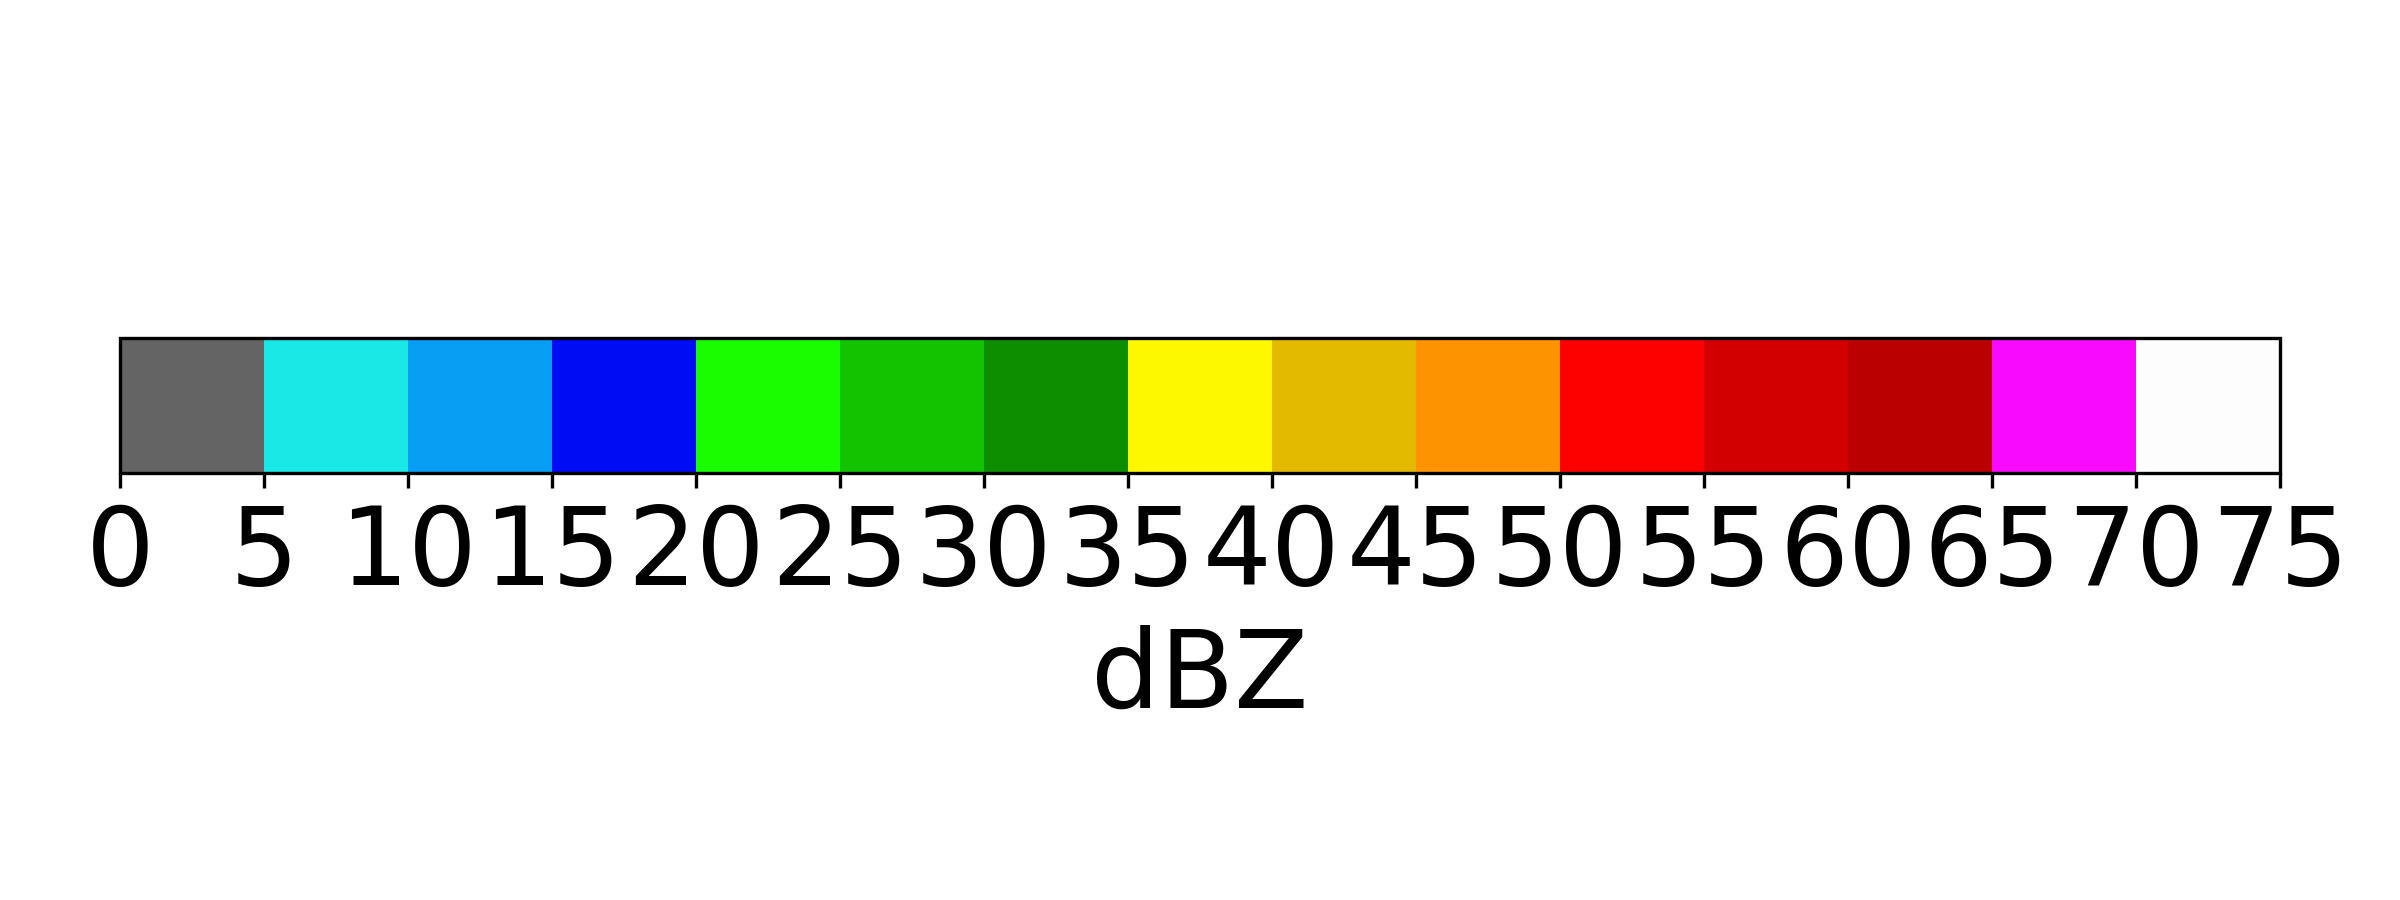
\includegraphics[width=\textwidth]{./thesis_code/plots/dfw_colormap.png}
		\caption{20180908 - Predicted Stratiform}
		\label{fig:classifying_datadiscovery_ex6}
	\end{subfigure}
	\begin{subfigure}[b]{0.45\textwidth}
		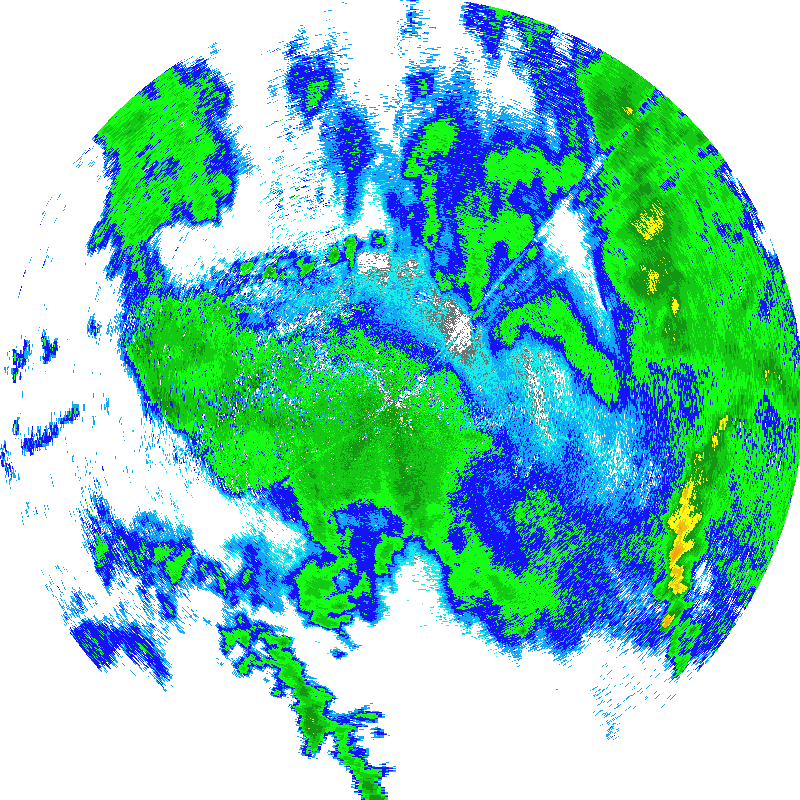
\includegraphics[width=\textwidth]{./thesis_code/plots/midlothian-tx-20180922-105742-ref.png}
		\caption{20180922 - Predicted Stratiform}
		\label{fig:classifying_datadiscovery_ex7}
	\end{subfigure}
	\begin{subfigure}[b]{0.45\textwidth}
		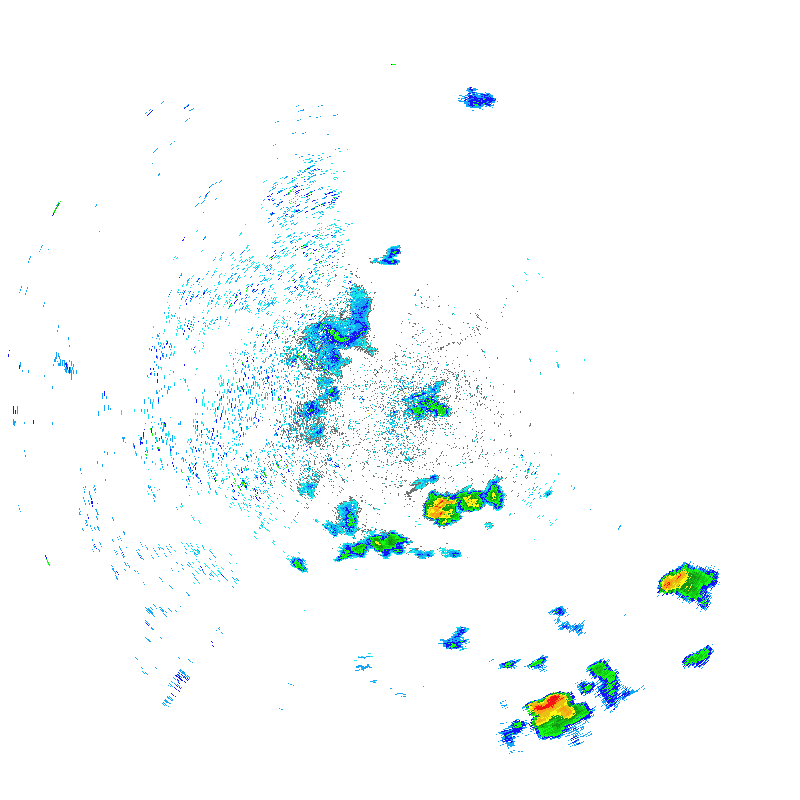
\includegraphics[width=\textwidth]{./thesis_code/plots/midlothian-tx-20180929-202320-ref.png}
		\caption{20180929 - Predicted Stratiform}
		\label{fig:classifying_datadiscovery_ex8}
	\end{subfigure}
	\caption{Example data that was discovered by model. These scans were selected randomly from a large dataset from the month of June 2018, at the XMDL radar. Unlike in Figure \ref{fig:classifying_datadiscovery}, there were more stratiform predictions.}
	\label{fig:classifying_datadiscovery_201809}
\end{figure}

\subsection{CASA - Generated RGB Colormapped Images}
\label{ssec:classifying_casargbdiscovery}

We can generate three-channel pseudo-images where each channel in the image encodes data from different radar variables.
This sort of research has been tested in assisting human visualization and classification before, but it is hypothesized that this could assist a deep learning model in making inferences, especially regarding localized phenomena where radar variable interactions must be considered in order to make correct classifications.
This is an area of proposed research.
\chapter{Discovering the Optimum Model and Increasing Dataset Size}
\label{sec:bestmodel}
% Discuss updates since Prelim, including increasing dataset size and discovery of best model

Various issues arise in the preceding chapters regarding the classification system developed and dataset compiled.
A brief list of such issues includes:

\begin{itemize}
	\item Limited labeled dataset
	\item Restricted generalization ability of the model
	\item Lack of integration of recent developments in image-based machine learning techniques
\end{itemize}

As previously discussed, the initial dataset includes, in total, roughly 1,200 weather radar images.
This dataset was compiled by the author's careful inspection of hundreds of thousands of images and labeled by hand when a particular meteorological phenomena or precipitation regime was present.
The data corpus was constructed of scans from one X-band radar, located in Midlothian, TX, with time coverage between January 2016 to December 2017.
Given that plan-position indicator (PPI) scans are produced at the 1 degree elevation every minute, there are roughly 500,000 scans available each year.
Even with diligent searching and labeling, many potentially valuable radar scans representing phenomena of interest will be missed.

Part of the inspiration for this work, and indeed a major goal, however, was to be able to apply a "less-educated" model to new data, produce what may be referred to as "less-educated guesses" as to class membership on said new data, and allow a human expert the ability to peruse these guesses and correct mistakes made in terms of false positives and false negatives.
This process greatly reduces the time taken to label the many thousands of candidate images and generates an opportunity to increase the dataset size by an order of magnitude.

The second item in the list above goes hand-in-hand with the first item, in that in order to improve the generalization ability of the model, we must be able to train the model using many more representations of classes of interest.
To do this, we must include more data.

\begin{figure}[h]
	\centering
	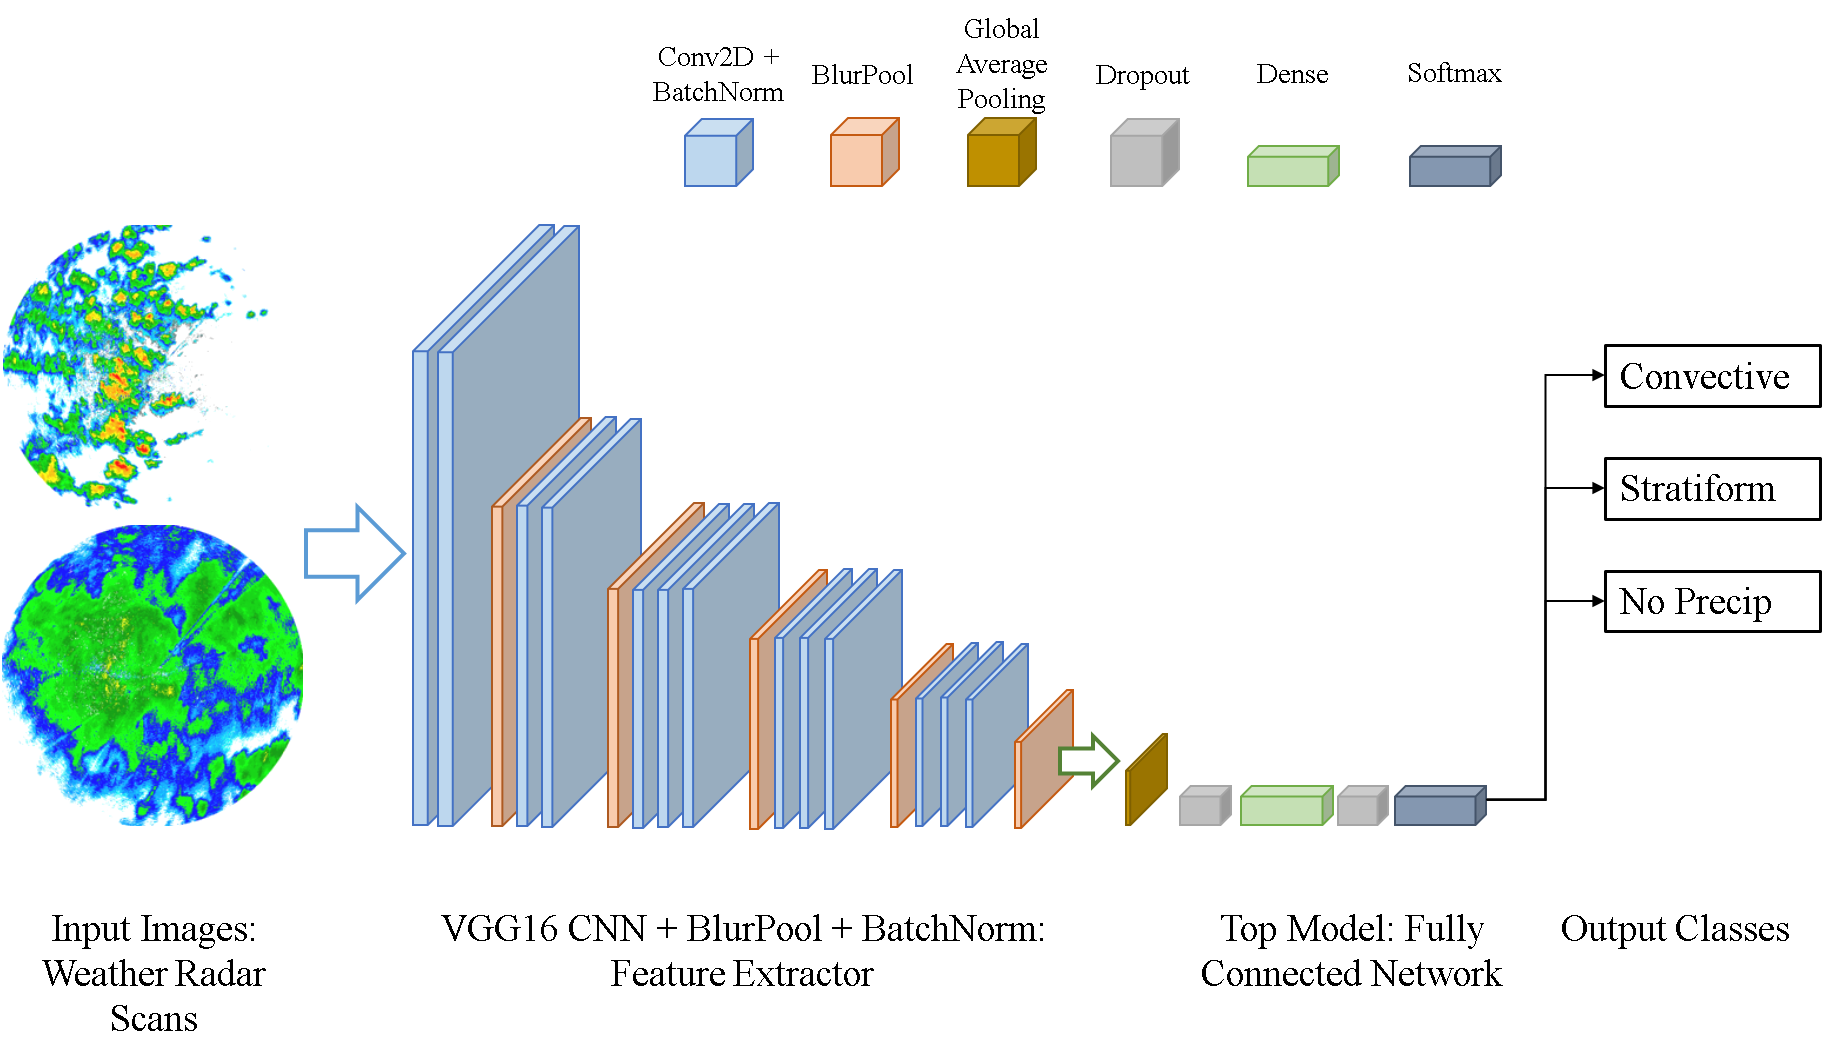
\includegraphics[width=\textwidth]{./thesis_code/plots/DL-workflow.png}
	\caption{Complete end-to-end deep learning architecture devised in this chapter. Note that convolution layers now include batch normalization, while downsampling layers are formed by the new BlurPool layer. These two are tuneable parameters in this architecture, and we tested many configurations to find the best set of parameters and hyperparameters.}
	\label{fig:end-to-end}
\end{figure}

The third item can be used to assist the second item as well. Computer vision, transfer learning, and machine learning in general are currently some of the most active areas of research in science as a whole.
The tools that are being developed, and indeed, that have been developed, can find application in almost every field, and each field in turn can offer insight into improving the tools themselves.
It is essentially impossible for any one researcher or team of researchers to stay abreast of every relevant development related to their field.
However, leveraging insights made from recent discoveries remains useful, important, and essential for any effort in this field.

To that end, we propose a set of experiments to determine the optimal model to use for our transfer learning procedure by incorporating recent discoveries from the field into our deep learning model architecture, and testing each variation on a consistent dataset to determine the best architecture.
The following sections in this chapter detail the efforts made to increase the dataset size, descriptions of the additional model layers, and present the results of the set of experiments that yields the optimum model, given these alterations and improvements.
We illustrate that the optimum model from the tested configurations is shown in the end-to-end architecture diagram in Figure \ref{fig:end-to-end}.

\section{Increased Dataset Size}
\label{sec:bestmodel_dataset}

\section{BlurPool}
\label{sec:bestmodel_blurpool}

A dataset must include many representations of the desired phenomena of interest in order to allow better generalization on test sets.
In the specific case of weather radar data, however, it is likely to see scans that are highly visually similar to one another when successive scans are recorded in one minute intervals, as the images in this study are produced.
This high level of inter-image intercorrelation may lead to instances of overfitting, if the training dataset is not large enough to present many uncorrelated events, as well as many scans for each event.
Storms and weather precipitation events will tend to move slowly across the high-resolution, large geographic sampling area present in each scan, leading to the same or similar echoes occurring in tens of successive scans as represented in Figure \ref{fig:bestmodel_translation}.
It is thus desirable to not only encourage generalizability to unseen data in a particular classifier, but in this case, to also be resilient to image object translation.

\begin{figure}[h]
	\centering
	\begin{subfigure}[b]{0.3\textwidth}
		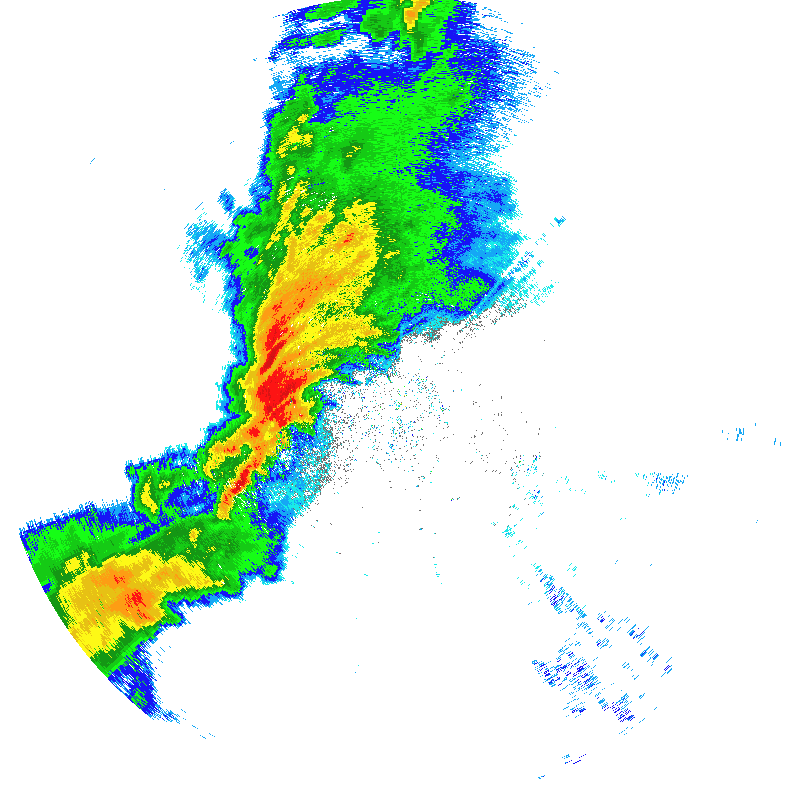
\includegraphics[width=\textwidth]{./thesis_code/plots/midlothian.tx-20180421-235038-ref.png}
		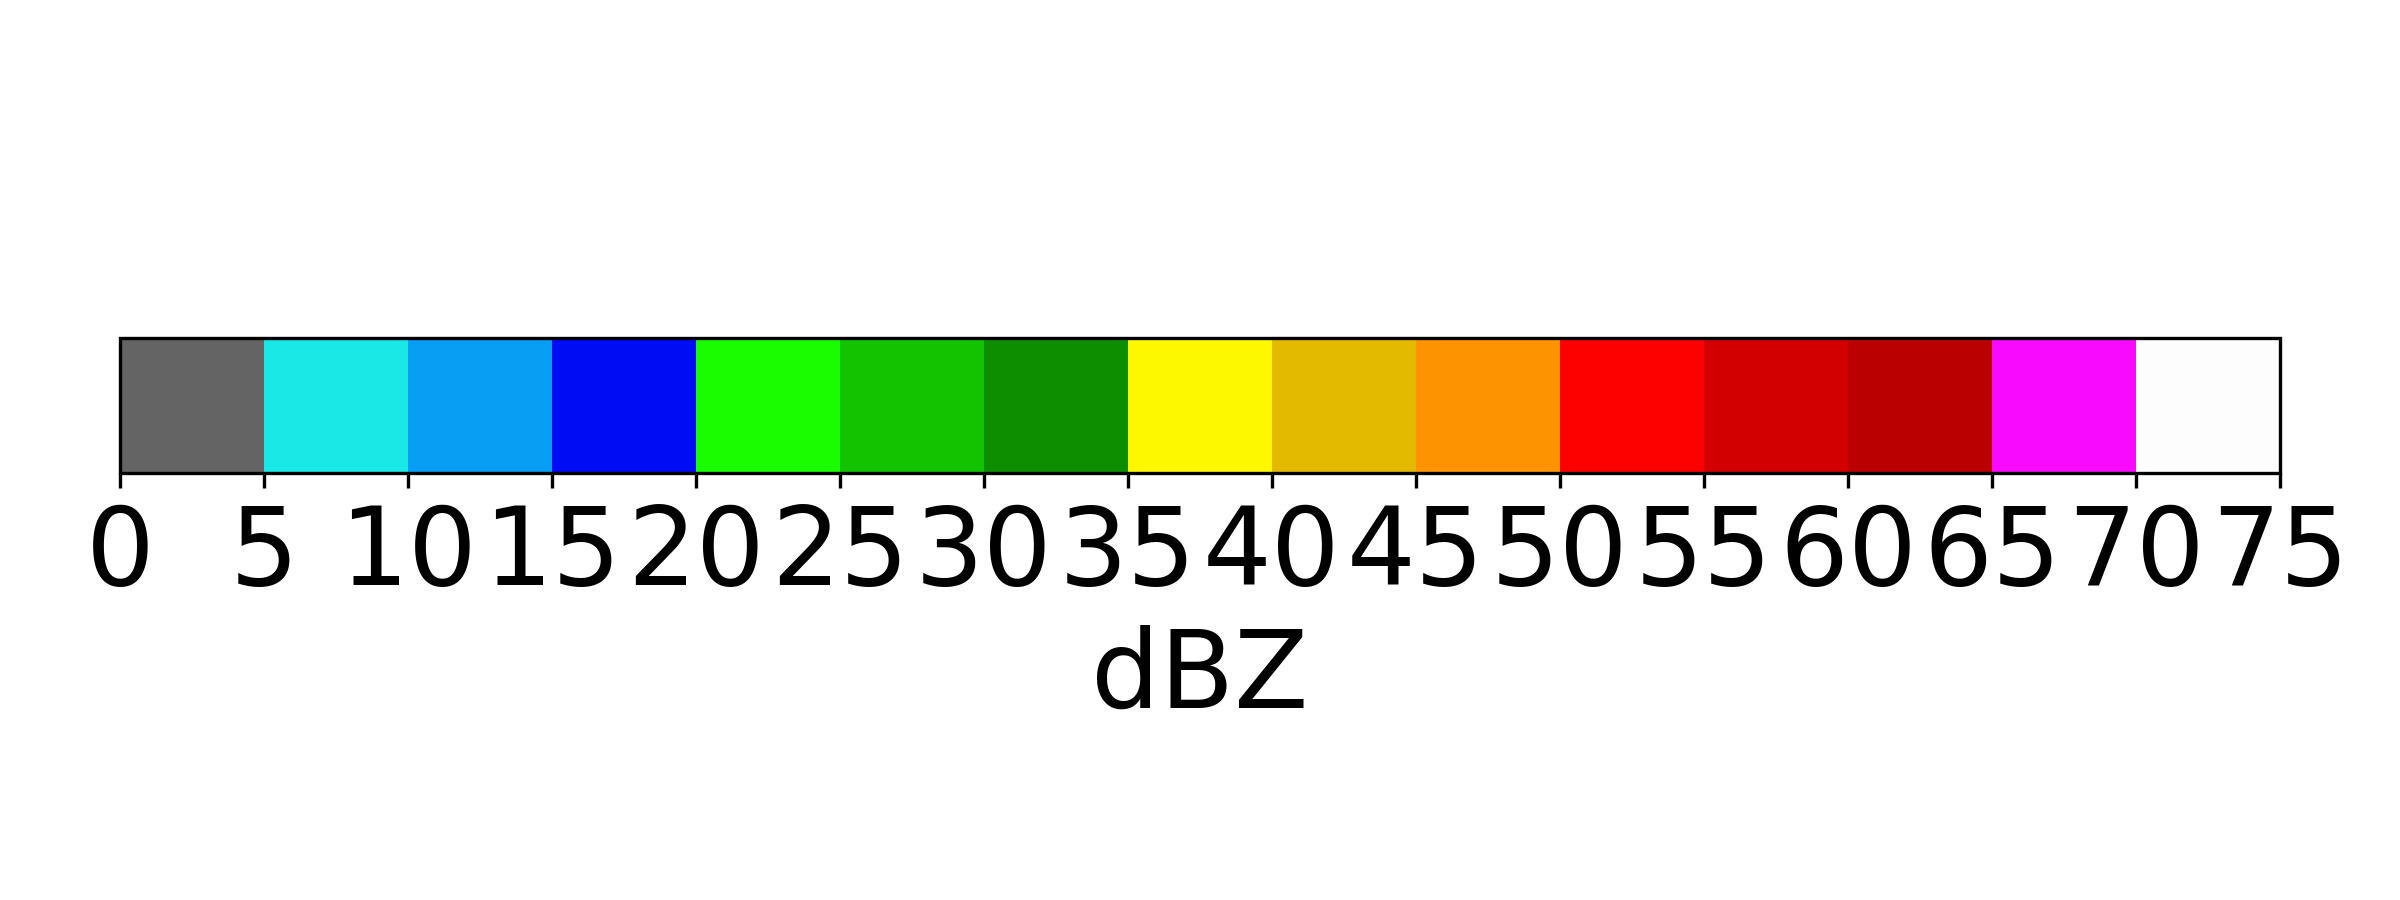
\includegraphics[width=\textwidth]{./thesis_code/plots/dfw_colormap.png}
		\caption{2018-04-21 23:50:38 UTC}
		\label{fig:bestmodel_translation1}
	\end{subfigure}
	\begin{subfigure}[b]{0.3\textwidth}
		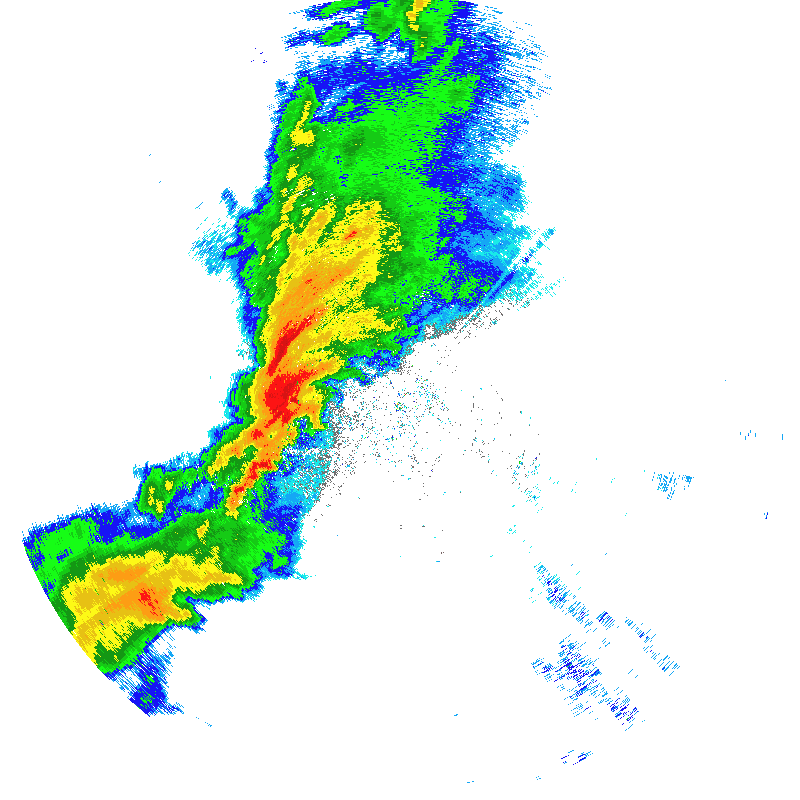
\includegraphics[width=\textwidth]{./thesis_code/plots/midlothian.tx-20180421-235141-ref.png}
		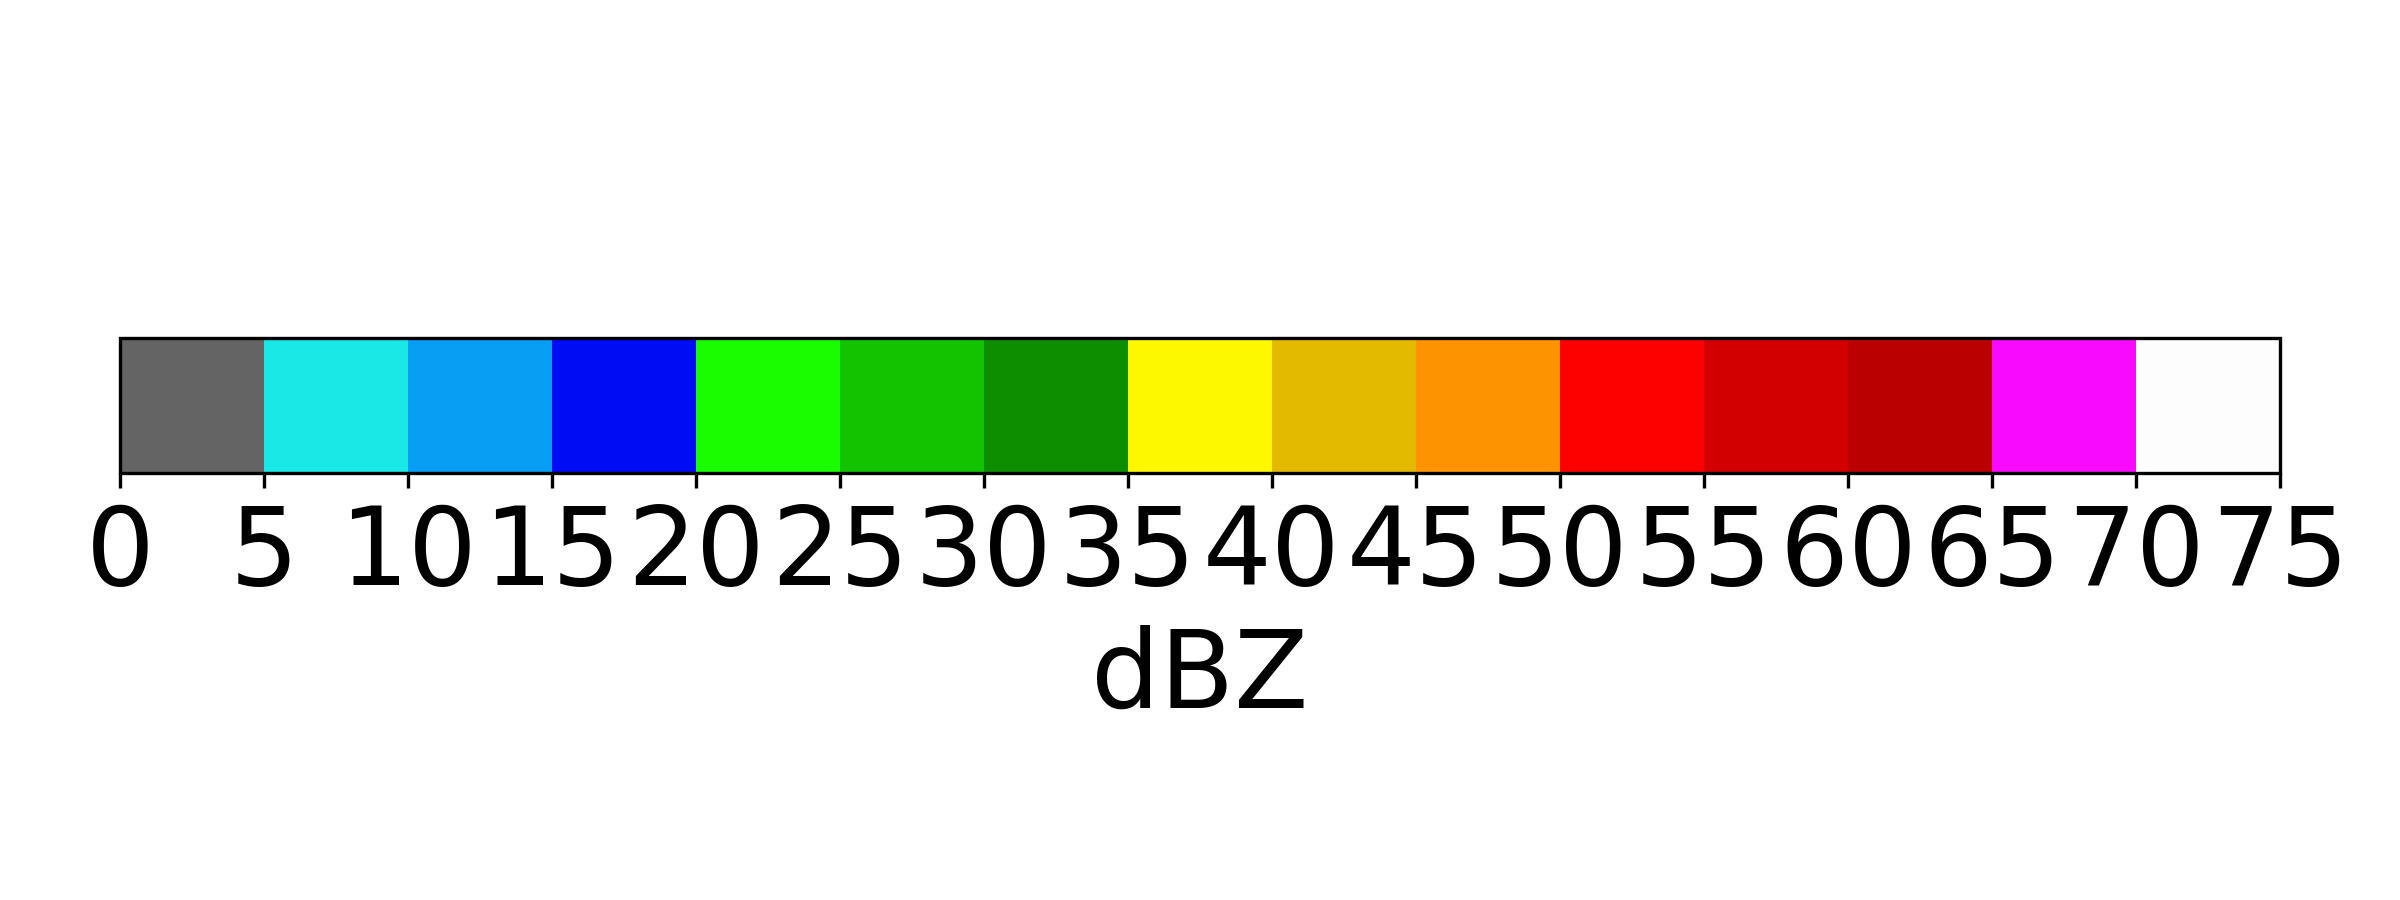
\includegraphics[width=\textwidth]{./thesis_code/plots/dfw_colormap.png}
		\caption{2018-04-21 23:51:41 UTC}
		\label{fig:bestmodel_translation2}
	\end{subfigure}
	\begin{subfigure}[b]{0.3\textwidth}
		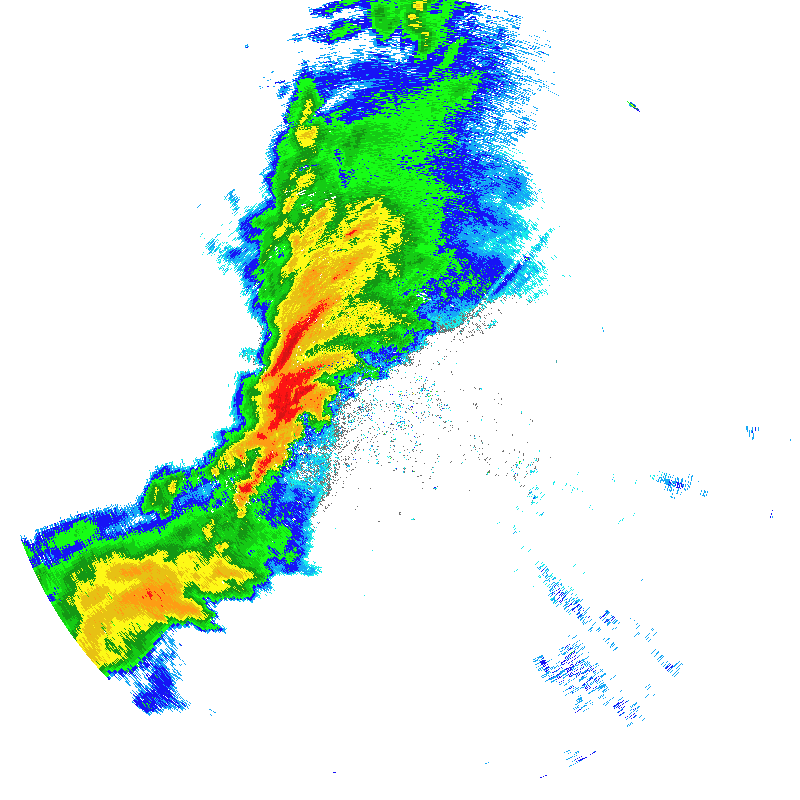
\includegraphics[width=\textwidth]{./thesis_code/plots/midlothian.tx-20180421-235238-ref.png}
		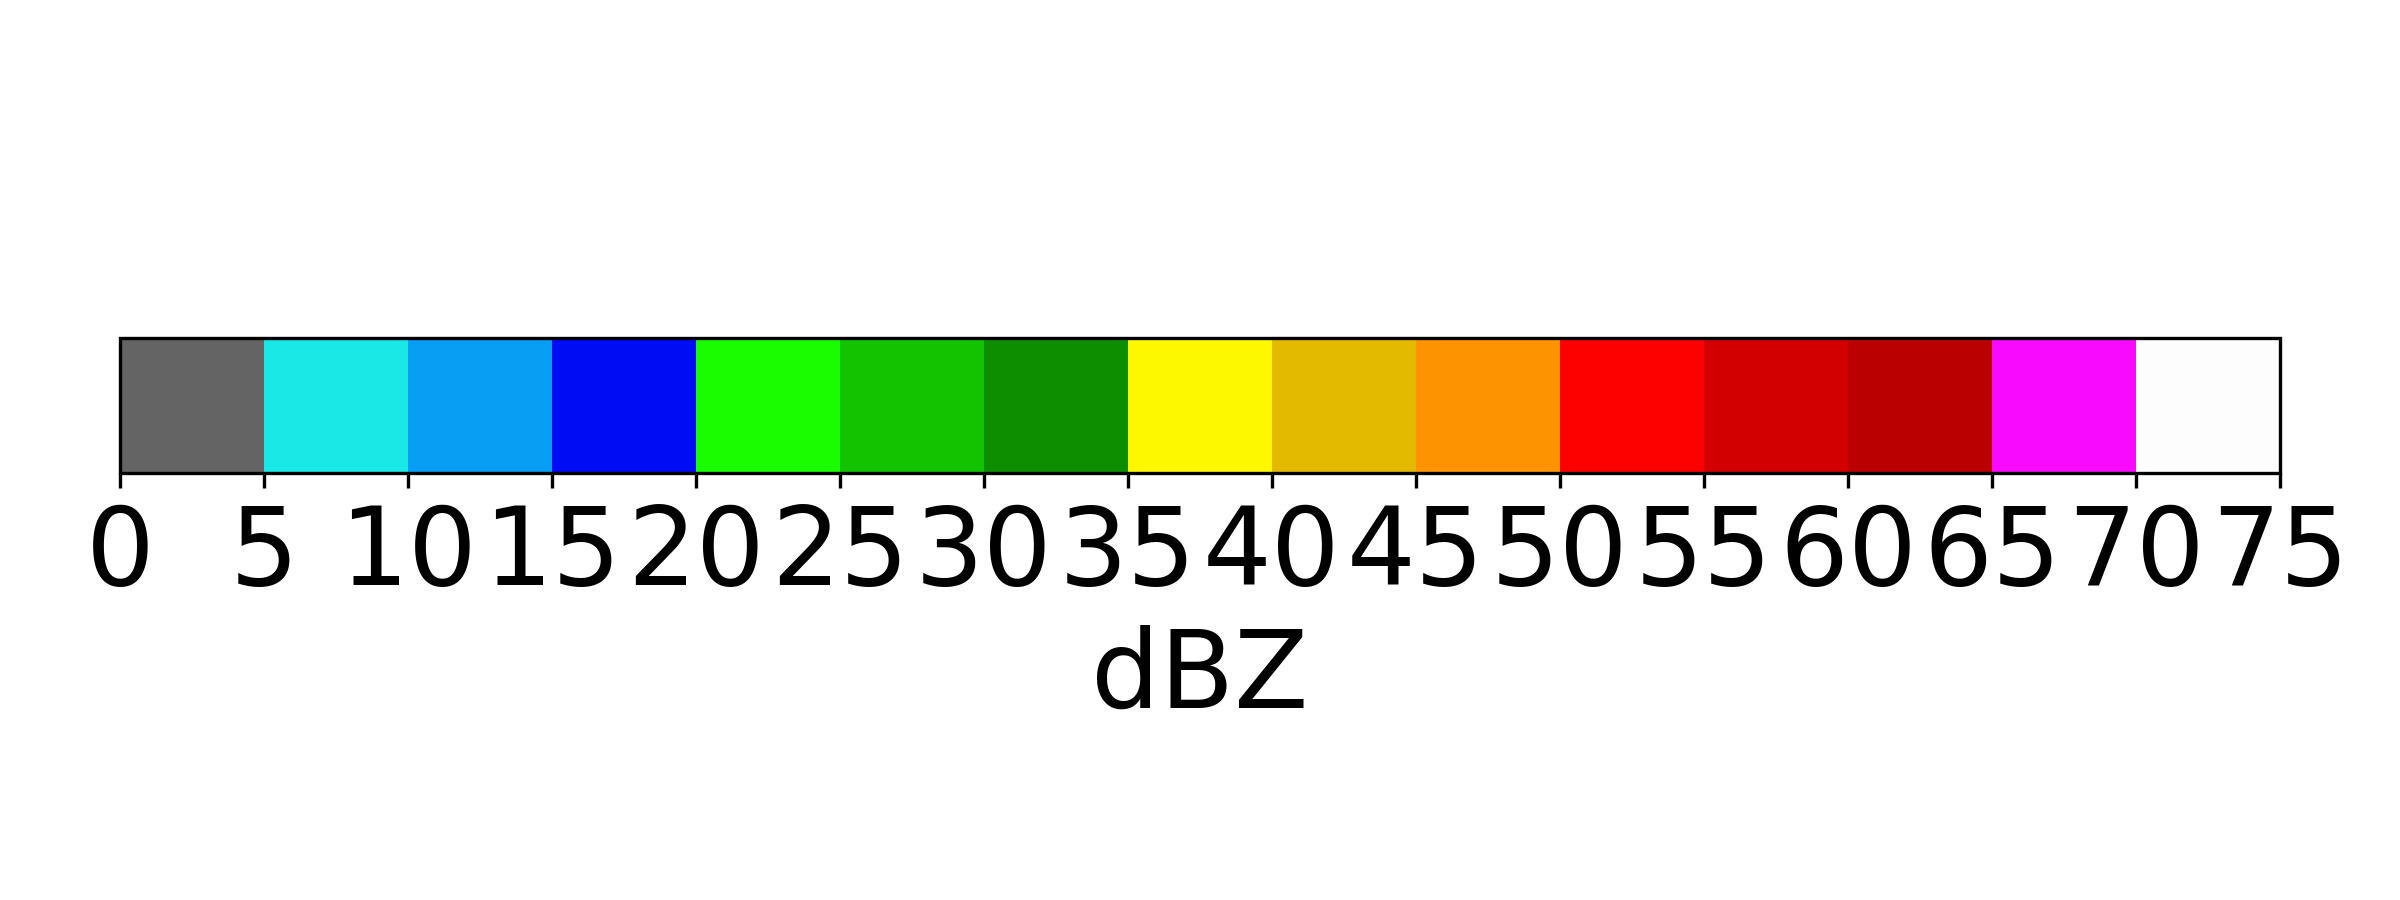
\includegraphics[width=\textwidth]{./thesis_code/plots/dfw_colormap.png}
		\caption{2018-04-21 23:52:38 UTC}
		\label{fig:bestmodel_translation3}
	\end{subfigure}
	\\
	\begin{subfigure}[b]{0.3\textwidth}
		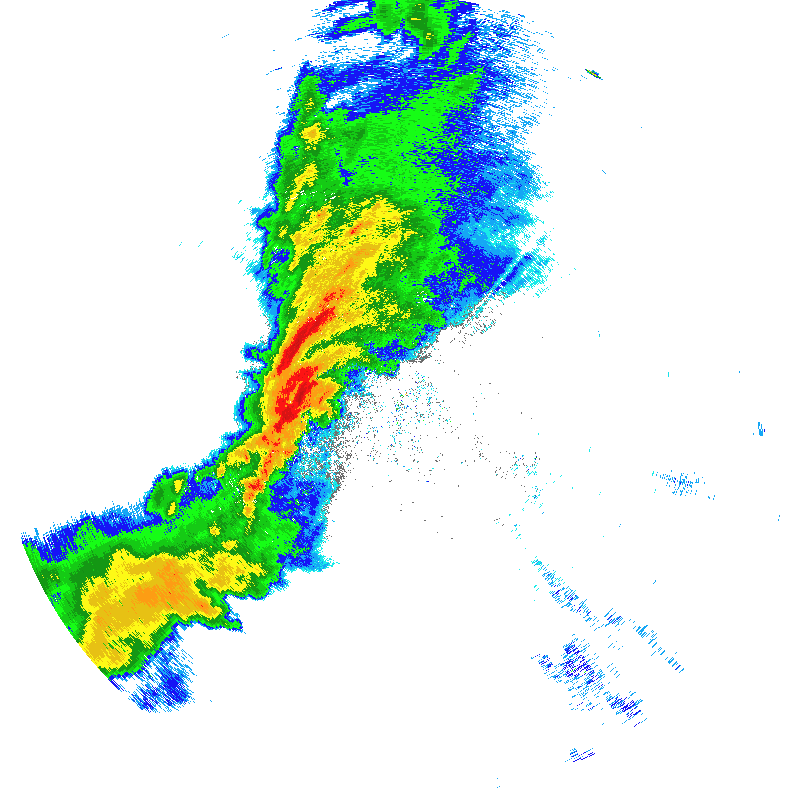
\includegraphics[width=\textwidth]{./thesis_code/plots/midlothian.tx-20180421-235338-ref.png}
		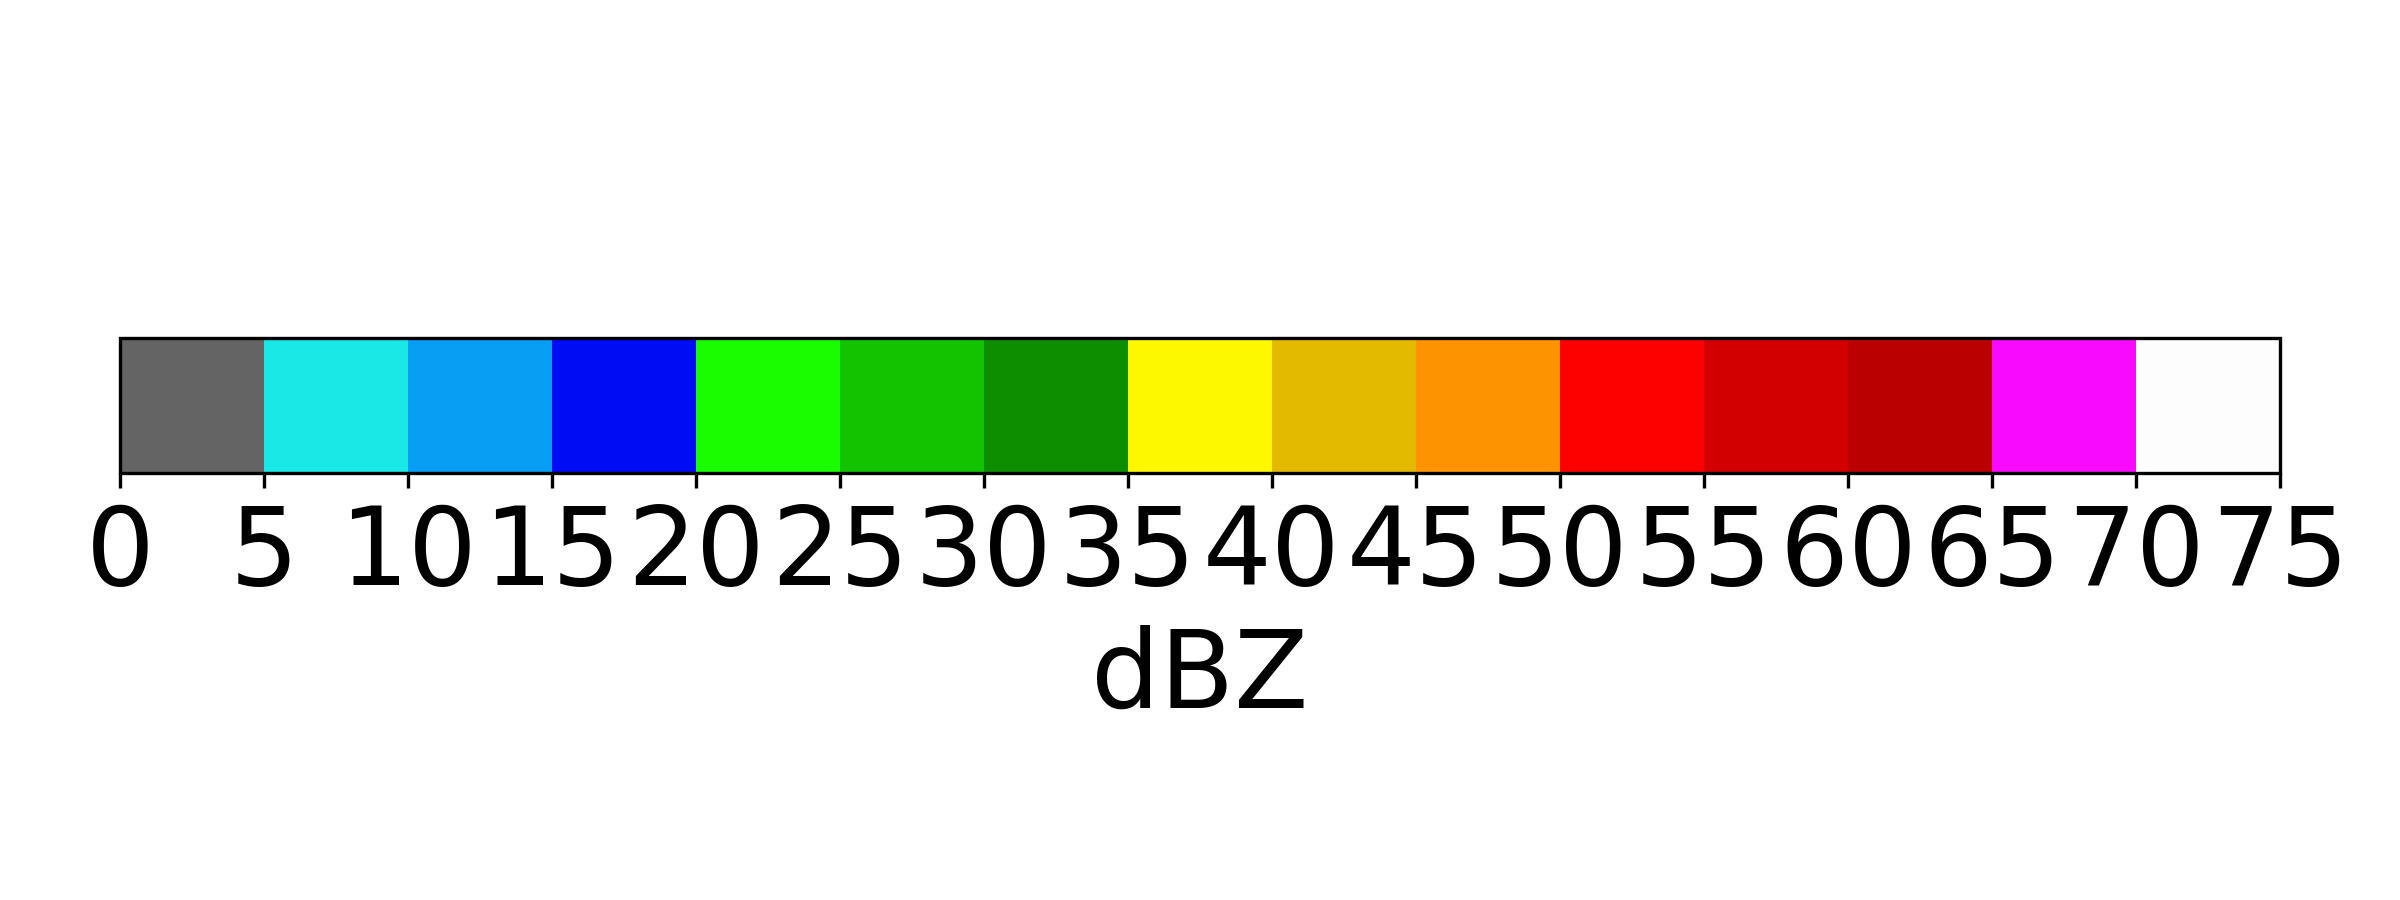
\includegraphics[width=\textwidth]{./thesis_code/plots/dfw_colormap.png}
		\caption{2018-04-21 23:53:38 UTC}
		\label{fig:bestmodel_translation4}
	\end{subfigure}
	\begin{subfigure}[b]{0.3\textwidth}
		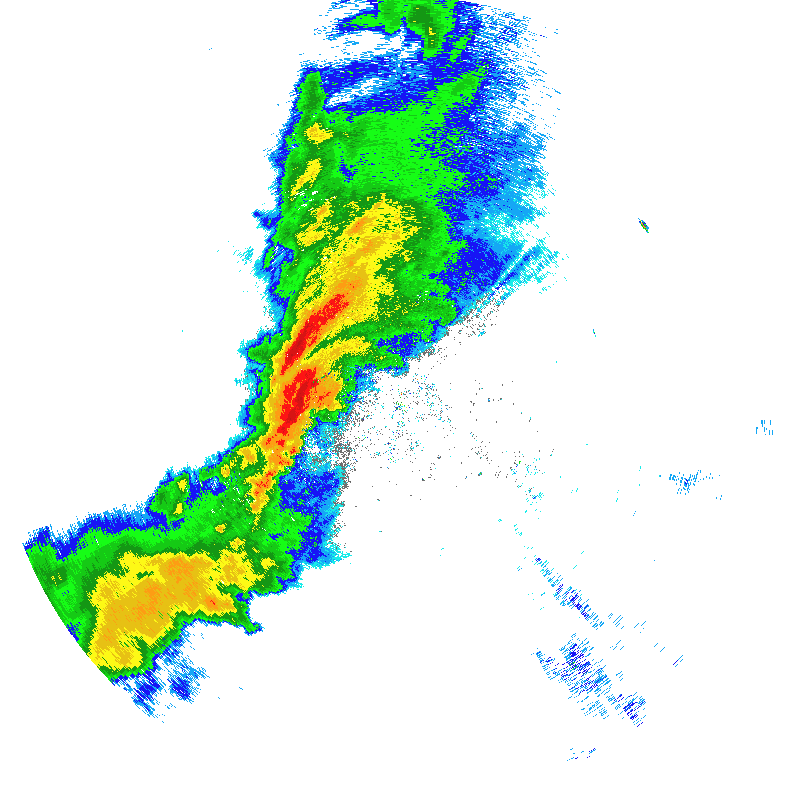
\includegraphics[width=\textwidth]{./thesis_code/plots/midlothian.tx-20180421-235438-ref.png}
		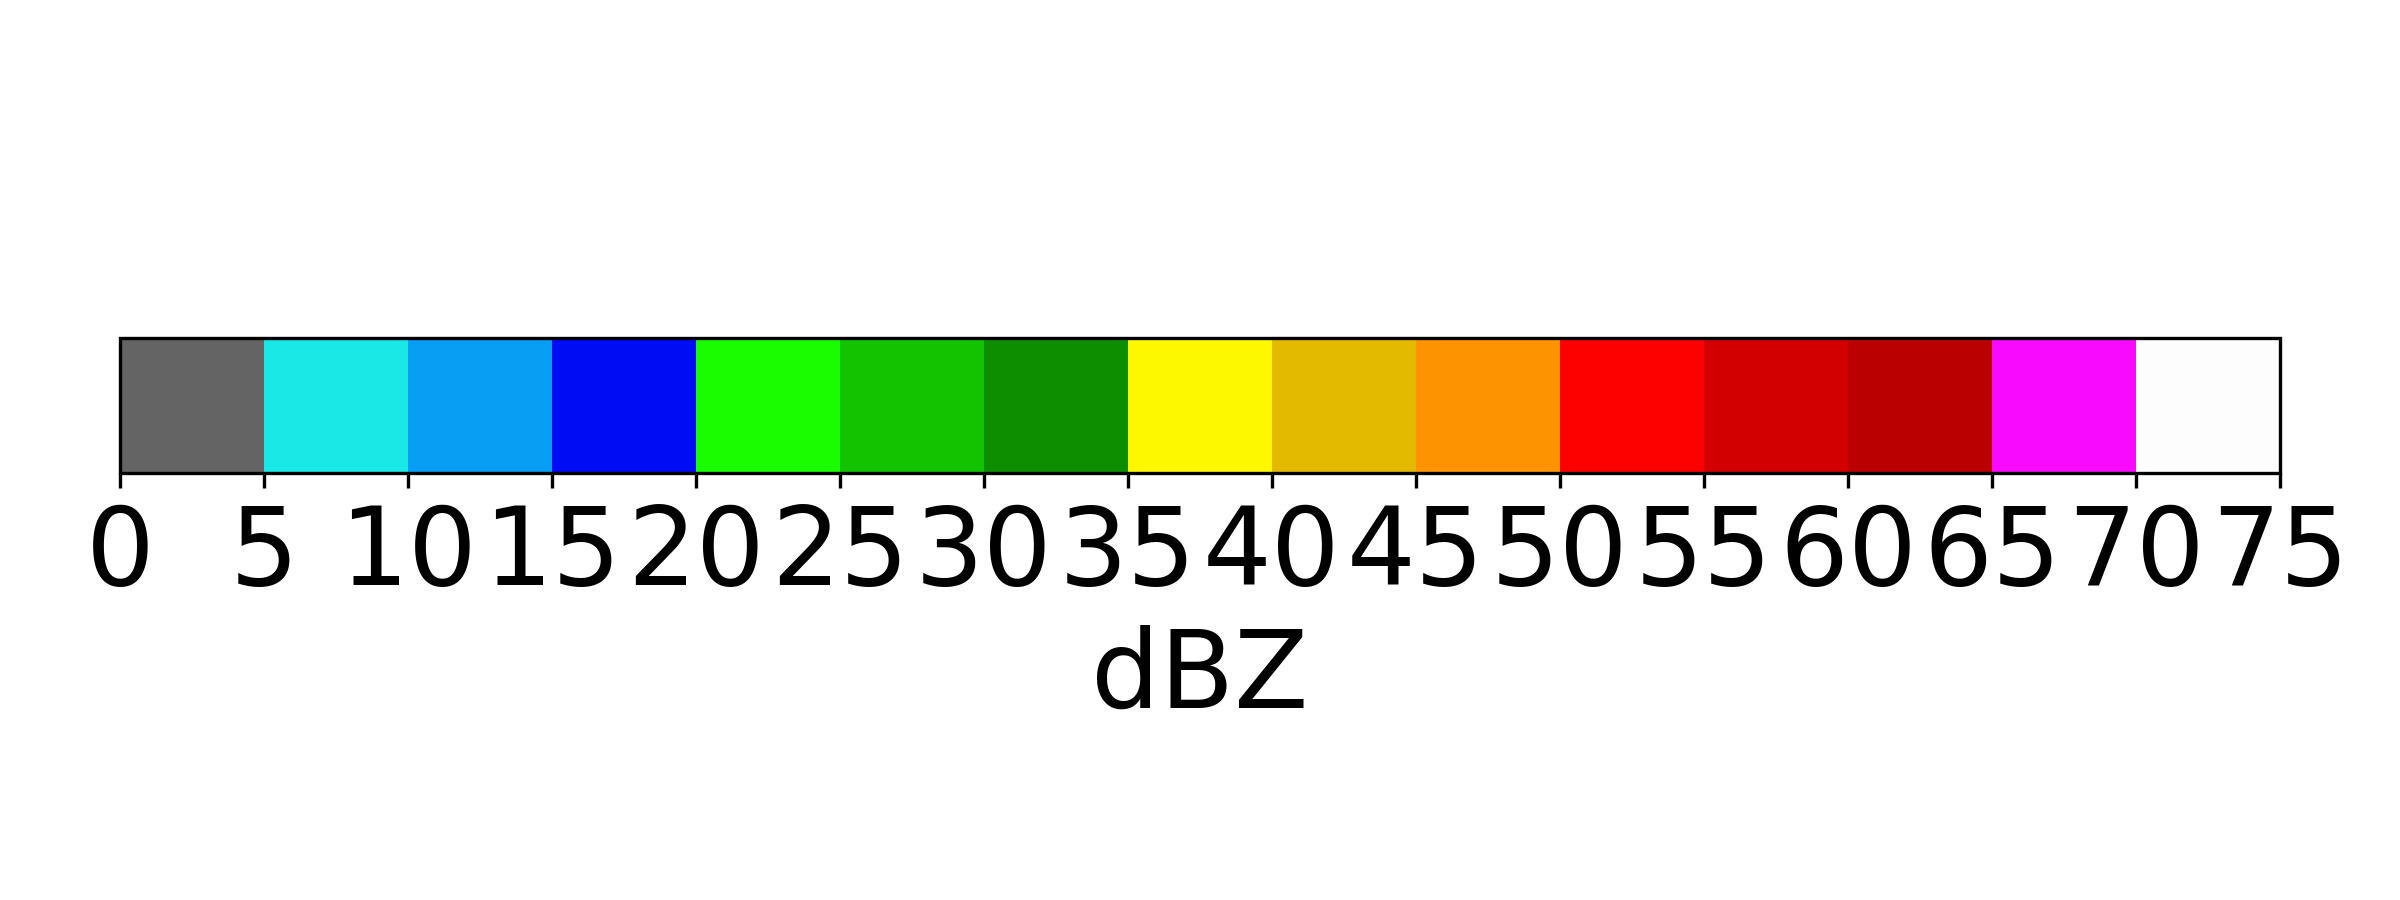
\includegraphics[width=\textwidth]{./thesis_code/plots/dfw_colormap.png}
		\caption{2018-04-21 23:54:38 UTC}
		\label{fig:bestmodel_translation5}
	\end{subfigure}
	\begin{subfigure}[b]{0.3\textwidth}
		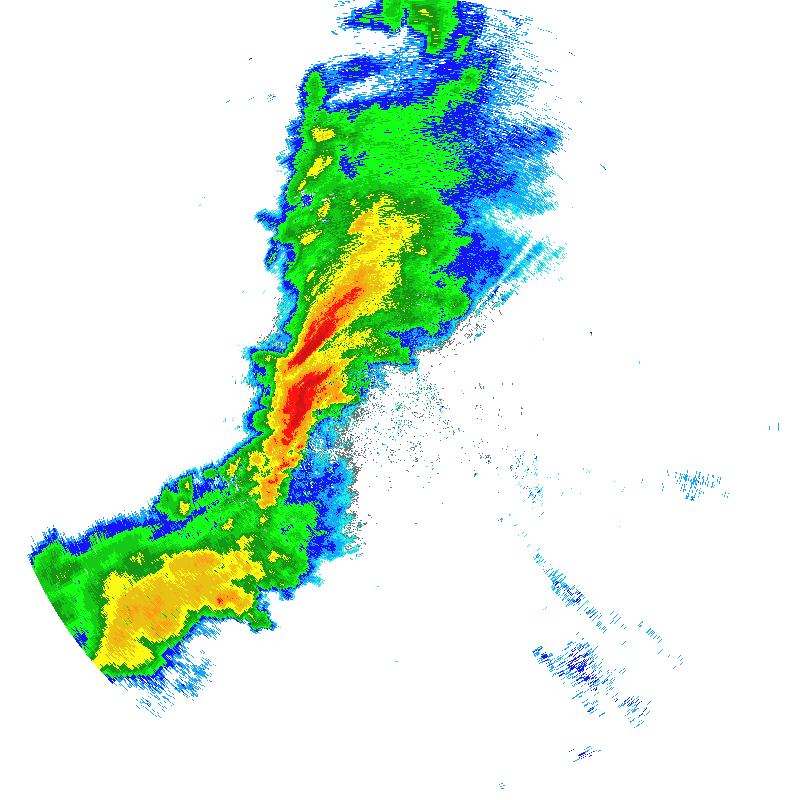
\includegraphics[width=\textwidth]{./thesis_code/plots/midlothian.tx-20180421-235538-ref.png}
		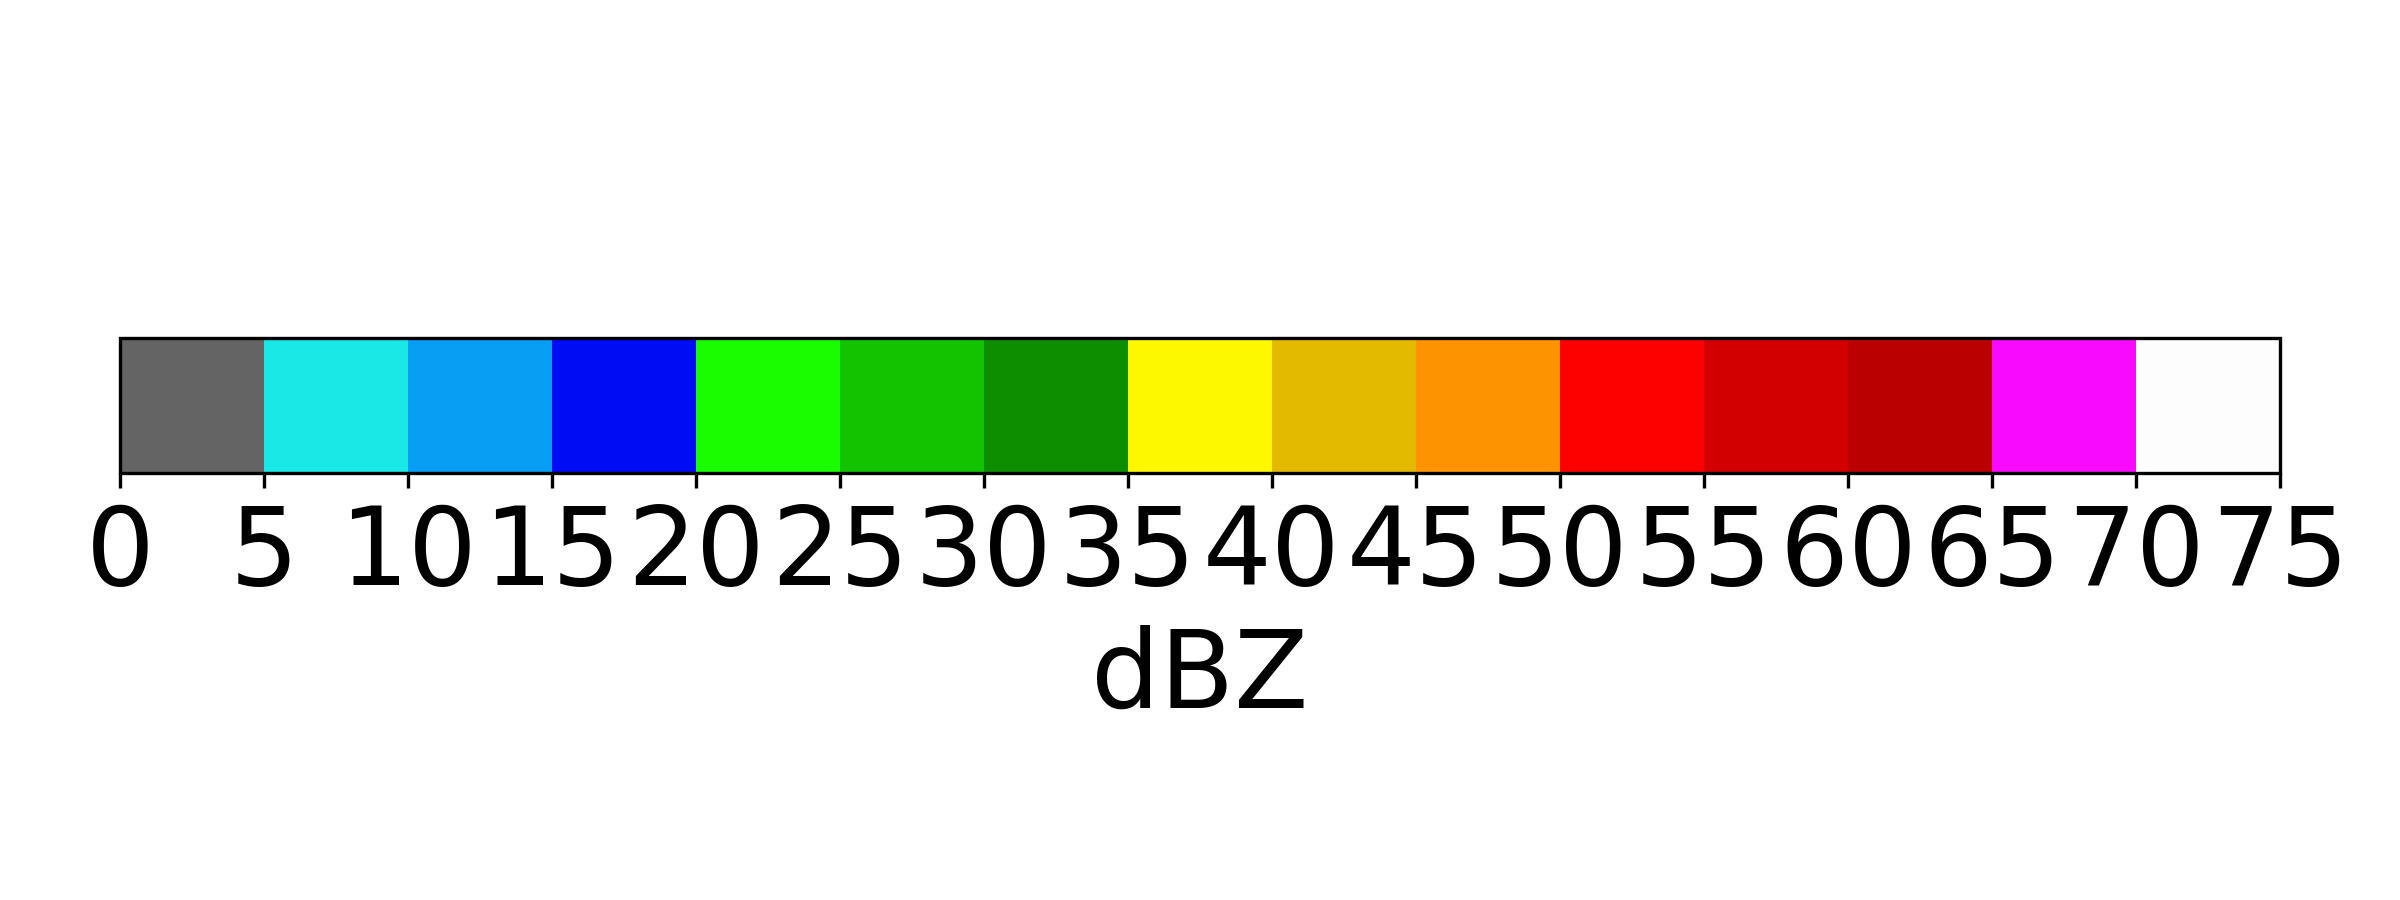
\includegraphics[width=\textwidth]{./thesis_code/plots/dfw_colormap.png}
		\caption{2018-04-21 23:55:38 UTC}
		\label{fig:bestmodel_translation6}
	\end{subfigure}
	\caption{A particular precipitation event as observed in successive scans. Note the similarity between successive scans. In an ideal classifier, all would be classified as "Convective."}
	\label{fig:bestmodel_translation}
\end{figure}

Convolutional neural networks like VGG16 are designed to be resilient to this type of translation, but a recent paper \cite{zhang2019making} illustrated that by replacing the downsampling layer which follows a convolution block, we can gain both accuracy and consistency of prediction.
This layer is called BlurPool, as it is a pooling layer that utilizes a Gaussian blur filter kernel to first low-pass filter the image feature representations following a particular convolution block, before applying the downsampling mechanism.

An important step in any deep learning classifier is the downsampling layer, which takes as input a wider, shallower set of image representations, and reduces the width while increasing the depth.
Width in this context refers to what can be thought of as the number of pixels in the image or image representation, and depth, the number of channels or activations.
We wish to take a high-dimensional input (image), and produce a low dimensional set of predictions (classes).
Thus, these downsampling layers are of critical importance to the deep learning process.

The authors of this paper argue that the current set of most commonly used downsampling layers, however, is not as resilient to translation in input image objects as would be desirable.
They draw inspiration from signal processing, whereby a signal must be low-pass filtered prior to down-sampling, to mitigate issues arising from potential high frequency energy aliasing into lower frequencies.
The current most often used downsampling layers in deep learning models, like max pooling or average pooling, essentially allow this sort of aliasing.
With a Gaussian filter kernel applied to activation layers prior to  downsampling, we can mitigate or eliminate this type of contamination, effectively anti-aliasing the deep learning operations and promoting shift-invariance in the model.

\section{BatchNormalization}
\label{sec:bestmodel_batchnorm}

We have presented some treatment of the Batch Normalization process elsewhere, though this section aims to more deeply describe its place in deep learning model research, its added value for this effort, and some implementation strategies used to adapt the off-the-shelf VGG16 architecture to include Batch Normalization in its convolution blocks.

As described above, the batch normalization, or BatchNorm or BN, layer seeks to normalize and standardize the activations in deep neural networks in order to minimize the effects of covariance shift and reduce issues arising from vanishing and exploding gradients.
This effect is confirmed in \cite{bjorck2018understanding}, who illustrates several interesting features of BN in deep neural networks. 
One insight gained was in examining activation weight ratios in intermediate layers in DNNs trained both with and without BN. 
Those trained with BN had much larger ratios and more variable values in gradients than did the DNN trained without BN.
This indicates that without BN, activations tend to converge to the same values regardless of the input data, indicating a covariate shift.
With BN, however, the data more deeply influences intermediate layers.
Additionally, it was shown that empirical distributions of gradient values with BN exhibited a distribution more reminiscent of a Gaussian curve, lower kurtosis, and slimmer tails, which shows that the gradient values were more clustered around the mean value of zero.
Furthermore, it was demonstrated that gradient update step size created less divergence in the relative loss functions across many mini-batch sizes.
This result validates our usage of a variable learning parameter mechanism in part, since the loss is not adversely affected for decreasing step size.
Finally, it was shown that weights in intermediate layers tended to converge to low-rank, more variable values in the DNN without BN, whereas the DNN trained with BN had a less marked effect in these terms.

Theoretically, it seems clear that batch normalization layers can and will help in our experiment as well, but there is also a large corpus of practical evidence to support this hypothesis as well.
The fundamental VGG16 architecture \cite{simonyan2014very} that we have built our base architecture upon was chosen for its demonstrated success in transferring learning effectively to target tasks that were much different than source tasks, but as it was introduced in 2014, the model does not include any BN layers, since they had not yet been discovered.
The paper also introduced a variation called VGG19, which included more layers and represented a larger network, but again, it did not include BN.

The Extreme Inception, or Xception, DNN includes batch normalization in all convolution and separable convlution layers \cite{chollet2017xception}.
It was based in part on a style of network called \textit{Inception}, of which there exist multiple versions.
The third major version of this network, InceptionV3, batch normalizes all output activations \cite{szegedy2016rethinking}.
Another iteration of this style of network involves its combination with the ResNet style of architecture, and the combination, referred to as Inception-ResNet, includes some BN layers \cite{szegedy2017inception}.
This is of particular interest, since the authors implemented their network using Tensorflow \cite{tensorflow2015-whitepaper}, and discovered that implementing BN for every activation layer led to greatly increased memory usage and slower speed.
Our networks also use Tensorflow, and our results indicate a similar effect, where networks with BN spent more time in training and necessitated a smaller mini-batch size.
However, BN was still utilized where it was deemed reasonable and necessary to do so.

One final class of deep neural network that is worth mentioning is the MobileNet \cite{howard2017mobilenets}.
These networks take their name from their intended use space; mobile devices.
On such devices, trained networks must have a lower data footprint.
This makes these networks applicable to situations and modalities where compute-limited or otherwise costrained compute systems must be used, as in Internet of Things sensor setups.
This comes at a cost of accuracy and precision in learning classifiable deep feature representations, and in preliminary testing, our VGG16 convolutional base outperformed MobileNet feature extractors.
Still, it is important to note that in MobileNets, BN is present.

We thus consider batch normalization to be a necessary layer to add to our architecture, and we will illustrate an experiment below that compares networks with and without BN and demonstrates the layer's efficacy in improving classifications.

\section{Experiment Setup}
\label{sec:bestmodel_experiment}

The diagram in Figure \ref{fig:end-to-end} demonstrates the architecture configuration we use in this set of experiments.
We included both BlurPool and batch normalization layers in the diagram to illustrate where these layers would exist in certain configurations.

The goal of this experiment is to test the end-to-end deep learning model to discover the optimal set of parameters and hyperparameters for the expanded weather radar image dataset.
There are a few differences from the earlier experiments presented in this work:

\begin{itemize}
	\item Increased dataset;
	\item Usage of batch normalization layers;
	\item Downsampling via BlurPool layers, and;
	\item Implementation strategy.
\end{itemize}

We have detailed above the efforts to increase the dataset using data from 2018 and performing first stage classifications with the deep neural network presented in Chapter \ref{sec:classifying}.
This experiment will seek to test the effectiveness of using BN layers after each activation to manage gradients and reduce covariate shift, while also comparing the performance of low-pass filtered, shift-invariant downsampling operations of BlurPool with the default average or max pooling operations predominant in most off-the-shelf deep neural networks.
Finally, this approach involves a deeper implementation strategy in Tensorflow, whereby the BlurPool activation was developed from scratch, and the BN layers were added via custom inclusion to all convolutional layers in the feature extractor portion of the end-to-end model architecture.

Specifically, we tested nine configurations, as shown in Table \ref{table:bestmodel_experiment_results}.
As can be seen, the BlurPool parameter of \textit{kernel size} governs the filter kernel that is used to perform the downsampling operation.
A kernel size of 1 produces a 1x1 convolution and thus, offers no desirable filtering characteristics.
The kernel size of 2 yields a 2x2 filter kernel that is essentially an average pooling operation, which gives a useful comparison to an industry-standard downsampling mechanism.
The kernel BlurPool (k=2) is given by:

\[
k=\frac{1}{N}
	\begin{bmatrix}
	1 & 1 \\
	1 & 1
	\end{bmatrix}
\]

where $N$ is given by the sum of all elements in the matrix. Here, $N=4$.

The kernel BlurPool (k=3) is given by:

\[
k=\frac{1}{N}
	\begin{bmatrix}
	1 & 2 & 1 \\
	2 & 4 & 2 \\
	1 & 2 & 1	
	\end{bmatrix}
\]

The kernel BlurPool (k=5) is given by:

\[
k= \frac{1}{N}
	\begin{bmatrix}
	 1 & 4 & 6 & 4 & 1 \\
	 4 & 16 & 24 & 16 & 4 \\
	 6 & 24 & 36 & 24 & 6 \\
	 4 & 16 & 24 & 16 & 4 \\
	 1 & 4 & 6 & 4 & 1
	\end{bmatrix}
\]

The kernel BlurPool (k=7) is given by:

\[
k=\frac{1}{N}
	\begin{bmatrix}
	  1 & 6 & 15 & 20 & 15 & 6 & 1 \\
	  6 & 36 & 90 & 120 & 90 & 36 & 6 \\
	 15 & 90 & 225 & 300 & 225 & 90 & 15 \\
	 20 & 120 & 300 & 400 & 300 & 120 & 20 \\
	 15 & 90 & 225 & 300 & 225 & 90 & 15 \\ 
	  6 & 36 & 90 & 120 & 90 & 36 & 6 \\
	  1 & 6 & 15 & 20 & 15 & 6 & 1
	\end{bmatrix}
\]
% table showing results of all tests
%\begin{table*}[t]
%	\centering
%	\begin{tabular}{ccccc}
%		& & \multicolumn{3}{c}{ Three Class Averaged Classification Statistics } \\
%		Configuration Details & Name & Categorical Accuracy & Precision & Recall \\
%		\hline
%		Default VGG16 Architecture & VGG16 & 0.9208 & 0.9249 & \textbf{0.9165} \\
%		VGG16 with default convolution and BlurPool downsampling (kernel size of 2) & DC\_BP (k=2) & 0.8958 & 0.9071 & 0.8830 \\
%		VGG16 with default convolution and BlurPool downsampling (kernel size of 3) & DC\_BP (k=3) & 0.8807 & 0.8901 & 0.8720 \\
%		VGG16 with default convolution and BlurPool downsampling (kernel size of 5) & DC\_BP (k=5) & 0.9036 & 0.9143 & 0.8916 \\
%		VGG16 with default convolution and BlurPool downsampling (kernel size of 7) & DC\_BP (k=7) & 0.8946 & 0.9053 & 0.8824 \\
%		VGG16 with convolution + batch normalization and BlurPool downsampling (kernel size of 2) & BN\_BP (k=2) & 0.9160 & 0.9238 & 0.9148 \\
%		VGG16 with convolution + batch normalization and BlurPool downsampling (kernel size of 3) & BN\_BP (k=3) & 0.9160 & 0.9238 & 0.9148 \\
%		VGG16 with convolution + batch normalization and BlurPool downsampling (kernel size of 5) & BN\_BP (k=5) & \textbf{0.9220} & \textbf{0.9329} & 0.9161 \\
%		VGG16 with convolution + batch normalization and BlurPool downsampling (kernel size of 7) & BN\_BP (k=7) & 0.9198 & 0.9305 & 0.9160 \\
%		\hfill
%	\end{tabular} 
%	\caption{Comprehensive results of each deep learning configuration tested using the full dataset. The values reported reflect the class-weighted average for both Precision and Recall. The Name column matches annotations on Figure \ref{fig:precision_recall_curves}. Bolding accentuates best result in each column.}
%	\label{table:experiment_results}
%\end{table*}

\section{Results}
\label{sec:bestmodel_results}

\begin{table}[t]
	\centering
	\begin{tabular}{ccccc}
		& & \multicolumn{3}{c}{ Three Class Avg Classification Stats } \\
		Configuration Details & Name & Categorical & Precision & Recall \\
		&      & Accuracy    &           &        \\
		Default VGG16 Architecture & VGG16 & 0.9208 & 0.9249 & \textbf{0.9165} \\
		& & & & \\
		VGG16 with default convolution and & DC\_BP (k=2) & 0.8958 & 0.9071 & 0.8830 \\
		BlurPool downsampling (k=2) & & & & \\
		VGG16 with default convolution and & DC\_BP (k=3) & 0.8807 & 0.8901 & 0.8720 \\
		BlurPool downsampling (k=3) & & & & \\
		VGG16 with default convolution and & DC\_BP (k=5) & 0.9036 & 0.9143 & 0.8916 \\
		BlurPool downsampling (k=5) & & & & \\
		VGG16 with default convolution and & DC\_BP (k=7) & 0.8946 & 0.9053 & 0.8824 \\
		BlurPool downsampling (k=7) & & & & \\
		VGG16 with convolution + BatchNorm & BN\_BP (k=2) & 0.9160 & 0.9238 & 0.9148 \\
		and BlurPool downsampling (k=2) & & & & \\
		VGG16 with convolution + BatchNorm & BN\_BP (k=3) & 0.9160 & 0.9238 & 0.9148 \\
		and BlurPool downsampling (k=3) & & & & \\
		VGG16 with convolution + BatchNorm & BN\_BP (k=5) & \textbf{0.9220} & \textbf{0.9329} & 0.9161 \\
		and BlurPool downsampling (k=5) & & & & \\
		VGG16 with convolution + Batch Norm & BN\_BP (k=7) & 0.9198 & 0.9305 & 0.9160 \\
		and BlurPool downsampling (k=7) & & & & \\
	\end{tabular}
	\caption{Comprehensive results of each deep learning configuration tested using the full dataset. The values reported reflect the class-weighted average for both Precision and Recall. The Name column matches annotations on Figure \ref{fig:bestmodel_precision_recall_curves}. Bolding accentuates best result in each column.}
	\label{table:experiment_results}
\end{table}

\begin{figure}[!t]
	\centering
	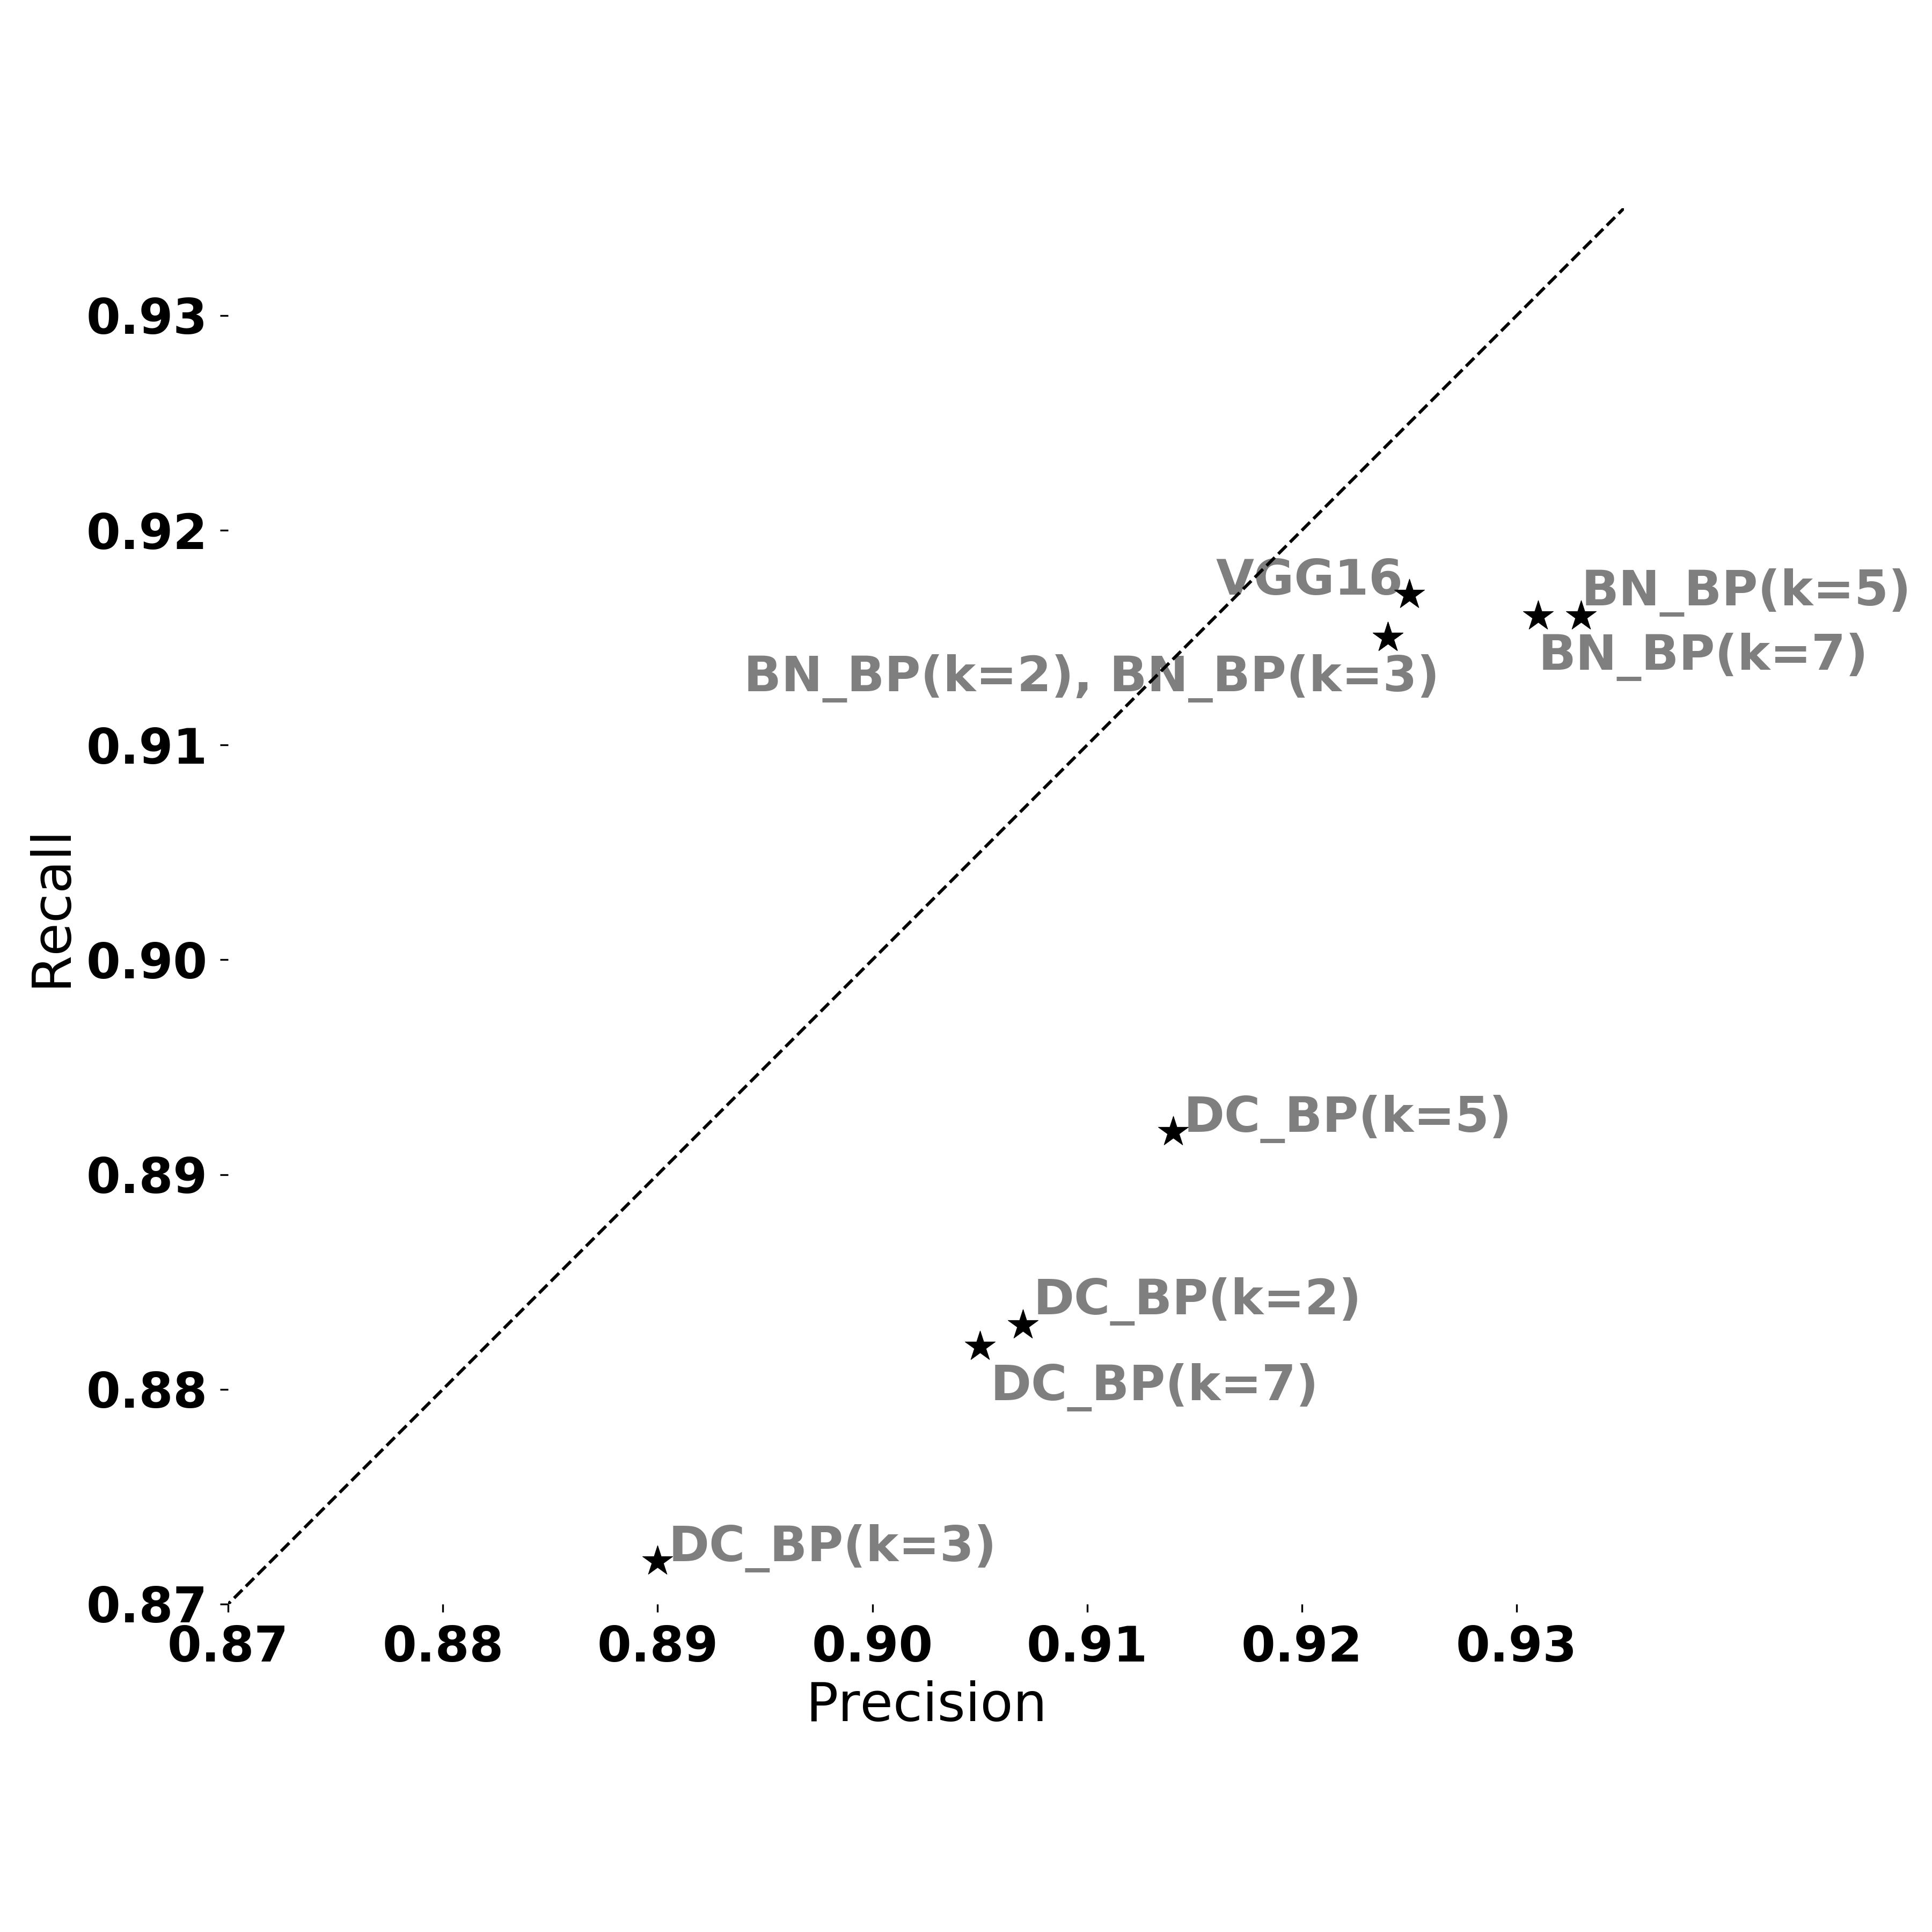
\includegraphics[width=0.85\textwidth]{./thesis_code/plots/precision_recall_curve_all_configs_bw.png}
	\caption{Precision and Recall statistics for each configuration tested. See Table \ref{table:experiment_results} for configurations corresponding to the names in this figure.}
	\label{fig:bestmodel_precision_recall_curves}
\end{figure}

\begin{figure}[h]
	\centering
	\begin{subfigure}[b]{0.45\textwidth}
		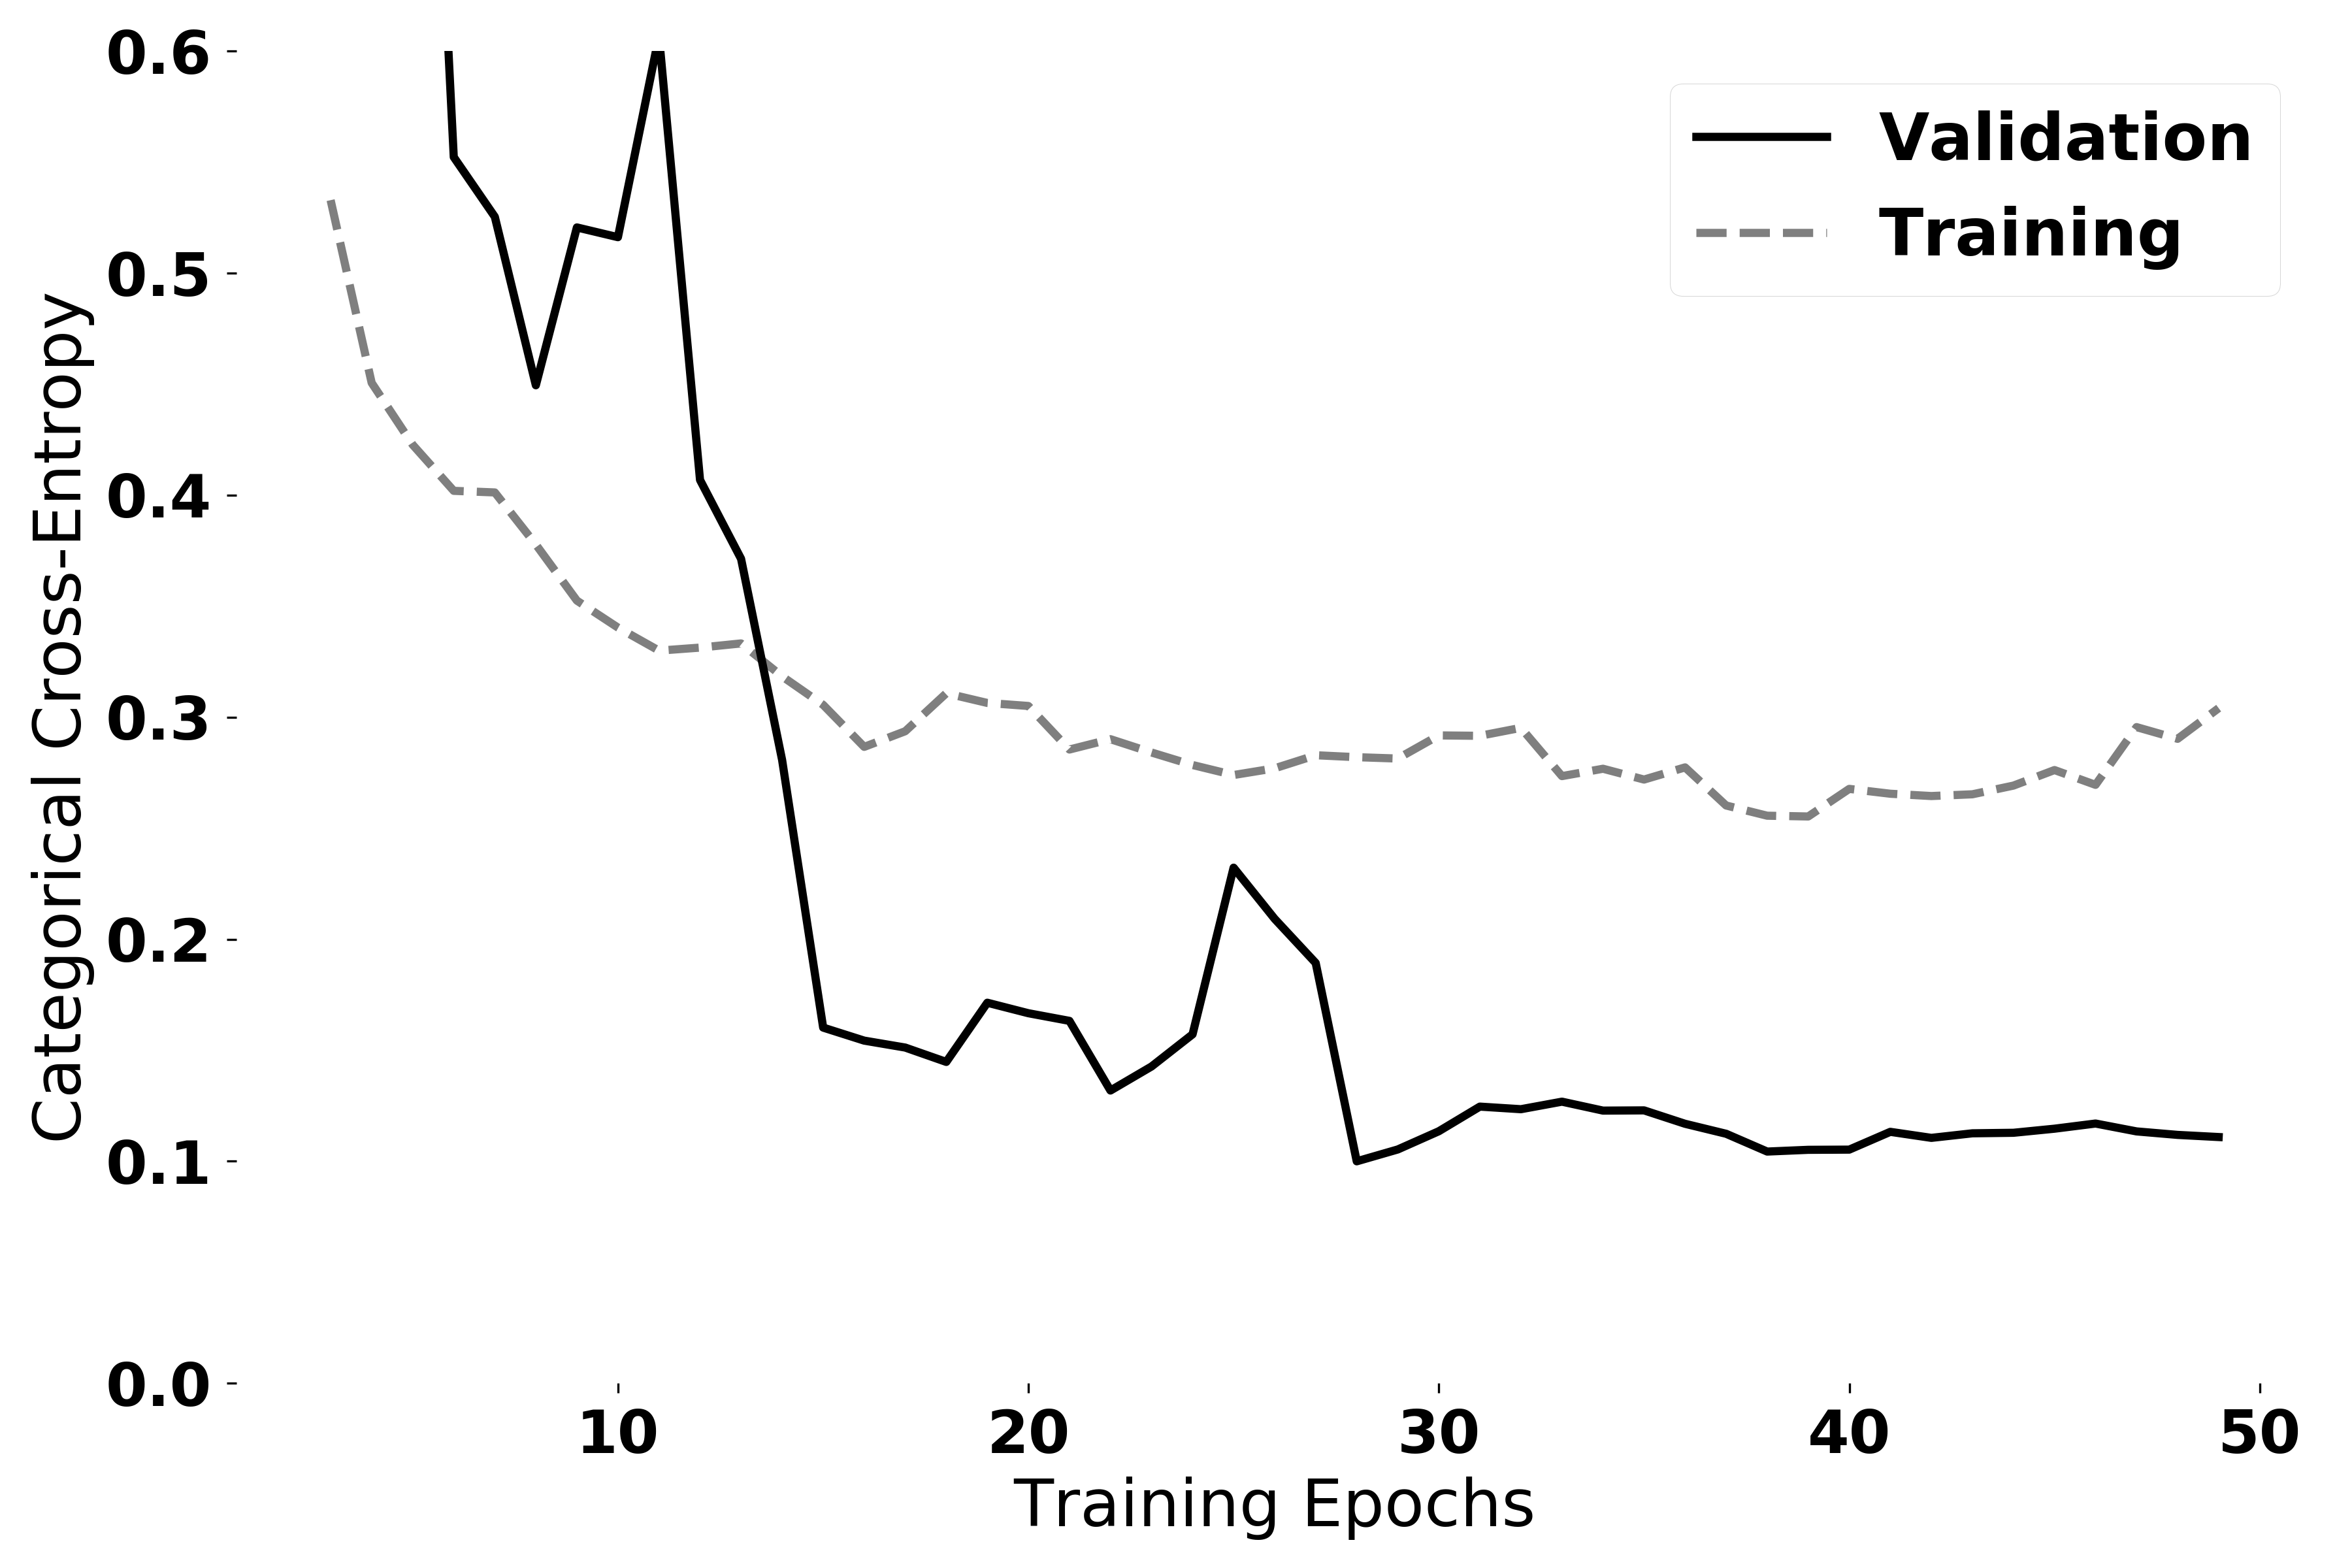
\includegraphics[width=\textwidth]{./thesis_code/plots/20191011_BP_k5_BN_loss_bw.png}
		\caption{Loss}
		\label{fig:bestmodel_first_case}
	\end{subfigure}
	\begin{subfigure}[b]{0.45\textwidth}
		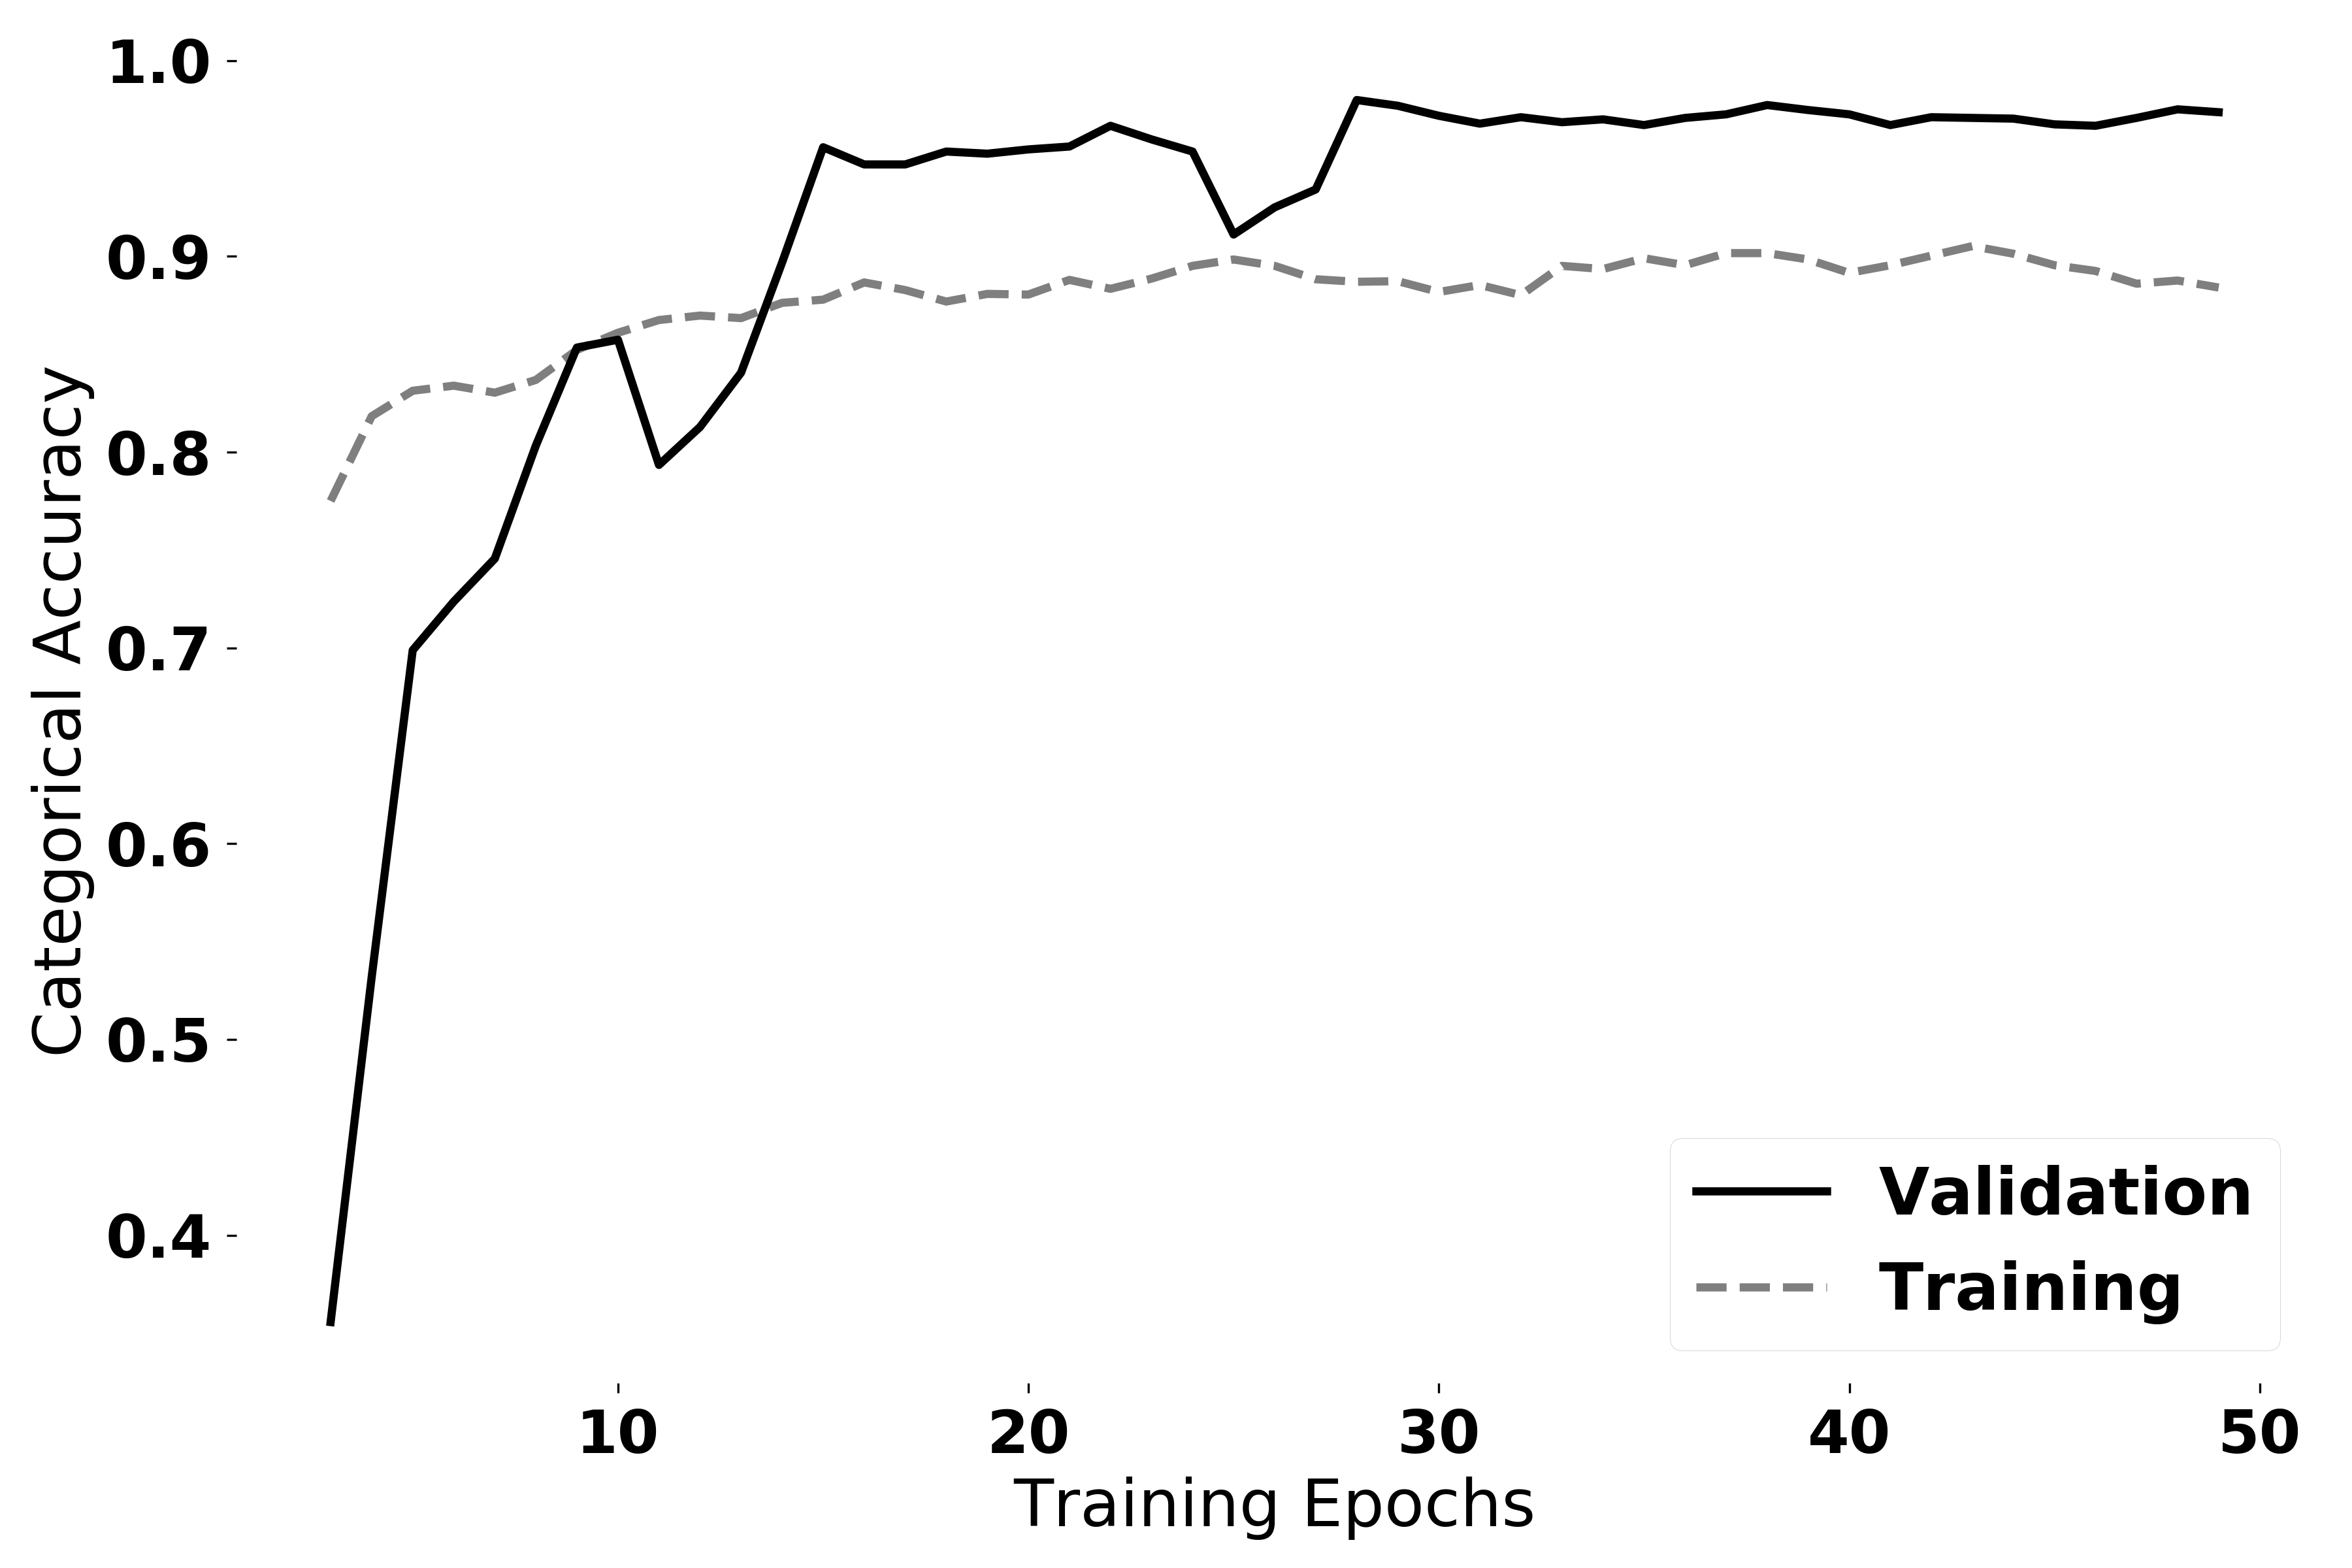
\includegraphics[width=\textwidth]{./thesis_code/plots/20191011_BP_k5_BN_acc_bw.png}
		\caption{Accuracy}
		\label{fig:bestmodel_second_case}
	\end{subfigure}
	\caption{Loss and accuracy curves for our best-case network, which utilized the VGG16 base model feature extractor, with batch normalization layers following each convolutional layer, and BlurPool layers with a kernel size of 5. Training was allowed to progress with base model weights frozen until a loss plateau was reached, before fine-tuning by allowing all parameters to update during training. Fine Tuning began at Epoch 36.}
	\label{fig:bestmodel_fig_sim}
\end{figure}

The results of the described experiments can be seen in Table \ref{table:experiment_results}.
Interestingly, the default configuration given by VGG16 yields very good results, and indeed, has the highest Recall value of any configuration tested.
However, the best overall architecture was that which utilized both batch normalization and BlurPool (k=5).
It registered the highest categorical accuracy as well as the highest precision, and its recall was nearly equivalent to the best-in-class default VGG16.

\section{Classifications on Unseen Data}
\label{sec:bestmodel_newdata}

\begin{figure}[!t]
	\centering
	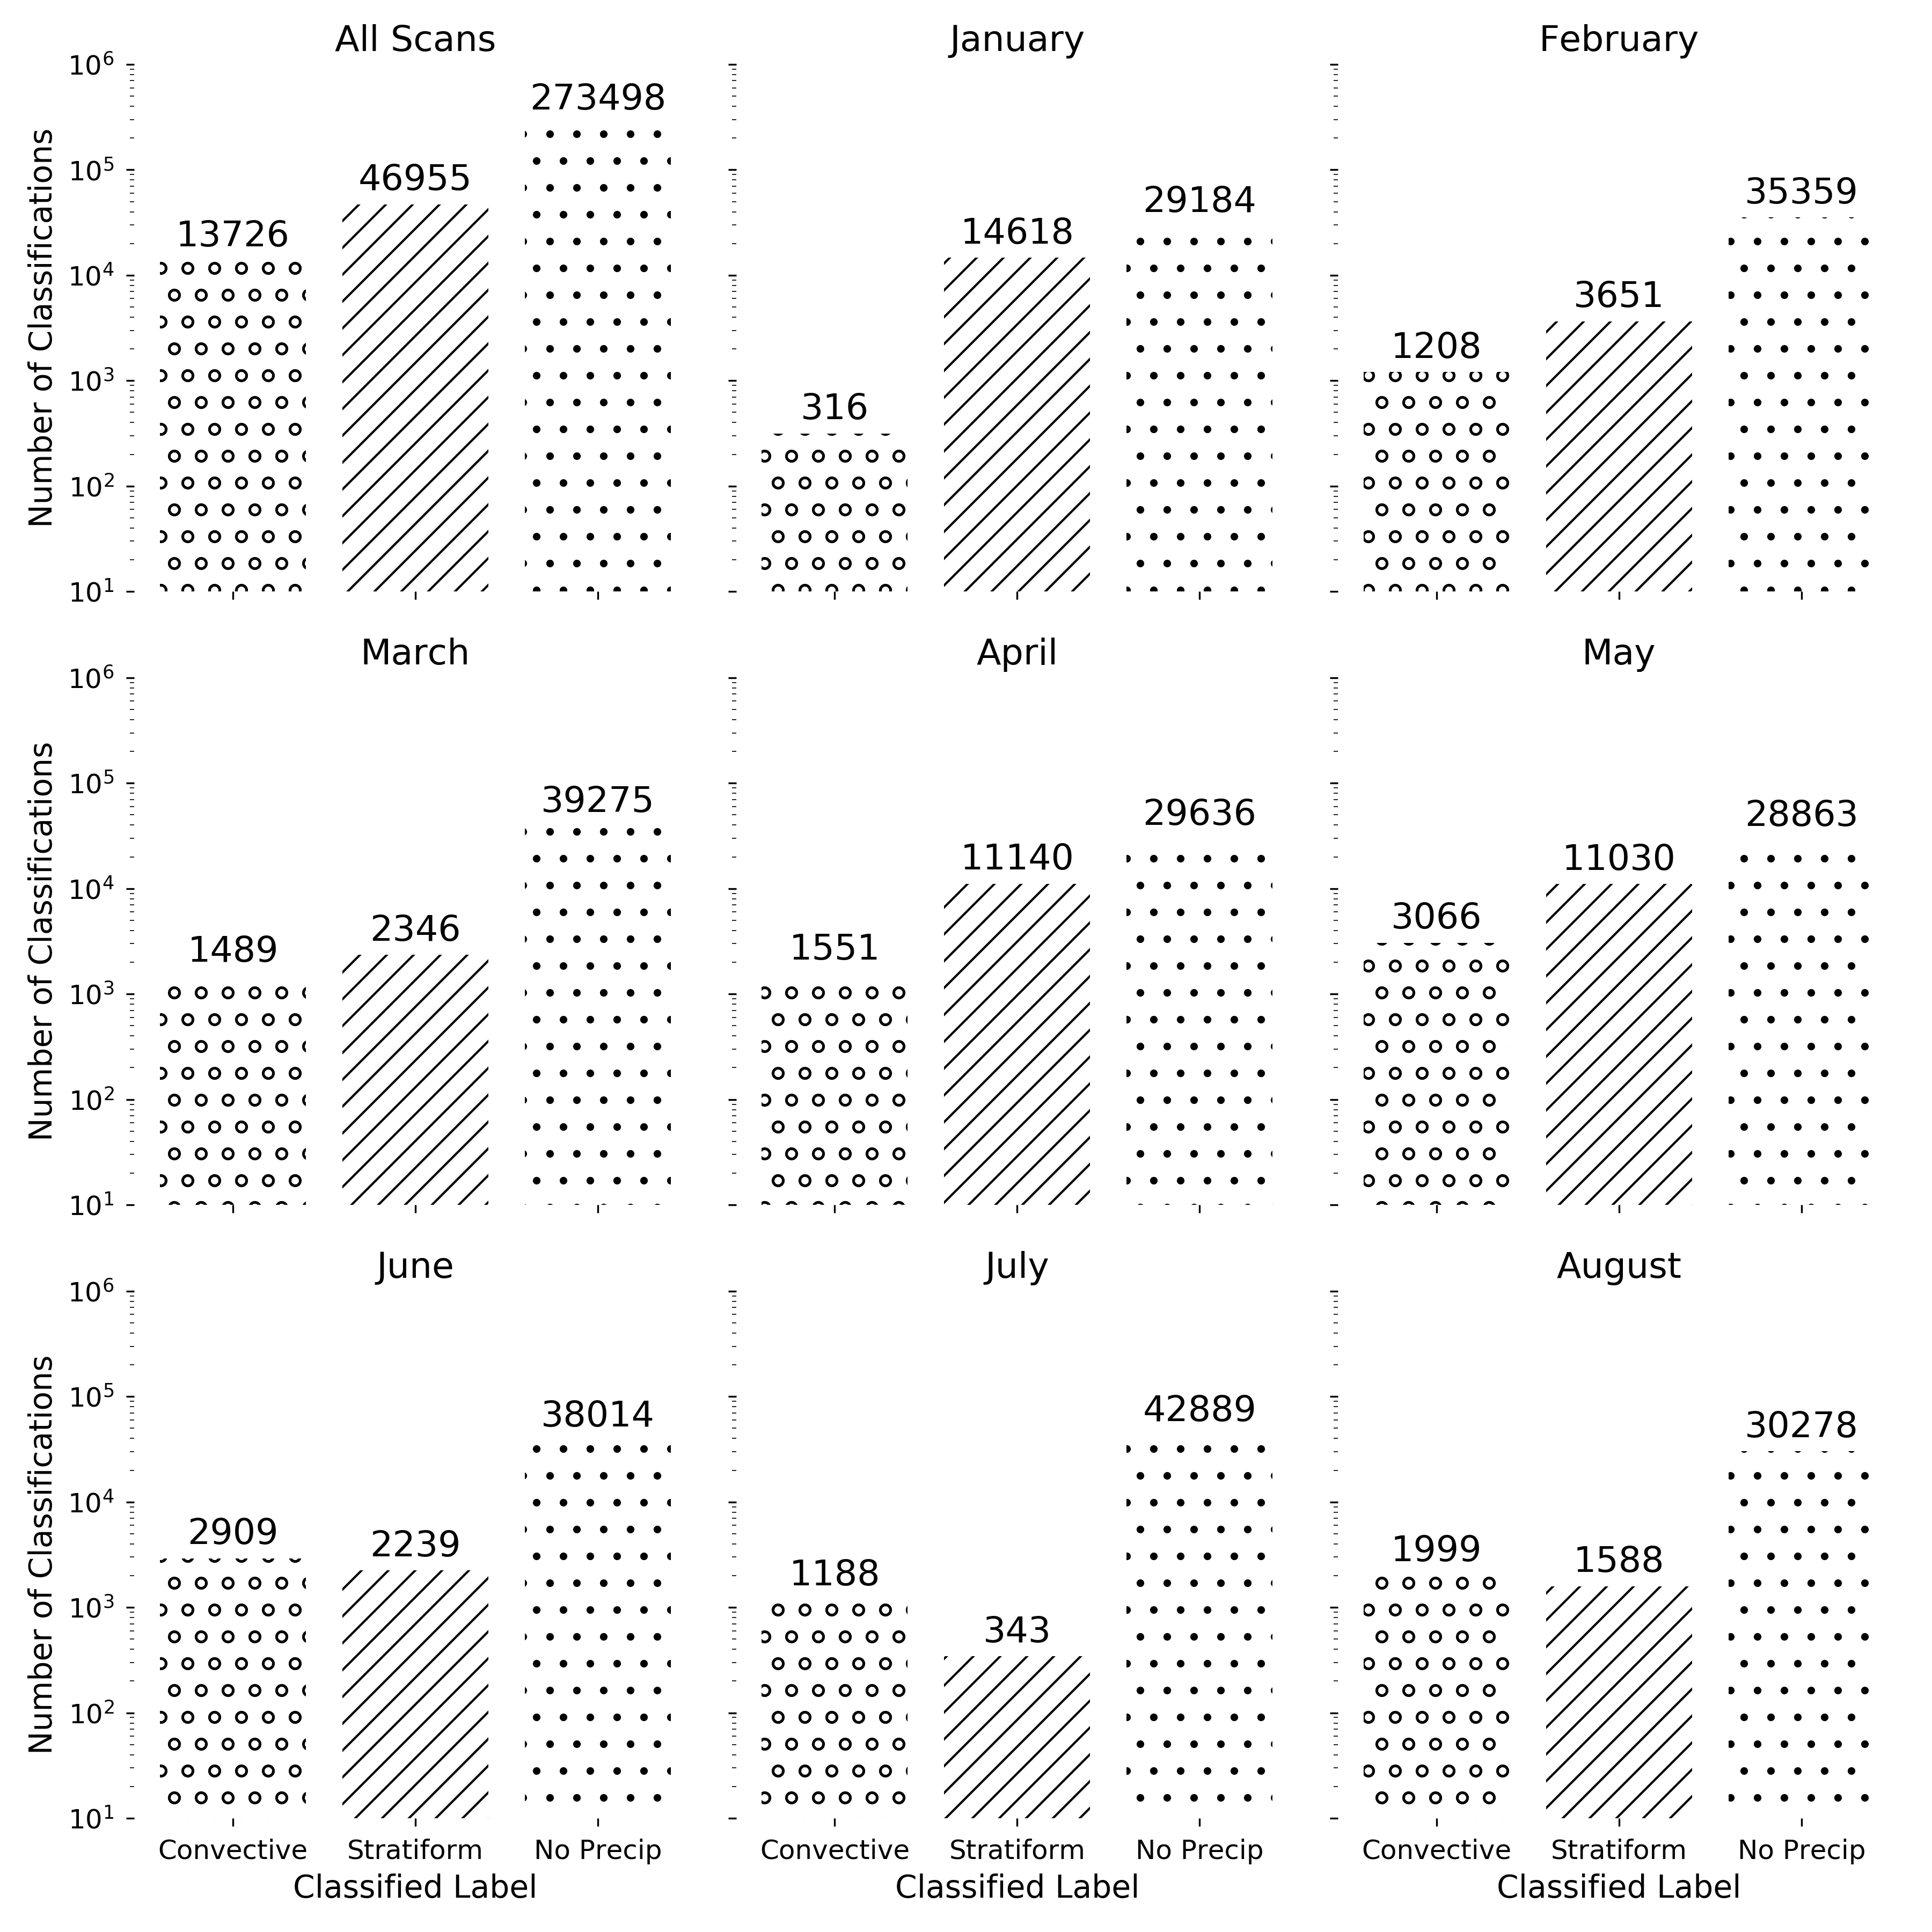
\includegraphics[width=\textwidth]{./thesis_code/plots/2019_predictions_hist_bw.png}
	\caption{The fully trained model was deployed on all scans available from 2019 observed and recorded by the CASA XMDL radar. This set of plots shows the statistics on how images were classified for all months together (top left), and each month individually.}
	\label{fig:bestmodel_all_hists}
\end{figure}

\section{Summary}
\label{sec:bestmodel_summary}

As seen above, the added data has led to a greater level of generalization ability for the deep neural network architecture.
The addition of BlurPool appears to help not only the consistency and generalizability of the model, but also the classification accuracy.
Batch Normalization ensures the training parameters are well-behaved and thus converge to a better minimum in the loss function.
And the newly trained model quickly and efficiently produces believable classifications on large amounts of data in a short period of time.



\chapter{Real-Time Weather Radar with CHORDS}
\label{sec:realtime}
% This whole section is super weak on math, but maybe that is OK
% It just doesn't translate well to papers and dissertations, for one thing
% But also, shows how little support there is for weather radar data
% if our one programmer is unwilling to add it, we are up a creek
% Still, as a survey, perhaps this discussion is important
The issues and solutions presented in this dissertation thus far can be applied to enhance the process of data discovery even further when introduced to workflows involving recent developments in cyberinfrastructure for data. 
To this point, the focus has been on developing methods for identifying interesting and relevant features in historical datasets. 
It is also important, however, to consider real-time data, and the implications of incorporating the aforementioned methods in real-time.

Perhaps some of the most important applications of weather data is in discovering what is happening in the moment, and in predicting what will be happening in the near future. 
The stated goals of many radar networks, including the CASA network and the WSR-88D NEXRAD system, are to provide up-to-the-minute understanding of the ever evolving meteorological systems, to provide disaster warning, transportation planning, and logistical support for people operating within those network coverage regions. 
The data is used as inputs to models to attempt to discern the near-future effects that weather might have at many geographic scales. 
There is an industrial arms-race among start-up and large companies alike to provide hyper-local data of increasing fidelity to capitalize on the financial benefits of providing weather information with lower error rates than competitors, with the added benefit ofdeveloping solutions to augment safety for the populace. 
And there is growing momentum among science communities to develop modern infrastructure to facilitate these goals, within the broader scope of improving the open source, research state-of-the-art.

It is with this last goal in mind that the National Science Foundation (NSF) created EarthCube. 
The EarthCube program has focused on developing an ecosystem where researchers and engineers could focus on the technical and social aspects of modernizing cyberinfrastucture in the geosciences, in tandem with NSF.
The Cloud-HOsted Real-time Data Services for the geosciences (CHORDS) project is the funded project under the EarthCube umbrella that is focused on developing solutions for cost-effective cloud-stored real-time data streaming \cite{kerkez2016cloud}.

This chapter is designed to explain the operating characteristics and functions of CHORDS, as well as the survey of research in integrating weather radar data with CHORDS as informing development of the project.
While Chapter \ref{sec:classifying} illustrates the value designing and deploying models in historical Data Discovery applications, there is also potential for application to real-time streams to provide semantic insights regarding pressing weather concerns, along with populating label databases as data is produced.
It is with this in mind that we survey the current state of the CHORDS project, and discuss its applications to the problem of weather radar data storage, visualization, analysis, and classification, as a way to inform continued development in this active project.

\section{CHORDS}
\label{sec:realtime_chords}
CHORDS in its current format functions as a conduit for managing time series data streams.
The system has been described in \cite{kerkez2016cloud}, but some summary is presented here.
The project developed as the result of an EarthCube workshop, where a group of scientists representing multiple disciplines and multiple universities determined the need for a cross-discipline, remotely accessible platform for handling real-time data streams.
Over the past 6 years, the CHORDS project has evolved and managed a number of use cases, including seismological\cite{jones2017implementing}, hydrological\cite{wong2016real}, and meteorological.
It is this lattermost application that is the focus of this analysis.

A CHORDS Portal is a web application, managed via Docker\footnote{\url{https://www.docker.com/}} containers, and consists of several endpoints.
A researcher manages their real-time stream by first specifying a Site, which is the geospatial location where instruments are placed. 
The instruments themselves are managed on the Instruments page, where a user can specify the properties observed (Variables), and encode information about the observed properties from relevant standards, like SensorML \cite{van2009using}.
The observations themselves, the Measurements, can be visualized via a time series plot illustrating recent data, or can be downloaded via the Data downloads page.
There is also a programmatic API available for REST commands to add data or download, allowing connection to headless servers.
As such, it is straightforward to stream data to plug-ins like Grafana\footnote{\url{https://grafana.com/}} to perform more advanced thresholding and compute relevant real-time statistics.

\section{Specific Gates with Radar and Ground Sensors}
\label{sec:realtime_specificgates}

While the limitations of the CHORDS database with respect to access and number of writes is unable to handle the high bandwidth radar data in an exhaustive, one-pixel-per-Instrument manner, there remains interest in specifying certain radar gate values in this manner.

A weather scan can be thought of as an image, and indeed, this is an appropriate and extremely valuable paradigm. 
However, each radar range gate can also be interpreted as a time series, for each radar variable, and as such can be used as its own CHORDS Instrument.
In this paradigm, each radar variable at a point of interest maps to a CHORDS Variable, and the CHORDS Site can be located in the center of the geospatial area of interest.
In order to managed the fact that each Instrument is in different actual locations, we can pass the latitude and longitude of the radar range gates as Variables themselves, where each measurement is constant.
This is a powerful concept, and has been presented by the author in \cite{gooch2017integration}.
A graphical outline of the CHORDS portal in this setup can be seen in Figure \ref{fig:realtime_chordsportal_specificgates_concept}.

\begin{figure}[h]
	\centering
	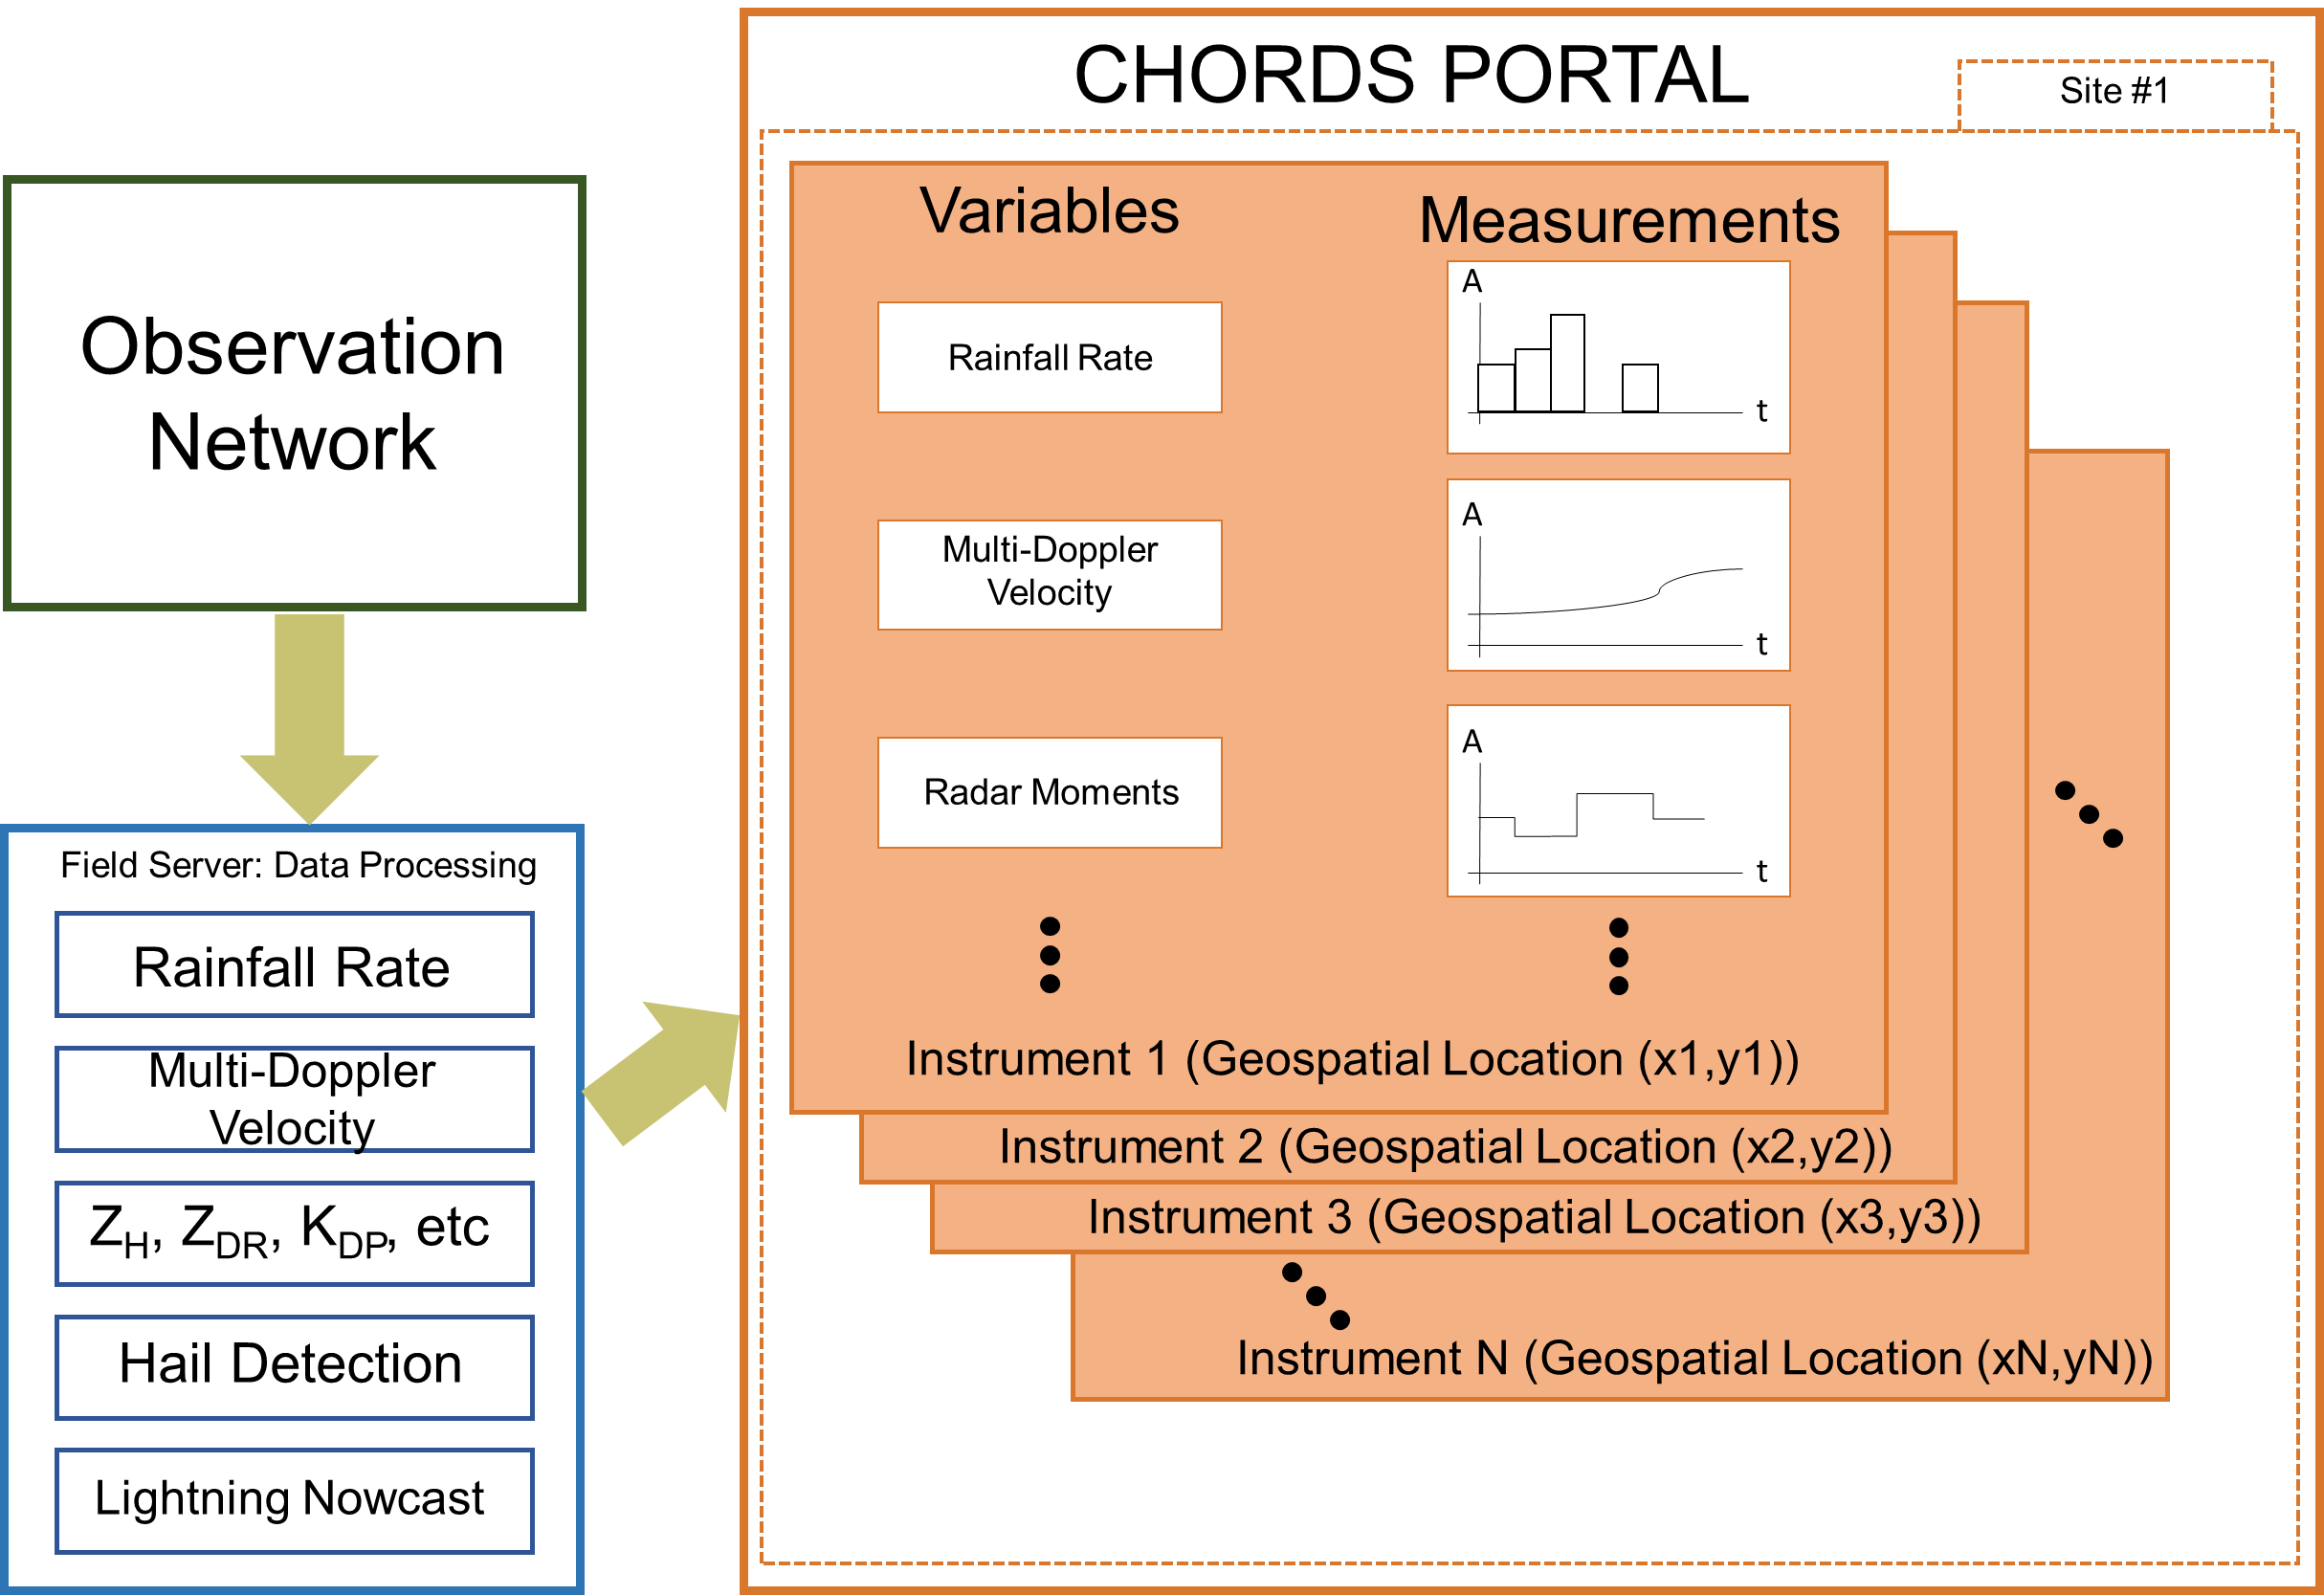
\includegraphics[width=\textwidth]{./thesis_code/plots/chords_portal_concept.png}
	\caption{CHORDS Portal, where selected radar range gates are used as Variables, allowing collocated ground sensors to stream data and provide direct ground-to-radar validation in real-time}
	\label{fig:realtime_chordsportal_specificgates_concept}
\end{figure}

The major gain here is that ground sensors collocated with these radar range gates can be streamed to the same Instrument, allowing real-time validation of either (or both) results.
This was tested using the hydrometeor classification product from the CASA DFW network and ground hail sensor data provided by Understory\footnote{\url{https://understoryweather.com/}}.
See Figure \ref{fig:realtime_chordsportal_hail} to see the benefit of such a setup.

\begin{figure}
	\centering
	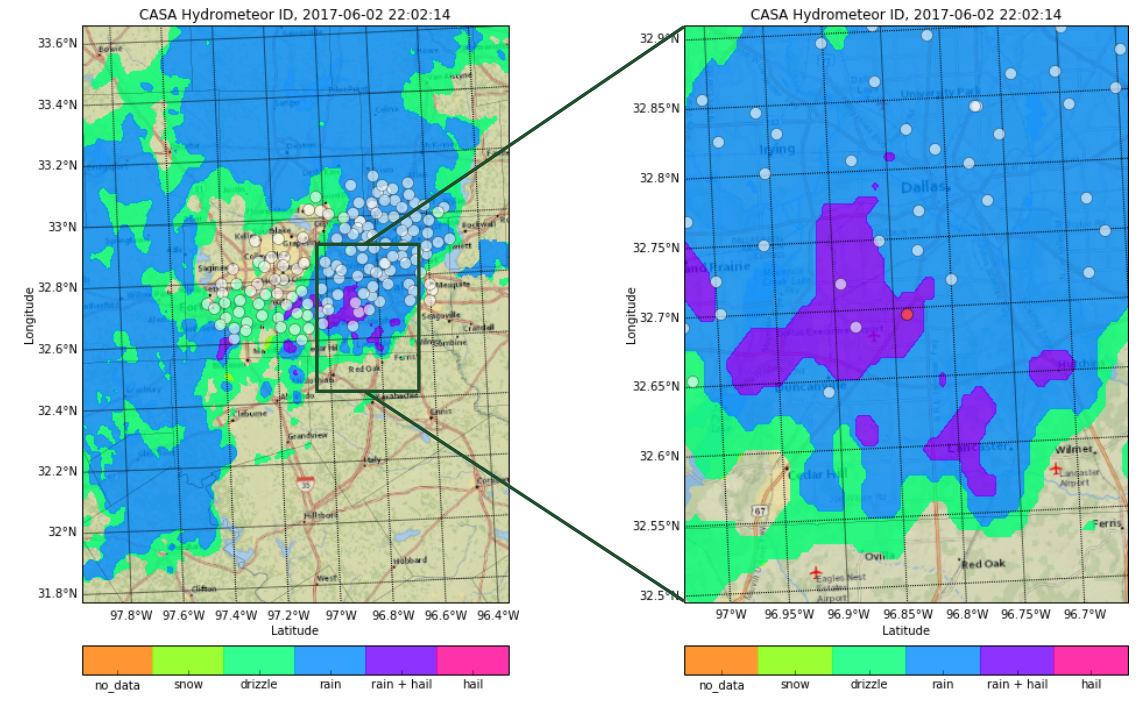
\includegraphics[width=\textwidth]{./thesis_code/plots/hail_radar_hid.png}
	\caption{Aligning hydrometeor identification product with hail sensor hits in the Dallas Fort Worth area, illustrating an example CHORDS use case}
	\label{fig:realtime_chordsportal_hail}
\end{figure}

\section{Full Image Support}
\label{sec:realtime_fullimage}

As of now, full image support has not been implemented, though this research has performed a substantive literature review and various experiments to inform the implementation of full radar image support.
Some of the key concepts and research are presented below.

\subsection{Data Storage}
\label{ssec:realtime_storage}

There are two reasonable methods for storing full radar data in a CHORDS portal.
The first is to simply post full NetCDF files containing completed volume scans.
One benefit to this method is that it opens up a host of potential plug-ins, and allows analysis and visualization of any radar variable.
However, the downside is that this represents an increase in storage footprint, and is a heavier load on server bandwidth.
The main alternative to this is simply passing pre-generated images, such as those presented above.
This is often done at radar operation centers in order to have a human-readable record of historical data, or as a method for generating reports.
As such, it represents lower overhead for the data generation and transmission.
Additionally, as has been shown in this work, there can be useful insight extracted from pre-generated data.
However, this does limit the kinds of analysis that can be performed as plug-ins to the CHORDS portal, and negates the possibility of cross-comparison to collocated instruments, one of the major gains in utilizing CHORDS portals in the preceding section.

\subsection{Data Analysis}
\label{ssec:realtime_analysis}
% Xarray + Dask, talk about how things like Spark and Pandas are great for structured data in tables, but as far as N-D radar data, few strong examples.
% Xarray is nice but unless you have access to tons of RAM, not faster than MATLAB for radar data processing like Zh vs Zdr plots, which would be nice to see in real time, or perhaps rain rate estimators, etc
% So many interesting avenues for real-time analysis, like twiddling sliders and buttons in a jupyter notebook, and populating statistics using most recent scans
% Perhaps too processing intense?

Increasingly, computing and data storage is managed in the cloud.
Various cloud storage and cloud compute platforms have arisen in recent years, leading to cyberinfrastructure developments in the way that data is analyzed.
Given the simplicity of storing data in the cloud, it is reasonable to extend CHORDS-managed data to plug-in to other cloud services.
For the N-dimensional datasets common in geosciences, including weather radar data, there are a few major toolkits worth mentioning:

\begin{itemize}
	\item Xarray\footnote{\url{http://xarray.pydata.org/en/stable/}}
	\begin{itemize}
		\item N-Dimensional array file I/O and analysis package in Python, designed as a NetCDF analysis toolkit. Allows labeled arrays, dataset management, and specification of dimensions, while providing tools for analyzing N-D data borrowed from popular tabular packages (such as pandas\footnote{\url{http://pandas.pydata.org/}})
	\end{itemize}
	\item Dask\footnote{\url{https://dask.org/}}
	\begin{itemize}
		\item Assists packages like Numpy and Xarray by providing straightforward parallelization of common numerical computing functions
	\end{itemize}
	\item Pangeo\footnote{\url{http://pangeo.io/}}
	\begin{itemize}
		\item Closely integrated with the two projects above, Pangeo is a project that seeks to reduce Time to Science for researchers needing to take advantage of cloud compute power, or supercomputers, for large scale analysis.
	\end{itemize}
	\item NetCDF-in-the-cloud
	\begin{itemize}
		\item Another EarthCube project, attempting to provide NetCDF storage to cloud-based data storage platforms
	\end{itemize}
\end{itemize}

\section{Deploying Image Classification in Real-Time}
\label{sec:realtime_classification}

To be added if CHORDS project supports full images in the near future.
\chapter{Summary}
\label{sec:summary}

Data Discovery is an issue of extreme importance throughout the geosciences, where many petabytes of data have been produced, and the speed and quality of the production of the data have outstripped the ability to analyze and tag the data.
Efforts are ongoing throughout the field of geosciences to bridge this gap, enhancing cyberinfrastructure via modern computing and networking capabilities, along with developing the social aspects in managing the need for these developments.
Unfortunately, the effort to extend these advances to the subfield of weather radar data has not present to this point.

The research in this proposal details the current progress in efforts to apply transfer learning techniques to the problem of weather radar image classification, specifically with respect to colormapped images of weather radar data.
A set of experiments was detailed that confirm the capabilities of the chosen end-to-end deep learning model to learn to classify intensity data encoded in images.
Additionally, a hand-labeled dataset of weather radar reflectivity images was generated to aid in training said models, which in turn were used to discover more data.

Once a dataset was labeled and the classifier was trained, the model was deployed on two months worth of unseen data.
These two months were composed of over 85,000 weather radar images and would constitute a laborious, repetitive, and time-consuming task for a researcher if these images were labeled by hand from scratch.
Our first-pass classifier provided classifications on these images that resulted in many true positives, and in a fraction of the time, since each month was fully classified in about one hour on a laptop with GPU.
This first step was a major step forward in terms of historical data discovery of weather radar data as it provided reasonably accurate labels for precipitation regimes in weather radar scans for months' worth of data.

We also extended the effort by hand-curating the predictions on these two months of scans and ensuring false positives were corrected and placed into respective categories.
Utilizing a best-case model determined by theoretical inspection and empirical experimentation, and combining cutting-edge deep learning techniques, we then trained a new model architecture and deployed this on all scans spanning January 2019 through August 2019.
This dataset encompassed over 330,000 weather radar images.
Predicted labels matched climatological expections for the region and time frames, and spot checks of labeled images appear to be generally accurate.

This final effort produced a fully trained deep learning model capable of greater generalization ability, and can be used to identify precipitation regimes in data spanning years at a radar in a single day on constrained compute systems.
It is believed that our research will lead to more expedient data collection periods for researchers, allowing them to perform science more quickly as opposed to being forced to spend greater energy on data collection.
It is also believed that this research has only scraped the surface of what is possible in applying deep learning techniques to weather radar data.
For example, we believe that incorporating other weather radar variables such as specific differential phase and differential reflectivity will yield more accurate classifications, and that extending the model to incorporate these variables extends relatively straightforwardly, if the three-channel pseudo-image approach is used.
Additionally, utilizing more information available in dual-polarization variables may allow image segmentation to occur and lead to a greater number of classifiable categories within the images.
Image segmentation would allow a classifier to identify which pixels in an image correspond to not only stratiform and convective areas, but also may allow discovery of more localized features, such as gust fronts, hail cells, or performing hydrometeor identification.




\backmatter

\bibliographystyle{ieeetr}
\bibliography{gooch_bib} %note that this is a separate file

\appendix %this switches to apppendix mode.  Now any new chapters will be appendices instead of chapters.
\chapter{Appendix A - Tools}
\label{sec:appendix-a-tools}

One of the goals of this dissertation is to provide guidance to both weather radar data specialists and atmospheric scientists in utilizing modern software tools to assist in their research.
 This need, in addition to the cause of providing an in depth look at the entire workflow for the purposes of documentation of academic methods, leads to the formation of this section.

Herein is described the main software and hardware tools that facilitated the research in this document. 
The main programming language and libraries for analysis, machine learning, and display of data will be discussed, in addition to the hardware used in implementing the research stack.

It should be noted that, with the exception of a few tools designed by the author for the express purposes above, these tools are available to all researchers, scientists, engineers, and enthusiasts.

\section{Python}
\label{sec:appendix-a-python}

Python was used for most of the analysis, server design, file handling, and access to machine learning APIs, throughout this work. 
As an interpreted language, it allowed quick prototyping of code and data exploration. 
Its large community of active developers led to the ability to quickly find solutions to issues encountered, while also producing the ecosystem of tools that simplified the process of managing and interpreting data, generating models, and managing reproducible workflows. 
It also directly provided an interface for accessing the data, as well as the hardware tools that made this research possible.

\subsection{NumPy}
\label{ssec:appendix-a-numpy}

Numpy is a python package that exposes an API for creating numerical structures, usually arrays, where the underlying code is written in C.
The functional API is designed following standards, styles, and naming conventions of MATLAB and follows these where possible.

\subsection{Scikit-Learn}
\label{ssec:appendix-a-scikitlearn}

Scikit-Learn is a package under the SciPy umbrella (like NumPy), whose focus is in providing data scientists and machine learning researchers a set of tools to assist common tasks, such as handling datasets and managing pipelines and workflows, along with certain plots.
This toolkit was used in this research mostly with respect to managing the train/val/test splits on the datasets, and in evaluating models.

\subsection{Tensorflow and Keras}
\label{ssec:appendix-a-tf}

Tensorflow, along with its wrapper and API keras, were used to build and train the deep learning networks.
Tensorflow is a large open source package that seeks to harness the power of CUDA-enabled GPUs in training and testing on deep neural networks, while keras is closely tied to Tensorflow and exposes much of its functionality for researchers who may not be experts in computer science.
As its name suggests, the numerical language in Tensorflow are in tensors, where complicated datasets, such as the image datasets in this research, can be succinctly and efficiently represented.
Additionally, while many models are available in so-called \textit{model zoos}, this research used the convolutional bases available in the keras toolkit.
 
\section{Alternatives to Python}
\label{ssec:appendix-a-alternatives}

It is of some importance to mention alternatives to the tools utilized in this research.
Each has its advantages and disadvantages.
The tools used above reflect researcher choice based on previous experience and convenience in implementing the aforementioned tasks, though these could have been implemented in many languages and with many toolkits.

Even within python, there are other packages of note.
Theano can be used directly as an access point for GPU functionality instead of tensorflow.
Another competitor in this arena is Torch, with its python API, PyTorch.
Many researchers also use Caffe, with python wrappers.

Outside of python, R and Julia are potentially useful and in turn used by many data scientists.
And many workflows include components of all of the above, in addition to bash scripting.

Future additions to this proposal include more discussion on the exact workflow used, as well as links to a finalized Github repository for reproducibility. 
\chapter{Computation Hardware}
\label{sec:compute}


\end{document}
